\documentclass[11pt,
  a4paper,
  parskip=half, % This is some extra vertical space between paragraphs, the suggestion is 2cm which is really ugly, so we use what koma script gives us
  % you can also set it to full for even more space. But there is a bad tex style decision: parskip also changes the spacing between listitems such as
  % enumerate and itemize. For this purpose we include the enumitem package and set itemsep=.5em, of course you can change this
  BCOR=10mm, % BCOR is binding correction
  ngerman,
  english
  % if you'd rather have a one sided thesis, add `oneside' to the documentclass
  % oneside,
  % ngerman is needed for hyphenation if the thesis contains parts written in German, switch order with english if you write mainly in English.
  % Remember to change order in the babel package (below) as well.
  % Last language is the preferred one.
  ]{scrbook}
\usepackage[english]{babel} % If you write mainly in English change order to ngerman, english. Also change that in the documentclass options above.
% Include of titling must happen before \title etc.
% that's why it's not in setup.tex
\usepackage{titling}
\title{Development of Galaxy Workflows for Sequence Data Analysis of Notifiable Viral Livestock Diseases}
\author{Viktoria Isabel Schwarz}

\newcommand{\firstexaminer}{Prof.~Dr.~Rolf Backofen}
\newcommand{\secondexaminer}{Prof.~Dr.~Wolfgang Hess}

\newcommand{\advisers}{Dr.~Wolfgang Maier}

% include all packages and define commands in setup.tex

%------------------------------------------------------------------------------
%       package includes
%------------------------------------------------------------------------------
    % font encoding is set up for pdflatex, for other environments see
    % http://tex.stackexchange.com/questions/44694/fontenc-vs-inputenc
    \usepackage[T1]{fontenc}  % 8-bit fonts, improves handling of hyphenations
    \usepackage[utf8x]{inputenc}
    \usepackage{scrhack}
    \usepackage{tikz}
    \usetikzlibrary{fit}

    % ------------------- layout, default -------------------
    % adjust the style of float's captions, separated from text to improve readabilty
    \usepackage[labelfont=bf, labelsep=colon, format=hang, textfont=singlespacing]{caption}
    % With format = hang your caption will look like this:
    % Figure 1: Lorem ipsum dolor sit amet,
    %           consectetuer adipiscing elit.
    %           Ut purus elit, vestibulum
    % If you instead want
    % Figure 1: Lorem ipsum dolor sit amet,
    % consectetuer adipiscing elit. Ut purus
    % elit, vestibulum
    % change to format=plain
    \usepackage{chngcntr}  % continuous numbering of figures/tables over chapters
    \counterwithout{equation}{chapter}
    \counterwithout{figure}{chapter}
    \counterwithout{table}{chapter}

    \setkomafont{chapter}{\normalfont\bfseries\huge}
    \setlength{\parindent}{18pt}

    \usepackage{indentfirst}
    \usepackage{geometry}
    % \usepackage[showframe]{geometry}

    \usepackage{setspace}
    \onehalfspacing

    \usepackage{array}  % custom format per column in table - needed on the title page
    \usepackage{graphicx}
    \usepackage{subfig}  % divide figure, e.g. 1(a), 1(b)...
    \usepackage{amsmath}  % |
    \usepackage{amsthm}   % | math, bmatrix etc
    \usepackage{amsfonts} % |
    \usepackage{calc}  % calculate within LaTeX
    \usepackage[unicode=true,bookmarks=true,bookmarksnumbered=true,
                bookmarksopen=true,bookmarksopenlevel=1,breaklinks=false,
                pdfborder={0 0 0},backref=false,colorlinks=false]{hyperref}
    \usepackage{etoolbox} % if-else commands
    %==========================================
    \usepackage{algorithm,algpseudocode}
    \usepackage{bm}
    \usepackage{tikz}
    \usepackage{svg}
    \usetikzlibrary{positioning}

    % Hurenkind/Schusterjunge
    \clubpenalty=10000
    \widowpenalty=10000
    \displaywidowpenalty=10000

    \usepackage[]{acronym}
    
    % required for the ToDo list
    \usepackage{ifthen}
    
    % for comments and code
    \usepackage{verbatim}

    % Improves general appearance of the text
    \usepackage[protrusion=true,expansion=true,kerning,nopatch=eqnum]{microtype}
    \usepackage{enumitem}

    % nicer font for pdf rendering
    \usepackage{lmodern}
    
    % For nicer looking tables
    \usepackage{booktabs}
    \usepackage{pdflscape}
    \usepackage{longtable}
    \usepackage{makecell} 
    
    % ----------------- referencing ----------------
    \newcommand{\secref}[1]{Section~\ref{#1}}
    \newcommand{\chapref}[1]{Chapter~\ref{#1}}
    \renewcommand{\eqref}[1]{Equation~(\ref{#1})}
    \newcommand{\figref}[1]{Figure~\ref{#1}}
    \newcommand{\tabref}[1]{Table~\ref{#1}}

    \definecolor{darkgreen}{rgb}{0.0, 0.5, 0.0}


    % ------------------- layout -------------------
    \let\mySection\section\renewcommand{\section}{\suppressfloats[t]\mySection}
    \let\mySubSection\subsection\renewcommand{\subsection}{\suppressfloats[t]\mySubSection}


    % ------------------- pdf settings -------------------
    \hypersetup{pdftitle={\thetitle},
                pdfauthor={\theauthor},
                pdfsubject={Master thesis at the Albert Ludwig University of Freiburg},
                pdfkeywords={bioinformatics, galaxy, workflow, genomics, sequence analysis, virus, thesis},
                pdfpagelayout=OneColumn, pdfnewwindow=true, pdfstartview=XYZ, plainpages=false}


    %==========================================
    \renewcommand{\baselinestretch}{1.5} % line spacing
    \definecolor{arrowblue}{RGB}{98,145,224}
    \usetikzlibrary{positioning,arrows.meta}
    \newcommand\ImageNode[3][]{
    \node[#1] (#2) {\includegraphics[width=0.2\textwidth]{#3}};
    }
    \usepackage{dcolumn}
    \newcolumntype{L}{@{\hspace{1.5em}}D{.}{.}{1.1}@{\hspace{1.5em}}}
    \newcolumntype{V}{>{\centering\arraybackslash}m{3em}}
    \newcolumntype{N}{@{}m{0pt}@{}}

    \setlist{itemsep=.5em}  % set distance between items in a list
    
    \newcommand{\ra}[1]{\renewcommand{\arraystretch}{#1}} % increase the space between rows, 1.3 should be fine

	% ToDo counters
	\usepackage{ifthen} % for whiledo-loop
	\newcounter{todos}
	\setcounter{todos}{0}
	% ------------------- marker commands -------------------
    % ToDo command
    \newcommand{\todoit}[0]{\textbf{\textcolor{red}{TODO \\}}\refstepcounter{todos}\label{todo \thetodos}}
    \newcommand{\todo}[1]{\textbf{\textcolor{red}{TODO: #1}}\refstepcounter{todos}\label{todo \thetodos}}
	

\begin{document}
    \pagestyle{empty} % no header and no page number
    % disable hyper links to remove warning "destination with same identifier"
    % this means within this section nothing can be referenced with a hyperlink
    \hypersetup{pageanchor=false}

    % enable/disable, depending on your chosen language
    \begin{titlepage}
\begin{center}

\newcommand{\HorizontalLine}{\rule{\linewidth}{0.3mm}}

{\Large Master Thesis}\\[0.4cm]

% _____________________________________________________________________________
\HorizontalLine \\[0.4cm]
{ \huge \bfseries \thetitle }
\HorizontalLine \\[1.7cm]
% _____________________________________________________________________________

{\Huge \theauthor} \\[2.2cm]

\vfill

\includegraphics*[width=0.36\textwidth]{media/0_0-uni-logo.png}

\Large {
    Albert-Ludwigs-University Freiburg\\
    Faculty of Engineering\\
    Department of Computer Science\\
    Bioinformatics Group\\
    April 28\textsuperscript{th}, 2023\\
}
\end{center}
\end{titlepage}

\thispagestyle{empty}
\ \vfill \ \\ 
\
\textbf{Writing Period}            \smallskip{} \\
October 28th, 2022 -- April 28th, 2023   \bigskip{} \\
\
\textbf{Examiner}                  \smallskip{} \\
\firstexaminer                     \bigskip{} \\
\
\textbf{Second Examiner}       \smallskip{} \\
\secondexaminer                \bigskip{} \\
\
\textbf{Advisor}                  \smallskip{} \\
\advisers

    \pagestyle{plain} % remove chapter name from top, page number at the bottom
    % use \pagestyle{headings} for having the chapter on top of the pages
    % if you wang a more fancy header use \usepackage[automark,headsepline]{scrlayer-scrpage}
    % and read about it in the KOMA script documentation, https://www.ctan.org/pkg/koma-script
    \frontmatter  % roman page numbers
    \chapter*{Declaration}
I hereby declare that I am the sole author and composer of my thesis and that no other sources or learning aids other than those listed have been used. Furthermore, I declare that I have acknowledged the work of others by providing detailed references of said work.  \newline
I hereby also declare that my thesis has not been prepared for another examination
or assignment, either wholly or excerpts thereof.
\\[3\normalbaselineskip]
\begin{tabular}{p{\textwidth/2} l}
  % \textbf{Freiburg, 28.04.2023}         &   \includegraphics*[width=0.4\textwidth]{media/sign.png}\\
  \rule{\textwidth/3}{0.4pt}   &   \rule{\textwidth/3}{0.4pt} \\
  Place, Date                  &   Signature
\end{tabular}

    \chapter*{Acknowledgements}\label{chap:ack}

    \chapter*{Abstract}
\todoit

- What are notifiable viral livestock diseases \\
- main goal: improve surveillance \\
- how? by providing public infrastructure, reference-based mapping, hybrid mapping for AIV/FMDV \\
- why is it the right approach (fast, no knowledge required) \\
- from discussion: summarise findings + evaluate 

    \tableofcontents
    \listoffigures
    \listoftables
    \hypersetup{pageanchor=true}  % re-enable hyperlinking

    \mainmatter  % Arabic page numbers
    \chapter{Introduction}\label{chap:introduction}
Sharing environments means sharing diseases -- this simple relationship expresses how pathogens spread among populations if they get in touch. The affected populations can be animalic or human. Impacts of disease outbreaks can be as severe as the whole world experienced during the pandemic of \ac{COVID-19} that originated in Wuhan, China in 2019. This highly contagious disease was caused by the \ac{SARS-CoV-2}, an infectious virus of presumed zoonotic origin~\cite{wu2020new}. With more than 762.79 million reported cases and more than 6.89 million confirmed deaths as of 13\textsuperscript{th} April 2023, this pandemic is a public health emergency that has caused estimated costs of 16 trillion U.S. dollars. Apart from this, it invoked an outstanding interest in virology research~\cite{covid}. \\
Professionals from many fields, such as public health specialists, researchers, biomedical staff, bioinformaticians and veterinarians are carefully monitoring potentially dangerous viral diseases by examining the viral genome. International managing institutions with a globally distributed network work on safe and healthy environments for both animal and human populations. The \ac{WOAH}, founded as \ac{OIE}, implements standards in animal health and the handling of zoonoses and other diseases. As an intergovernmental organisation following the multidisciplinary One Health principle, it supports its members in the prevention of animal diseases of concern. National veterinary authorities must notify the \ac{WOAH} in case they detect cases of diseases that are listed by the \ac{WOAH}. Modern and high-resolution monitoring of viral diseases include the sequencing of samples with \ac{NGS} platforms and inspecting the viral genome on a base-by-base level. In order to generate the full-length genome sequence in a quality that reliably constitutes the viral genome from the sample, bioinformatic steps are required. Since the motivation for the genomic analysis is given by the large impact and importance in surveillance, these topics are examined below.

\section{Viral Livestock Diseases}\label{sec:viral} 
Infectious diseases caused by viruses that affect domesticated animals, like for example cattle, pigs, goats, sheep, and poultry are referred to as viral livestock diseases. The most frequent and known diseases include Foot-and-Mouth Disease, African swine fever, avian influenza and Newcastle disease. They can spread quickly among animals, and in some cases are transmitted from an animal host to humans, making them zoonotic diseases. There are over 200 known types of zoonoses, some of them, like rabies, being 100\% preventable through vaccination and medication~\cite{who2020zoon}.\\
The term livestock is vague, and generally refers to any breed or animal population that is kept by humans for commercial or useful purpose. According to the 20th Livestock Census of the Department of Animal Husbandry and Dairying, given out by the Indian government, India holds the world's largest amount of livestock with 535.78 million animals as of 2019~\cite{livestock2019}. Not only food production and economy, but also global trade, the agricultural sector and employment rates highly depend on livestock resources. These numbers illustrate the impressive interconnectedness between humans and livestock. The consequences of a collapse of the livestock industry would therefore be significant and far-reaching. 

\subsubsection*{Historic Outbreaks of Zoonotic Diseases}
Historically, zoonoses have shaped serious infectious events. Pathogens that cause zoonotic diseases are viruses (37.7\%), and according to surveillance data also bacteria (41.4\%), parasites (18.3\%), fungi (2.0\%) or prions (0.8\%)~\cite{salyer2017prioritizing}. Prior to the \ac{COVID-19} pandemic modern zoonotic diseases like Ebola virus disease and salmonellosis had high infection rates. Influenza viruses cause epidemics each year, and circulate in all parts of the world. Influenza appears in zoonotic and human-only spreads, but the different types of virus can recombine occasionally and cause events such as the 1918 Spanish flu~\cite{garten2009antigenic, gibbs2001recombination}. Since the first detection of \ac{HPAI} of the H5 subtype in China, 1996 it has been reported in many avian populations worldwide, both domestic and wild. Even though it has adapted to birds as the specific host, the virus can further adapt, spillover to humans and in rare cases be transmitted between humans~\cite{webster1992evolution}. Avian influenza has caused recent seasonal outbreaks, such as the outbreak in 2014 and 2015 in the United States resulting in almost 50 million birds that died as a consequence of an infection or of depopulation~\cite{lee2016highly}. This is roughly a third of the national stock of laying hens. In 2020, there were several outbreaks reported in Europe, almost all with \ac{HPAI} viruses from the H5 subtype~\cite{lewis2021emergence}. It mainly affected farmed ducks due to the high density of animals in the facilities and the separation from wild birds due to domestication~\cite{lewis2021emergence}. The latest outbreak of \ac{HPAI} is spreading worldwide. Having started in early 2022, it has led to more than 58 million culled or died birds. Different H5 subtypes have been reported in 37 countries and so far, six human infections were reported in this outbreak~\cite{authority2023avian}. This number is not nearly as high as for the animals affected, but considering that from 2003 to 2022, there were a total of 868 confirmed cases of H5N1 in humans with a mortality rate of 52\%, each human infection is a risk~\cite{whocumu2023}. The first fatal case of an H3 subtype has been confirmed by the \ac{WHO} just on 11\textsuperscript{th} April 2023, while the infected woman was only the third known case of H3N8~\cite{who2023china}.

\subsubsection*{Risk Factors and Impact of Disease Outbreaks}
Reasons for recurring huge outbreaks of viral diseases in animal confinements are the advantageous circumstances for virus transmission, since it is warm and humid. In general, animal husbandry practises have evolved in the sense that domestic animal species are raised in relatively small and usually confined spaces at a high density. This domestication has given plenty of opportunities to develop more pathogens of viral and bacterial origin over time. The spread of international trading of farm animals has amplified the number of infected animals and the number of infectious diseases. \\
As transmission routes can differ depending on the disease, another factor is transmissibility, determining how easy the infectious agents spread. Vector-borne diseases are transmitted by living organisms that transfer pathogenic microorganisms to other, uninfected animals or humans. Vectors can be mosquitoes, fleas or ticks. Another transmission mode is direct contact airborne transmission. Environmental factors such as a high temperature, humidity and precipitation can facilitate a virus to spread and keep it alive~\cite{eccles2002explanation}. Inadequate food and water supplies, overpopulation and mass migration of animals pose additional risks for transmission of animal diseases in farming surroundings. \\
Outbreaks of livestock diseases do not only affect animal and human health, but also cause high economic losses. Restrictions and containment measures, as well as the culling of animals lead to loss of income for farmers -- since livestock and their products, such as milk, eggs or meat, are used for further production, other businesses that rely on these products are also affected by disease outbreaks.\\
This can reflect in poor growth, production and feed conversion. Another impact of depopulating infected animal populations is the loss of biodiversity within endangered species of wildlife populations~\cite{lacroix2014non, morand2020emerging, reid2010global}.

\subsubsection*{Notifiable Animal Diseases}
For biosecurity and surveillance purposes, the \ac{WOAH} has agreed on a list of notifiable animal diseases that must be reported to in agricultural authorities. This list includes a total of 117 diseases, partly endemic or highly transmissible, such as Foot-and-mouth disease, lumpy skin disease, peste des petits ruminants, classical swine fever, highly pathogenic avian influenza and Newcastle disease~\cite{woah2023list}.\\
Reports of illness cases of animals filed by national veterinary authorities are used to detect unusual incidents, including mortality or sickness of animals and have adverse effects on socio-economic or public health. The notifiable animal diseases include more than 50 wildlife diseases which can impact livestock health~\cite{woah2023list}. As the surveillance of viral animal diseases is still of the highest priority in order to avoid expensive and dangerous outbreaks, this topic is discussed in more detail in the following introductory chapter.

\section{Prevention, Surveillance and Control}
Given the potential danger of disease outbreaks to animal and public health, the question is how to detect, monitor, control and prevent outbreaks in farm animal populations. \\
To avoid the impact that a disease outbreak can have, the best method is to avoid the disease in the first place. This leads to the principle of prevention, which has its main task in reducing the overall risk of a virus spreading. Corresponding measures are vaccinations and hygiene standards. For viral material that reassorts over time as the number of infections increases, the potential for a virus to exploit host cell genes that favour viral growth and survival may be high~\cite{fenner2017maclachlan}. In-depth strategies to prevent viral diseases depend heavily on the characteristics of the virus, taking into account transmission mode, environmental stability, zoonotic risk and pathogenesis. Exclusion of infected livestock and vaccination of potentially infected flocks is increasingly practised worldwide~\cite{fenner2017maclachlan}. \\
Surveillance of viral diseases involves the collection of basic information about the disease, including incidence, prevalence and transmission patterns; the systematic and regular collection and analysis of these data is crucial to obtain a detailed overview of the spread. To gain valuable insights into the origin and characteristics of a viral genome, samples from infected animals are sequenced with modern \ac{NGS} methods to derive information from the reconstructed whole-length viral genome. The need for data has led the \ac{WOAH} to publish the above-mentioned list of notifiable diseases. Based on the data collected, authorities can inform their decisions on the allocation of resources for disease control and other containment activities~\cite{fenner2017maclachlan, who2017one}.
Since efforts in tackling viral disease outbreaks for example by mass vaccination are very expensive, official budgets from the governments are required. This makes it a political responsibility to prevent and control animal diseases. \\
One important component of modern and accurate surveillance systems of viral diseases is the access to relevant data. Technologies to produce \ac{DNA} sequencing data have developed to be very cost and time efficient which makes the study of infectious diseases better and faster. At the same time, the amount of \ac{DNA} sequencing data produced with \ac{NGS}, also known as \ac{HTS} platforms, prove this change. \ac{NGS} platforms include IonTorrent, Illumina and \ac{ONT}. Advances in the biotechnological application and evaluation of these data are revolutionising the field on the molecular level~\cite{suminda2022high}. Sequencing technologies take a key role in describing viral diversity in humans and animals, in detecting pathogens and coinfections, in epidemiologic research about the evolution of viral material and in metagenomic characterisation of new microbial material. This is done by constructing the parts or the complete genetic information of a virus, the genome, where the nucleic acids store this information in single or double strands in a linear or circular sequence. Algorithms and analyses of the viral genome of concern are extensively studied and developed for many purposes. With \ac{NGS} methods, the genome sequence can be precisely determined. More detailed methods that are used for viral animal disease surveillance with \ac{NGS}-based technologies are described in~\chapref{chap:state-art}.

\section{Motivation and Objectives of the Thesis}
Bioinformatics and data analysis are crucial for understanding and monitoring viral diseases. However, there is a lack of knowledge and resources in many parts of the world. This is particularly true for poorer countries with small laboratories and national health organisations that are not well-equipped with modern sequencers and surveillance systems. Additionally, transporting clinical samples across international borders is difficult and expensive. Nonetheless, efforts are made to establish global networks such as the \ac{ZODIAC}. It is an initiative by the \ac{IAEA}, launched in 2021, with five major objectives: (1) Strengthening member states' detection, diagnostic and monitoring capabilities, (2) Developing and making novel technologies available for the detection and monitoring of zoonotic diseases, (3) Making real-time decision-making support tools available for timely interventions, (4) Understanding the impact of zoonotic diseases on human health and (5) Providing access to an agency coordinated response for zoonotic diseases~\cite{zodiac2021}. In collaboration with technical experts from different fields from all over the world, and to support the \ac{VETLAB} Network, the \ac{ZODIAC} project has the resources to provide standardised, easy-access, public and integrated pipelines for virus surveillance on the long-term. This will enable laboratories and veterinarians to monitor and analyse their samples more effectively, leading to early detection and prevention of viral livestock diseases. \\
Due to the outstanding research efforts brought about by the \ac{COVID-19} pandemic, analysis pipelines for \ac{SARS-CoV-2} samples were developed on the Galaxy platform. Galaxy and the implementation of pipelines are discussed in more detail in~\chapref{chap:methods}. Reusing parts of the globally used \ac{SARS-CoV-2} pipeline with \ac{NGS} input data for genomic analysis can help to understand other viruses and ultimately lead to a deeper understanding of viral genomes from isolates. \\
This work is part of the \ac{ZODIAC} project and supports pillar (2) in the development of integrated pipelines that enable laboratories, veterinarians and other health professionals to analyse their data from samples obtained with \ac{HTS} technologies. The developed pipelines concern avian influenza A for subtype identification and genome analysis, a poxvirus pipeline for determining poxvirus genomes sequenced as half-genomes in a tiled-amplicon approach and \ac{FMD} for serotyping and genome analysis.
These viruses are chosen for the availability of test samples that were used for validation of the pipelines, for relevance within the \ac{ZODIAC} project and for their importance concerning animal and public health risk. All three pipelines follow an approach that relies on raw read data and enables monitoring of intra-sample minor allelic variant frequencies. The high resolution allows early warning of epidemiological signs of a changing viruses, specifically important for the assessment of emerging variants in pathogenicity and vaccine sensitivity. The aim is to provide fast, sensitive pipelines that are ready-to-use for surveillance purposes and rely on concepts from \ac{SARS-CoV-2} research. \\
In summary, the lack of bioinformatics resources in many countries poses a major challenge to effective viral livestock disease surveillance. However, established global networks such as \ac{ZODIAC} together with \ac{VETLAB} can provide the necessary resources to enable effective surveillance and analysis of viral animal diseases. This in turn will lead to early detection, insights into transmission routes and changes of the virus, prevention of disease outbreaks and ultimately protect public health and reduce the impact of viral diseases on livestock.

    \chapter{State-of-the-Art}\label{chap:state-art}
In the demand for an effective, high-quality approach to the analysis of isolates from infected animals, molecular studies help to investigate characteristics of the sample. Genome analysis has become an integral part of animal disease surveillance, especially since the advent of high-throughput sequencing technologies in the last 15 years. Next-generation techniques, applications and drawbacks are described below, software tools to use handle \ac{NGS} data, state of the art in poxvirus and avian influenza virus analysis, and lastly pipelines for genomic analysis are discussed.

\section{Next-Generation Sequencing}
\ac{NGS} has revolutionised the field of genomics and virology. With its ability to rapidly and cost-effectively sequence large amounts of \ac{DNA} or \ac{RNA}, \ac{NGS} has enabled researchers to explore genetic and epigenetic variations, identify novel genomic features and investigate the evolution and diversity of viruses. In the following section, applications of \ac{NGS} in genomics and virology are discussed, including the different \ac{NGS} platforms available for sequencing. Finally, pitfalls associated with \ac{NGS}, software and techniques are examined.

\subsection{Sequencing Approaches}
When comparing \ac{DNA} sequencing technologies, there are differences in speed, throughput and volume of sequences. The term ``next-generation'' in \ac{NGS} is used to describe newer technologies in the field and implies a next step in the evolution of sequencing technologies. As sequencing machine technologies evolve rapidly, there are gradations such as ``second-generation'' and ``third-generation''. Following the original Sanger sequencing method from 1977 using radioactivity and gels based on chain termination, second-generation sequencers are advancements of Sanger sequencing that apply sequencing by synthesis~\cite{mardis2008next}. However, equipment is comparably expensive and samples require a high concentration of the \ac{DNA} or \ac{RNA} to be sequenced. In second-generation methods, reactions run in parallel and drastically reduce overall costs compared to Sanger sequencing. They produce short sequence read lengths and are able to detect reads without using electrophoresis. Reads are equal to single fragments of \ac{DNA} or \ac{RNA}. Third-generation sequencing technologies typically generate longer primary reads of \ac{DNA} or \ac{RNA} molecules while maintaining the massive speed and parallelism of the technology~\cite{slatko2018overview}. \\
Not only sequencing methods themselves differ in terms of underlying technologies, but also the overall approach how to handle samples in genomics research can be different. Ampliconic and genomic sequencing represent two alternatives in sequencing that can be applied on the varying \ac{NGS} platforms. Ampliconic sequencing is a targeted sequencing approach that amplifies specific regions of a genome by using \ac{PCR} prior to sequencing. This method is particularly useful for studying very similar sequences in order to detect genetic variations within specific genomic regions. The ARTIC network, a collaborative group of researchers, contributed to the development of ampliconic sequencing for viral genomes, particularly for the detection and analysis of \ac{SARS-CoV-2}~\cite{quick2017multiplex, tyson2020improvements}. The ARTIC protocol uses a specific approach, tiled amplicon sequencing, which involves designing primers that amplify overlapping regions of the target genome. The primers are designed to have a fixed length and to be located at a fixed distance from each other, allowing for complete coverage of the target region~\cite{mamanova2010target}. The amplicons can cover only specific regions of the genome but depending on the primer design also cover the full-length genome. At the same time, genomic sequencing is a \ac{WGS} method that sequences the entire genome without prior amplification. This method allows for a comprehensive analysis of the entire genome, including detection of genomic variations, structural variations, and epigenetic modifications~\cite{quick2017multiplex}.

\subsection{NGS Platforms and Applications}
By far the biggest player in the field of high-throughput sequencing of \ac{DNA} or \ac{RNA} samples is the Illumina platform~\cite{illumina2015introduction}. Illumina sequencing is based on bridge amplification, which creates clusters of copies of each \ac{DNA} fragment. This technique involves repeated synthesis reactions with proprietary modified nucleotides containing a different fluorescent label for each of the four bases A, T, C and G. The reactions are performed over 300 or more rounds, and fluorescence allows for faster detection through direct imaging. All \ac{DNA} and \ac{RNA} is converted to \ac{cDNA} before sequencing, because Illumina sequencing requires it to be attached to a solid surface which is done by attaching adapters to the \ac{cDNA} fragments. An Illumina sequencer outputs data in the form of sequence reads, which are short \ac{DNA} fragments ranging from 50 to 600 base pairs in length depending on the specific instrument and protocol used, e.g. MiSeq sequencer for smaller-scale sequencing applications and HiSeq sequencer for whole-genome sequencing~\cite{illumina2015introduction, slatko2018overview, mardis2008next}. Error rates of Illumina MiSeq and HiSeq sequencers range from 0.1\% to 1\% depending on the experiment and platform used~\cite{illumina2015introduction}. The output data from an Illumina sequencer typically is in the form of raw sequence files in FASTQ format, which contain the base calls and corresponding quality scores for each read. These reads can be used for further analyses.

\ac{ONT} is a third-generation paradigm shifting sequencing technology. It measures changes in ionic current across membranes as single-stranded \ac{DNA} nucleotides pass through a nanopore~\cite{jain2016oxford}. Nanopore-based \ac{DNA} sequencing technologies are purchasable as a portable, small MinION (by \ac{ONT}) device, allowing experts to use it for applications where space requirements or portability are important~\cite{greninger2015rapid, jain2016oxford}. The cyclic mode of sequencing used in second-generation approaches is replaced by sequencing in real-time with user-defined read lengths of up to 10,000 basepairs~\cite{jain2016oxford}. The real-time aspect allows for rapid samples analysis in various settings. Despite its advantages, the main pitfall of \ac{ONT} is its relatively high error rates in single reads of 5\% to 15\% compared to other \ac{HTS} methods~\cite{fu2019comparative, laver2015assessing}. Due to the real-time nature and avoidance of \ac{PCR}, the output quality highly depends on the quality and purity of the input sample. This makes \ac{ONT} alone less suitable for single-nucleotide variant analysis that is required in some diagnostic applications~\cite{bowden2019sequencing, stefan2022comparison}. \\
Other second-generation platforms are Roche/454 pyrosequencing, IonTorrent (Thermo Fisher) technology and SOLiD (Sequencing by Oligonucleotide Ligation and Detection). Third-generation platforms include \ac{SMRT} by Pacific Biosciences (PacBio), nanopore sequencing by \ac{ONT} and MGI sequencing~\cite{rhoads2015pacbio}. 

\begin{figure}[ht!]
	\centering
	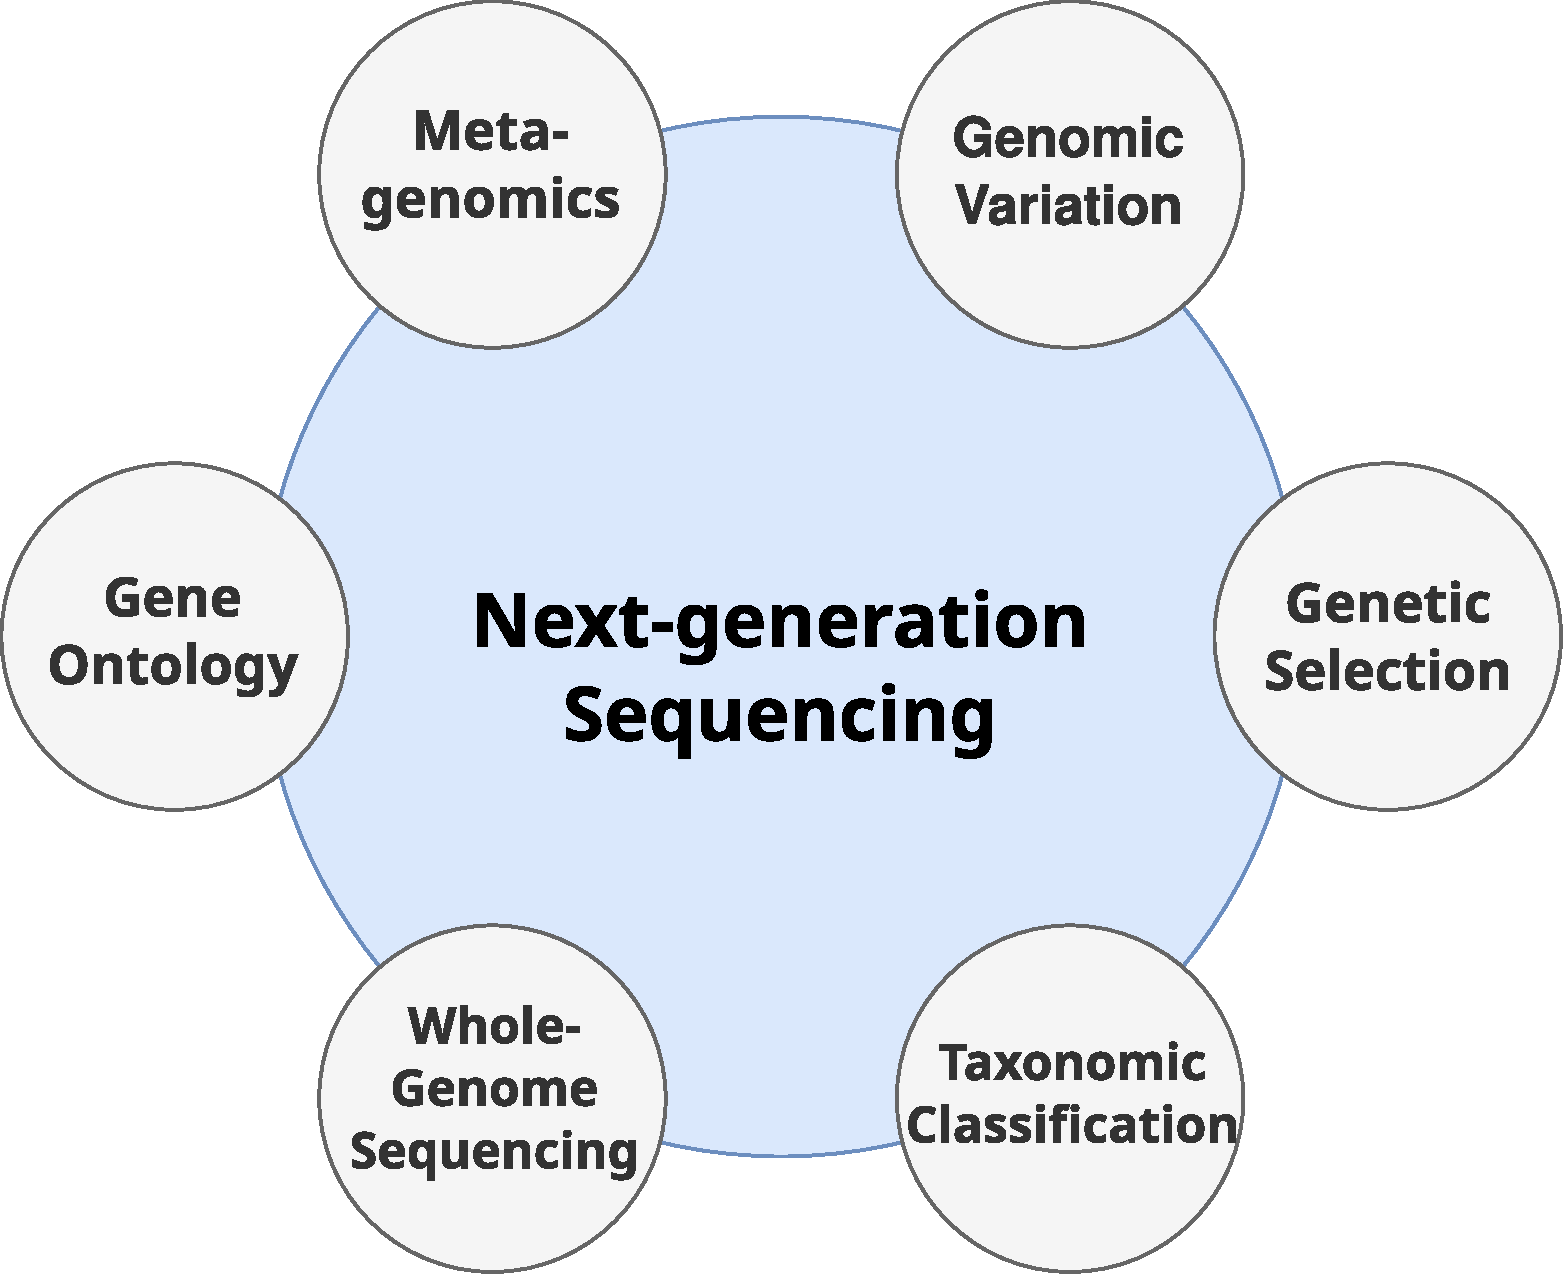
\includegraphics[width=0.65\textwidth]{media/2-ngs.pdf}
	\caption{Applications of next-generation sequencing in different fields.}
	\label{fig:2-ngs}
\end{figure} 

As \ac{NGS} platforms are widely used in biomedical and clinical contexts, some of the most important applications are depicted in~\figref{fig:2-ngs}. Using different tools, hardware and software, samples are prepared for sequencing on an application-specific and available platform and the produced reads can be used for a variety of applications. In virology, metagenomics can be used to identify viruses in complex clinical or environmental samples that contain lots of different nucleic acids~\cite{chiu2019clinical}. It allows for the detection of known and novel viruses without prior knowledge of the infectious agent. Metagenomics involves the sequencing of all genetic material in a sample, including viral genomes, with the aim to identify the presence of viruses and other microorganisms or microbes. This approach is also known as ``shotgun sequencing'' in diagnostics, infection surveillance and the discovery of mutations and pathogens. \\
\ac{NGS} produces huge amounts of data, which can be used to detect genetic variations in samples of clinical patients. Genetic variation refers to finding differences in the form of variations and associating them with particular phenotypes. Genetic variation data of patients are used for personalised treatments or complex disorders. In virology, it refers to differences in the \ac{DNA} sequence of a virus between different strains or isolates. These variants can be used for tracking the spread of an outbreak, identification of sources of an infection, or information about virus virulence~\cite{capobianchi2013next}. Variant detection provides insight to the genome on an every-base level and allows to reliably interpret and identify the many different possible variants~\cite{koboldt2013next}. Specific regions can be sequenced from a sample which is also known as targeted sequencing. \ac{NGS} data can help identify genetic variants that contribute to genomic variations, which can include differences in size, rearrangements, or epigenetic modifications in a nucleic acid sequence. By detecting these genetic variants, \ac{NGS} reads provide insight into the underlying causes of complex diseases or the evolution and virulence of viruses. \\ 
Taxonomic classification describes the placement of samples to existing profiles based on their genetic and structural characteristics. It is a form of clustering analysis and is done by assigning a rank to each read so that a profile is obtained which is used to place it in taxa-specific entities. These entities label and group the sequences. Traditional general-purpose classifiers in microbiology at the genus level are Kraken, Kraken2 and \ac{BLAST}~\cite{wood2014kraken, wood2019improved, altschul1997gapped}.
Taxonomic classification is used for the type identification of a virus causing infections and determination of its potential for transmission or pathogenicity, but also in microbial diversity studies and diagnosis~\cite{dutilh2021perspective}. \\
Another important application of \ac{NGS} is the whole-genome sequencing, allowing a base-by-base view of the sequenced genome. With this approach, large and small variants can be detected. It helps to analyse entire genomes. Since \ac{NGS} methods don't produce the full-length genome at once but generate many reads, the sequencing data are processed and assembled to the complete genome sequence. This can be done by \textit{de novo} assembly without prior knowledge of the genetic origin of the sequenced sample. Assembly software tools generate overlaps of reads and reconstruct the genome without a reference sequence. Alternatively, a reference sequence can be used to map the reads to. \ac{WGS} is used to identify novel viruses, to study mutations in viral genomes and to track the evolution of a virus over time by checking variations on base-level~\cite{slatko2018overview}. It also provides detailed understanding of the genetic makeup of viral pathogens and can help to identify regions that may contribute to pathogenicity or resistance to vaccines. \\
Lastly, gene ontology is applied to \ac{NGS} data in the analysis of genes and their products. It is used to annotate genes and their functions and to compare the gene expression profiles across biological systems. With this approach, it is possible to gain insights to biological processes and molecular mechanisms. With viral samples, it helps to identify pathways that are affected by different disease states, and also to identify biomarkers for diagnosis, treatment and prevention of diseases.

\subsection{Data Analysis Issues}
Since the surveillance of viral animal diseases with \ac{NGS} is advancing rapidly, it is important that health organisations that experience high damage of viral outbreaks but do not have their own facilities and know-how have access to the needed tools and knowledge. Costs for \ac{NGS} sequencers are high and the access to appropriate laboratories is not given everywhere. Networks like \ac{VETLAB} and standardisation of techniques, for example freely available and published by the \ac{WOAH}, can enable professionals worldwide independent of their equipment on site. In the scope of the \ac{ZODIAC} project, this aspect is addressed by providing protocols for each step, starting at sample extraction of potentially infected animals to the detailed analysis and derived actions~\cite{zodiac2021}.

\ac{NGS} methods themselves have downsides that need to be considered when applying these techniques. Generally, chimerical sequences are formed during sequencing, which may be interpreted as false positives for novel organisms if the data are not cleaned. Chimeric products are artefacts originating from joining sequences and are represented by point mutations, insertions and deletions. Chimera formation also occurs during \ac{PCR} amplification~\cite{zylstra1998pcr}.\\
During bioinformatics analysis steps using algorithms with computationally expensive steps, the choice of the algorithm as well as its configuration settings have huge impact on the final results. This includes algorithms in steps such as quality filtering, clustering and sequence classification~\cite{kopylova2016open}. The cleaning step or filtering phase eliminates low-quality reads from the dataset, whereas the error correction process distinguishes true variants from those caused by experimental noise. This is based on the concept that errors occur randomly with low frequency, while true mutations tend to be clustered, and their frequency can be measured~\cite{zagordi2010error}. Longer reads preclude this problem because contigs must not be assembled in the first place, avoiding clustering and filtering errors. This is why the shift in third-generation and later sequencing platforms is towards directly sequencing longer reads. Due to the relatively high error rates of \ac{HTS} technologies that base on the sequencing process itself, \ac{PCR} amplification of the viral material and reverse transcription of viral \ac{RNA} to \ac{cDNA}, it is crucial to include quality checks and filtering steps when using the \ac{HTS} data~\cite{beerenwinkel2012challenges}. \\
Each application of software used with \ac{NGS} data requires expertise in resolving limitations and drawbacks of specific methods. This in turn requires skills and experience in the field and the careful interpretation of results. Nevertheless, \ac{NGS} technologies provide a large pool of methods, although available algorithms for genome assembly and amplicon analysis have drawbacks and limitations~\cite{finotello2012comparative}.

\section{Tools for Genomic Analysis with NGS Data}
A variety of suites and software packages is available to process \ac{NGS}-generated data. Depending on the user's research and analysis interest, tools are used independently and/or subsequently. A tool represents a modular program to use with data input from the user. Different suites for bioinformatic analyses offer different interfaces to execute a tool, either on the command-line to work on a server, or via a web-interface. The software of a tool can be complex algorithms and expensive calculations, or simple and fast formatting programs. \\
Pursuing the goal to construct the full-length genome, short \ac{NGS}-sequenced raw reads in FASTQ format, which is the text-based standard format to store nucleotide sequences with numeric quality scores for each nucleotide, serve as the primary input for any analysis from raw reads. For the central steps of the bioinformatics pipelines described in~\secref{sec:2-general-pipelines},~\ref{sec:2-pox-pipelines},~\ref{sec:2-aiv-pipelines},~\ref{sec:2-fmdv-pipelines} and importantly the proposed pipelines in~\secref{sec:pox-wf},~\ref{sec:aiv-wf} and~\ref{sec:fmdv-wf}, tools and software suites that can work with \ac{NGS}-generated data from different techniques are discussed in the following. 

\subsubsection*{Preprocessing}
Working with raw \ac{NGS} reads requires quality control before executing any further steps. Preprocessing with quality control helps the user to understand the sequencing data and to check its overall quality so that sequencing errors, \ac{PCR} artefacts and contaminations can be detected. Usually, a quality filtering to keep only reads above a certain length and quality threshold is part of preprocessing, as well as when working with ampliconic data, trimming typical sequencing artefacts. The remnants of adapters, artificially introduced during sequencing, need to be removed as they are not part of the transcriptome. Common tools for this purpose are \texttt{FastQC}, \texttt{Trimmomatic}, \texttt{Cutadapt} or \texttt{fastp}~\cite{andrews2010fastqc, bolger2014trimmomatic, martin2011cutadapt, chen2018fastp}. Being developed specifically for adapter-trimming of Illumina and SOLiD data, \texttt{Cutadapt} is a command-line tool written in Python that at the time of publishing was the only tool to support colour-space data. It also provides some read-filtering options~\cite{martin2011cutadapt}. \texttt{Trimmomatic} was developed to solve similar tasks but with higher performance and correct handling of paired-end data. It works with Illumina sequenced data and the user can upload the adapter sequences for adapter trimming if they deviate from standard protocols. It performs quality pruning with a sliding-window cutting algorithm~\cite{bolger2014trimmomatic}. \texttt{FastQC} is a Java-based tool for quality control and provides per-base and per-read quality profiling options~\cite{andrews2010fastqc}. The newest tool for preprocessing, \texttt{fastp}, provides an all-in-one solution for quality control of FASTQ data, which includes all of the options the previously mentioned tools provide. Additionally, \texttt{fastp} outperforms them in terms of speed by being 2 to 5 times faster~\cite{chen2018fastp}. From the point of view of the user who wants to perform all the steps of quality control, filtering and trimming, none of the tools except \texttt{fastp} offers all the functions, which slows down the preprocessing because several tools have to be started. Additional features such as unique molecular identifier preprocessing and per-read polyguanine (polyG) tail trimming are integrated into \texttt{fastp}~\cite{chen2018fastp}. Its multithreading implementation in C/C++ makes it faster than other tools. Reporting of the quality results to compare statistics of the reads before and after the preprocessing run is possible with all tools in combination with \texttt{MultiQC}~\cite{ewels2016multiqc}.

\subsubsection*{Alignment}
In order to obtain the full-length sample sequence and to identify \acp{SNP} in an isolate, short sequenced reads need to be aligned. Assembly of short reads can be done as \textit{de novo} assembly without a reference, however this approach requires great computational capacities and great sequencing depth to ensure a sufficient overlap of the reads for an accurate assembly~\cite{ekblom2014field}. \\
The choice of alignment method depends on the amount, length and origin of read data. In genomic analyses and routine surveillance, this choice can be challenging and typically, fixed references are utilised for mapping the reads against. Often, these are arbitrarily chosen or old sequences. Especially true for RNA virus genome analysis, as with the avian influenza virus, the RNA genome is highly mutable and diverse. This leads to divergence on a regular basis and also leads to antigenic drift. Thus, an intelligent choice of reference sequence for mapping is essential for a meaningful analysis. \\
For reference-based alignment approaches, typically \texttt{minimap2} is used with \ac{ONT}, PacBio or Illumina-sequenced data. \texttt{minimap2} is a pairwise aligner for short reads of at least 100 basepairs in length~\cite{li2018minimap2}. It states to be faster and more accurate than other domain-specific alignment tools~\cite{li2018minimap2}. \\
Other frequently used tools are \texttt{BWA-MEM} for Illumina data and \texttt{Bowtie2} for \ac{ONT} data. Like most other full-genome aligners, \texttt{BWA-MEM} follows the seed-chain-align pattern~\cite{li2013aligning}. Using a Burrows-Wheeler Transform, both \texttt{BWA-MEM} and \texttt{Bowtie2} are shown to be faster aligners than others with reads of 100 basepairs in length~\cite{borozan2013evaluation}. \\
For \textit{de novo} assembly with Illumina, PacBio or IonTorrent data, \texttt{SPAdes} can be used. It is based on a De Bruijn graph algorithm building k-mers~\cite{bankevich2012spades}. For \ac{ONT} or PacBio data to align long error-prone reads, \texttt{Flye} is a modern \textit{de novo} assembler, shown to be highly performant with relatively low error rates~\cite{kolmogorov2019assembly, dida2021empirical}. Its underlying algorithm is an A-Bruijn assembly graph construction that attempts to generate arbitrary paths with overlaps, unlike other De Bruijn-based assemblers which attempt to generate long accurate contigs~\cite{kolmogorov2019assembly}. The A-Bruijn graph is a variant of the De Bruijn graph algorithm that claims to distinguish better between true variants and sequencing errors, and it can more effectively combine repetitive regions into a single assembly sequence~\cite{kolmogorov2019assembly}.

\subsubsection*{Consensus Sequence Construction}
Representing the alignment results in the form of a full-length genome, based on the calculated order of the most frequent residues for each position the consensus sequence is constructed. In a consensus sequence, the most commonly observed nucleotide at each site across the full-length genome is reflected by inference from aligning the sequencing data against a specific reference genome. With aligned Illumina reads, the \texttt{iVar} suite provides tools to generate the consensus sequence. Its features also include primer and quality trimming (\texttt{iVar trim}) and intra-host variant detection (\texttt{iVar variants})~\cite{grubaugh2019amplicon}. On the \texttt{Geneious} platform, similar analyses can be executed in order to produce a consensus sequence from raw reads~\cite{kearse2012geneious}. \texttt{bcftools} as a tool suite also offers a package for consensus sequence construction from \ac{VCF} files~\cite{li2009sequence}.\\
For \ac{ONT} generated data, the \texttt{medaka} tools suite provides a module to generate the consensus sequence from aligned reads. 

\subsubsection*{Phylogenetic Analysis}
Having multiple virus strain samples and wanting to express their relations, evolutionary or phylogenetic trees are a common method to use with nucleotide sequences. Most common tools are \texttt{FastTree}, \texttt{RAxML} (Randomized Axelerated Maximum Likelihood) and \texttt{IQ-Tree}, all based on inferring relations using the maximum-likelihood criterion~\cite{price2009fasttree, stamatakis2014raxml, minh2020iq}. These tools require a multiple sequence alignment as input data, which can be obtained by multiple sequence aligners like \texttt{MAFFT} or \texttt{ClustalW}~\cite{katoh2013mafft, thompson2003multiple}. The generated phylogenetic trees can be visualised to infer topologies and study deep relationships of taxon-groups, while only the \texttt{IQ-Tree} tool provides an in-built visualisation in \textit{.iqtree} format. With the phylogenetic tree in Newick format (\textit{.nhx}) and the \texttt{PhyloCanvas} tree viewer, trees can be exported, extended and visualised with other tools~\cite{abudahab2021phylocanvas}. \\
Other approaches for phylogenetic analysis include a \ac{BLAST} search to identify similar sequences in a database, a widely used method to get an idea of the phylogenetic relationships of the sequence~\cite{altschul1997gapped}.

\subsubsection*{Classification of Sequences}
Many applications of genomic analysis require the placement of the inferred sequence compared to other, similar sequences. Especially in molecular epidemiology, it is useful to query the assembled sequence from the raw reads against a large database of virus genomes. The results give hints for epidemiological linkage or could determine possible regions or countries of origin. This search can be achieved by global alignment or faster techniques based on string comparison. There are many databases available for different categories of sequences, offering database searches to find the closest sequence compared to the query sequence. \\
\ac{BLAST} is a popular search program, while there are different heuristics and variations depending on the specific database and search string characterisations~\cite{altschul1990basic}. For nucleotide sequences and databases, the \ac{NCBI} provides a web-based \texttt{\ac{BLAST}} search form~\cite{johnson2008ncbi, altschul1997gapped}. The underlying algorithm is based on similarity measure that performs a trade-off between speed and sensitivity~\cite{altschul1997gapped}. \\
Having \ac{BLAST} classifying full-length genomes, short sequencing reads can be used for a database search, too.\\
Specifically developed for and tested with influenza reads, \texttt{VAPOR} is a tool that infers a scoring based on a De Bruijn graph construction. It emits the closest sequences from a database of reference sequences~\cite{southgate2020influenza}. \texttt{VAPOR} directly maps reads to a De Bruijn graph without prior assembly and therefore accelerates the classification search as compared to a \ac{BLAST} search while still achieving similar or better results~\cite{southgate2020influenza}. \texttt{VAPOR} provides options to fine-tune the classification run, depending on read length, database size, k-mer size and other measures. It has the option to output a file with the scoring, generated by a scoring function that favours sequences with a high coverage of the reference and those that cover large proportions of the reference~\cite{southgate2020influenza}. It has been argued previously that mapping short reads directly to a De Bruijn graph is less biased than that of mapping to \textit{de novo} assembled contigs~\cite{limasset2016read}.

\section{Pipelines for Genomic Analysis with Viral NGS Data}\label{sec:2-general-pipelines}
In the following, existing pipelines are presented that can be used with unspecified or unknown virus data. They cover parts of the later mentioned pipelines in Sections~\ref{sec:pox-wf},~\ref{sec:aiv-wf} and~\ref{sec:fmdv-wf} and focus on virus discovery, assembly and consensus sequence generation. \\
ViReflow is a pipeline for viral consensus sequence generation and provides a mapping-based approach to variant calling and many optional downstream analyses such as \textit{de novo} assembly and lineage assignment~\cite{moshiri2022vireflow}. The pipeline is based on the Reflow suite, and all computations run in an \ac{AWS} container in a cloud. Reflow emphasises versioning, testing and workflow sharing and does not provide a user-friendly web interface. Instead, it is accessible via a command-line interface. The user chooses from a tool pool of read trimmers, mappers, variant callers and optional downstream analyses. Defaults are \texttt{iVar} for trimming, \texttt{minimap2} for mapping, \texttt{LoFreq} as a variant caller and consensus sequence calling with \texttt{bcftools}. As a result, it may not be as easy to use as Galaxy and its workflows, including workflow development, as this requires programming in Go language. Similar to other pipelines, ViReflow was originally created for the consensus genome construction of \ac{SARS-CoV-2} samples and has been extended for use with all viral genomes~\cite{moshiri2022vireflow}. \\
Another automated pipeline for viral genome assembly, lineage assignment, mutation and intra-host variant detection is V-Pipe, a computational pipeline assessing genetic diversity and introducing a new alignment method \textit{ngshmmalign} specifically for small and highly diverse viral genomes. It includes local and global haplotype reconstruction and a module for detection of flow cell cross-contamination~\cite{posada2021v}. Although V-Pipe is suitable for all viral genomes, it was tested for the identification of the eight influenza segments and successfully identified them from the test sample. V-Pipe is based on Snakemake as a workflow and dependency manager. \\
Other freely available pipelines for the analysis of viral genomes from \ac{NGS} data with several focuses in genomics are VirFind~\cite{ho2014development} and \ac{IRIDA}~\cite{matthews2018integrated}. These pipelines focus on rapid identification of viral materials and do not provide steps for detailed downstream analyses. Automated pipelines for metagenomic \ac{NGS} data are \ac{drVM} and VirMAP~\cite{lin2017drvm, ajami2018maximal}. However, they do not consider the segmented influenza genome and do not provide output data for custom downstream analyses. To our knowledge, there is no freely available pipeline that uses a mapping-based approach that focuses on the viral segments of the \ac{AIV} genome and uses the closest possible reference for each segment. For the various possible downstream analyses, depending on the specific research question, it is critical for a pipeline to provide data outputs and endpoints that enable user-specific assays. This holds not only for avian influenza virus samples, but also for isolates containing other viral material. Galaxy workflows covering the above points for Illumina-sequenced data have been developed in this thesis and are described in~\chapref{chap:methods}.

\section{Poxvirus Analysis}\label{sec:2-pox}
Among the family of poxviruses, there are some diseases that circulate in livestock and pose a risk so that they are on the list of notifiable animal diseases. Among others, mpox, sheeppox and goat pox are the diseases of concern. In the following, characteristics of poxviruses and current approaches to analyse \ac{NGS} data of poxviruses are described.

\subsection{Poxviruses}
Throughout human history, poxviruses have played a significant role with variola being the most notorious as it is the causative agent of smallpox. Smallpox has been described in Chinese texts dating back to the 4th Century AD, and evidence of pox-like scars found on Egyptian mummies suggests the disease may have existed as far back as the 2nd millennium BC~\cite{fenner1988history}. The discovery of a vaccine for smallpox made it the first disease to be eradicated by human efforts, so variola was the first human virus to be successfully eliminated~\cite{fenner2000adventures}. Modern vaccinology owes its origins to Edward Jenner's discovery in the late 18th century that zoonotic infections with the ``cowpox virus'' provided immunity to smallpox~\cite{fenner1988history}. Furthermore, vaccinia virus, which is now used for smallpox vaccination, was the first animal virus to be observed using electron microscopy and the first to be utilized as a vector for transporting foreign genes into animals. This is why poxviruses are among the best-studied viruses. \\
The family of poxviruses, \textit{Poxviridae}, is a family of double-stranded \ac{DNA} viruses. Its natural hosts are vertebrates and arthropods and there are currently 83 species within 22 genera in this family. The \textit{Poxviridae} family is divided into two subfamilies, \textit{Entemopoxvirinae} (insect-infecting viruses) and \textit{Chordopoxvirinae} (vertebrate-infecting viruses). \\
Historically, poxviruses were classified based on disease symptoms and the animal species that was infected. Humans, cows, sheep, goats, horses and pigs have been studied to determine not only clinical symptoms but with the aim to classify poxviruses. This genus classification has been confirmed by recent comparative genome analysis~\cite{gubser2004poxvirus}. Symptoms of disease caused by a poxvirus infection are skin lesions that can differ in size. Depending on the type of poxvirus, the papules can vary from small and pearly papules in infections of \ac{LSDV} to larger crusts and spread generalised pustules in infections with the variola virus. Other general symptoms include fever, headache and rash.

\begin{table}[H]
	\centering
	\begin{tabular}{lll}
	\toprule
	\textbf{Genus}      & \textbf{Virus Species}                          & \textbf{Natural Hosts}                      \\ \midrule
	Avipoxvirus         & Canarypox virus                                 & Songbirds 									\\ 
						& Fowlpox virus                                   & Chickens, turkeys                           \\ \midrule
	Capripoxvirus       & Sheeppox virus                                  & Sheep                                       \\
	                    & Lumpy skin disease virus                        & Cattle                                      \\ \midrule
	Centapoxvirus       & Yokapox virus\textsuperscript{1}                & Humans, mosquitoes                          \\ \midrule
	Cervidpoxvirus      & Deerpox virus                                   & Deer                                        \\ \midrule
	Crocodylidpoxvirus  & Crocodilepox virus                              & Crocodiles                                  \\ \midrule
	Leporipoxvirus      & Myxoma virus                                    & Rabbits, hares                              \\ \midrule
	Molluscipoxvirus    & Molluscum contagiosum virus\textsuperscript{1}  & Humans, primates, birds, dogs               \\ \midrule
	Orthopoxvirus       & Variola virus (Smallpox)                        & Humans (eradicated)                         \\ 
						& Mpox virus\textsuperscript{1}                   & Humans, primates                            \\ 
						& Cowpox virus\textsuperscript{1}                 & Humans, cats, cows, elephants               \\ 
						& Vaccinia virus\textsuperscript{1}               & Humans, cattle, buffaloes, rabbits          \\ 
						& Camelpox virus                                  & Camels                                      \\ \midrule
	Parapoxvirus        & Pseudocowpox virus\textsuperscript{1}           & Humans, cattle                              \\ 
						& Orf virus\textsuperscript{1}                    & Humans, sheep, goats, etc.                  \\ \midrule
	Suipoxvirus         & Swinepox virus                                  & Pigs                                        \\ \midrule
	Yatapoxvirus        & Yaba monkey tumour virus\textsuperscript{1}     & Humans, rhesus monkeys                      \\ \bottomrule
	\textsuperscript{1} Zoonotic disease &                                &                                             \\
	\end{tabular}
	\caption{Representative viruses from ten Chordopoxvirus genera.}
	\label{tab:2-chordopox}
\end{table}

\tabref{tab:2-chordopox} shows ten representatives of the 18 Chordopoxvirus genera according to the newest \ac{ICTV} Taxonomy Release from 2021, while at least five genera contain zoonotic poxviruses~\cite{tax2021virus}. Orthopoxviruses have the biggest impact on human and animal health, and are remarkable for their broad host spectrum ranging from humans to wild and domestic animals~\cite{fenner2000adventures}.
The Chordopoxvirus subfamily is characterised by its large, linear double-stranded genome. Size varies between 134 to 365 kilobases~\cite{brunetti2003complete, tulman2004genome}. Chordopoxvirus genomes contain 130 to 328 \acp{ORF}, and typically, two identical \acp{ITR} are located at both ends of poxvirus genomes. \\
Vaccination is available for smallpox, and the vaccine is even considered protective against symptoms of all orthopoxvirus infections. It is recommended for laboratory staff that works with mpox, cowpox, vaccinia and variola~\cite{cono2003smallpox}. For animals, there is a smallpox-based vaccine that is used to protect elephants against cowpox~\cite{kurth2008rat}. Sheep and goats are broadly vaccinated with an orf vaccine, which is, similar to smallpox vaccine, a live virus. The effective vaccination against existing poxvirus diseases and further microbiological studies, as well as similarities between poxviruses, motivate the expansion of existing data analysis pipelines that work for a specific poxvirus so that they can also work with other poxviruses.

\subsubsection*{Lumpy Skin Disease Virus}
\ac{LSD} is caused by the lumpy skin disease virus belonging to the \textit{Capripoxvirus} (CaPV) genus within the family of poxviruses, subfamily \textit{Chordopoxvirinae}~\cite{walker2019changes}. The \ac{LSD} virus genome is a double-stranded linear \ac{DNA} molecule of circa 151 kilobasepairs in length. It contains between 147 and 156 open reading frames. Similar to other poxviruses, the \ac{LSDV} genome consists of a central coding region which is bounded by two identical \ac{ITR} regions with a length of circa 2,400 basepairs at both ends of the genome. This is a key characteristic to consider during reconstruction of the genome. With a sequence identity of over 96\% with the other \acs{CaPV} genus members sheeppox and goatpox, the \ac{LSDV} genome is highly similar to the other \acs{CaPV} genomes~\cite{tulman2001genome}. \\
\ac{LSDV} is not known to be transmissible to humans and therefore not a zoonosis. Natural hosts of \ac{LSDV} are cattle and Asian water buffaloes. Although \acs{CaPV} is considered to be host specific, sheeppox and goatpox strains can naturally cross-infect in both host species. There have been no cases of natural infection of sheep or goats with \ac{LSDV} reported~\cite{namazi2021lumpy}. The three \acs{CaPV} viruses are the most serious poxvirus diseases of livestock in terms of economic losses in the case of an outbreak. \\
Cattle infected with the \ac{LSDV} typically show symptoms like fever, reduced feed and water uptake and characteristic skin nodules. The number of lesions varies from a few to many, covering the whole body~\cite{prozesky1982study}. From these symptoms alone, it is impossible to differentiate the diagnosis between sheeppox, goatpox and lumpy skin disease. Even with classical methods like cell culture and electron microscopy the highly similar viruses cannot be distinguished. Nowadays, \ac{PCR} and sequencing are the techniques used to provide the sensitive detection of \acs{CaPV}~\cite{lafar2020capripoxvirus}.

\ac{LSDV} has spread from the African continent and since 2019 reached major cattle producer countries in Asia, mainly India, Republic of China and Bangladesh. Other bigger outbreaks in south-west Europe were reported in 2014 to 2018, although these countries opted for a strict vaccination program and successfully eliminated \ac{LSDV} from these regions~\cite{prevention2017control}. In African and Asian countries, veterinarians struggle to fight endemic \ac{LSDV} outbreaks due to lacking financial support by governments, justified by low mortality and morbidity rates. \\
One strain of \ac{LSDV} that has been extensively studied is the ``Neethling'' strain, first isolated in Kenya in 1958. It constitutes the strain used for the live attenuated vaccine that is widely used, if accessible, for cattle against \ac{LSDV}. Some countries use sheeppox vaccines to protect cattle from \ac{LSDV}, even though it does not provide complete immunity. Nevertheless they are used in regions where all \acs{CaPV} are prevalent~\cite{brenner2009appearance}. \\
In 2017, a novel \ac{LSDV} was discovered in Russia, called the Saratov strain~\cite{sprygin2018analysis}. It seems to have arisen through recombination events between field and vaccine strains, which Gershon and his colleagues had predicted much earlier, in 1989, due to the close similarities between Capripoxviruses~\cite{gershon1989poxvirus}. 

\subsection{Pipelines for Genomic Analysis with Poxvirus NGS Data}\label{sec:2-pox-pipelines}
The need for rapid identification of a virus sample to distinguish between species of poxviruses requires sensitive analysis of \ac{NGS} data. Challenges in alignment against a reference are the identical \acp{ITR} at both ends of Capripoxviruses, which is omitted from many pipelines and not part of the analysis, as well as the high identity of 96\%-97\% between the three Capripoxviruses. In order to reach a sufficiently high coverage in all parts of the genome, the reference and the reads can be split into two parts to map against the identical \ac{ITR} regions. With a tiling approach, there is no ambiguity in where to map a read from the \acp{ITR} to. However, the reads have to be sequenced in two pools, which is not the standard protocol. These challenges make it difficult to differentiate between \ac{LSDV}, goatpox and sheeppox~\cite{tulman2001genome}.

An ampliconic assembly-based approach to distinguish Capripoxviruses is described by Mathijs et al.~\cite{mathijs2022robust}. They develop a sequencing protocol in two pools to separate the \ac{ITR} regions. After preprocessing with \texttt{Trimmomatic} and \texttt{FastQC}, the pools of reads are \textit{de novo} assembled with \texttt{SPAdes} and the resulting contigs of each pool are merged into a single contig. To find the correct merging location, an overlap of one amplicon in the middle is assembled in both pools. The test results with various samples show that this approach reconstructs nearly complete \acs{CaPV} genomes. \\
The presented tiling amplicon approach is not usable as an automated pipeline, but can be implemented using the tool specifications in the article. Other viral genomes have been examined in a similar tiling amplicon approach with Illumina, \ac{ONT} or PacBio sequenced data~\cite{grubaugh2019amplicon, freed2020rapid, gardner2014multiplex, quick2017multiplex}. \\
A pipeline of Zhao et al. was designed to study the whole genome of mpox samples~\cite{zhao2016finishing}. After preprocessing with \texttt{FastQC} and the \textit{de novo} assembly step, a neural network method is used for smart gap filling between the assembled contigs. The method shows that gap filling of a genome is an \textit{all k shortest path} (KSP) problem and can be used in an automated pipeline from \ac{HTS} reads to the whole genome sequence. They conclude that it is a promising method to find the ``correct'' sequence, though it did not find the correct sequence assembly for five cases in a sample sequence of mpox~\cite{zhao2016finishing}. Therefore, this method can be used as a guiding first-shot feature, but should not be used for sensitive analyses. Also, the neural-\acs{KSP} method requires knowledge in how to fine-tune the pipeline parameters. \\
Other methods to detect the species of Capripoxvirus of a given sample is nucleic acid extraction and real-time \ac{PCR}~\cite{armson2017detection}. This approach is based on the presence of specific genes to distinguish between Capripoxviruses, but since it does not work with \ac{NGS} data, it does not allow for more analyses and is not comparable to the previous methods.

\section{Avian Influenza Virus Analysis}\label{sec:AIV}
\ac{NGS}-based sequencing data from \ac{AIV} samples need to be thoroughly processed to gain insights into the subtype and variants within the sequence. In the following, the avian influenza pathogen, the avian influenza virus, is described in detail and modern methods in the form of automated pipelines for the analysis of such data are presented.

\subsection{Avian Influenza Virus}
Informally known as bird flu, avian influenza is a viral infectious disease that affects wild birds and poultry. The \ac{AIV} has occasionally crossed the species barrier and infects mammals, including humans. This makes it a high-priority zoonotic viral disease that has been designated as notifiable by \ac{WHO} and \ac{WOAH}~\cite{woah2023list}. Avian influenza occurs in two variants that determine severity: \ac{LPAI} and \ac{HPAI}, with only \ac{HPAI} cases requiring notification. The virus spreads indirectly via contaminated material, e.g. feed, water supplies, feces or feathers. It is transmitted directly from bird to bird via the air, mainly through the transregional movement of wild birds and through long distance bird migration, and in the poultry industry in closed confinements. Humans become infected through close contact with infected material, and most reported human avian influenza infections are from farm workers and others who are exposed in markets, production or clinical contexts~\cite{webster1992evolution}. \\
Symptoms of severe illness are characterised by influenza-like signs such as fever, nasal discharge, coughing and conjunctivitis. This applies to infections in both humans and mammals, while infected birds show signs such as swollen heads, loss of appetite, breathing difficulties and a decrease in egg production.

\ac{AIV} contains a negative-sense, single-stranded segmented \ac{RNA} genome, and due to the segmented nature of the virus, co-infection of different influenza strains can lead to reassortment events. Avian influenza viruses are members of the \textit{Orthomyxoviridae} family and the four species of influenza viruses A, B, C and D are distinguished on the basis of the presence of the \ac{NP} and matrix (M1) proteins~\cite{webster1992evolution}. \ac{AIV} subtypes are determined by the \ac{HA} and \ac{NA} segments and only occur in the influenza A strain, which include all known influenza A virus subtypes H1-H16 in combination with N1-N11, resulting in subtype designations such as H5N1 or H7N9~\cite{webster1992evolution, krammer2018influenza}. To be infectious, a virus particle must contain one of eleven proteins in each of the eight unique segments PB2 (polymerase), PB1/PB1-F2 (polymerase), PA/PA-X (polymerase), \ac{HA}, \ac{NP}, \ac{NA}, M1/M2 and NS1/NEP (distinct non-structural proteins). Genome size differs due to different possible combinations of proteins, though the typical size of a H5N1 genome is 13.5 kilobases. Mutations in the \ac{HA} and \ac{NA} genes occur relatively frequently due to the prone-error \ac{RNA} polymerase in the viral genome which lacks the proof-reading exonuclease activity. \ac{LPAI} subtypes H5 and H7 usually infect poultry, although the natural hosts of avian influenza A are wild waterfowl. These subtypes can transform into \ac{HPAI} during circulation in poultry stocks by recombination with other gene segments or the host genome~\cite{webster2006h5n1}. Both \ac{LPAI} and \ac{HPAI} infections have been reported in domestic poultry, i.e. ducks and chickens, turkeys, caged birds, aquatic birds and wild birds. While some influenza species infect specific animal hosts, all of them can infect pigs and humans. \\
Influenza A strains are the most virulent virus species, and have caused all major historic flu outbreaks through reassortment. Subtypes H5, H7 and H9 are responsible for the largest outbreaks of \ac{AIV} that also spread to humans~\cite{widdowson2017global}. The first confirmed report of human infection with an animal avian influenza virus dates to 1958, and since then 16 subtypes have been detected in humans~\cite{kluska1961demonstration}. Zoonotic spillover events have become increasingly common since the early 20th century and have led to major endemics such as a huge H5 outbreak in the U.S. in 2014/2015. It resulted in more than 25 million bird deaths~\cite{seeger2021poultry}. A current \ac{AIV} outbreak is resulting in more than 58 million dead birds and costs of around 661 million U.S. dollars, which began in 2022 and is spreading across the U.S.~\cite{usda2023hpai}. 
Vaccination against \ac{HPAI} in poultry are used worldwide to ward off avian influenza. They also serve as a preventive measure in the event of an outbreak to reduce the risk of introducing the virus into poultry populations~\cite{swayne2013current, swayne2011assessment}. 

\subsection{Pipelines for Genomic Analysis with Avian Influenza Virus NGS Data}\label{sec:2-aiv-pipelines}
Surveillance systems in the field of genotyping emerging viral strains include classical phylogenetic methods far classifying viral strains, assessing tree topologies, distinguishing between novel and emerging strains, and discovering novel disease-causing variants~\cite{koboldt2013next}. These analyses are essential given the high genetic variability of the genome, and since it consists of eight segments, specific bioinformatics workflows are required for the analysis. \\
The challenge in identifying subtypes and detecting variants lies in the diversity of \ac{HA} and \ac{NA} genes, the main targets of the host immune response. The \ac{HA} and \ac{NA} genes have evolved into several subfamilies and require a dynamic reference selection approach for sequencing analysis. There is a growing number of web platforms, suites and pipelines that enable the analysis of influenza-specific samples with \ac{NGS} data and resources for further analysis, e.g. Influenza Research Database/FluDB~\cite{zhang2017influenza}, EpiFLU/GISAID~\cite{shu2017gisaid}, Nextflu~\cite{neher2015nextflu}, NCBI Influenza Virus Resource~\cite{bao2008influenza}, FluNet~\cite{flahault1998flunet} and OpenFluDB~\cite{liechti2010openfludb}. Many existing suites for automated analysis of influenza samples are based on \ac{SARS-CoV-2} research and have been adapted for the similarly large influenza genome. \ac{INSaFLU} and \ac{PAIVS} are two pipelines specifically designed for the analysis of \ac{NGS}-generated (avian) influenza samples and are discussed in more detail below.

\subsubsection{INSaFLU}
One prominent pipeline for viral metagenomic detection and routine genomic surveillance, \ac{INSaFLU}, provides a web-based protocol for data generated by Illumina, IonTorrent or \ac{ONT} sequencers~\cite{borges2018insaflu}. It is an influenza-focused suite to process \ac{NGS} data to automatically get outputs to answer key questions in influenza genomic surveillance. \ac{INSaFLU} can be used for seasonal influenza, avian influenza, \ac{SARS-CoV-2}, mpox virus or \ac{RSV}. For unspecified viruses, a generic pipeline is provided. The \ac{INSaFLU} pipeline consists of the following steps: (1) Reads quality analysis and improvement with \texttt{FastQC} and \texttt{Trimmomatic}, (2a) classification using a \textit{de novo} assembly with \texttt{SPAdes} and searching a provided database with \texttt{ABRIcate}. Alignment is performed with mapping against a user-input reference sequence and the \texttt{BWA} tool. In the following, (2b) mutation detection and consensus generation with \texttt{Prokka} and \texttt{Snippy} (using the \texttt{Medaka} suite for \ac{ONT} data), (3a) intra-host minor variant detection using \texttt{FreeBayes}, (3b) alignment and phylogeny with \texttt{FastTree} and the tree visualiser \texttt{Phylocanvas}, and lastly (3c) coverage analysis with a \ac{INSaFLU} specific Python script are performed. Using the output data of step (3b), a downstream integrative phylogenetic and geotemporal analysis with Nextstrain can be started. A reference sequence for the mapping step must be provided by the user as input data from the beginning. Currently, \ac{INSaFLU} is accepting \ac{NGS} data from influenza, \ac{SARS-CoV-2} and mpox samples~\cite{borges2018insaflu}. The \ac{INSaFLU} pipeline is installed locally via the command-line on any server instance, which requires technical knowledge to set up, but can also be used via the website. The pipeline steps cannot be customised via the web interface, instead general configurations can be set at the beginning. The pipeline is constantly being developed to integrate new features and modules.

\subsubsection{PAIVS}
\ac{PAIVS} (Prediction of Avian Influenza Virus Subtype) is a pipeline specifically designed for avian influenza virus samples. It consists of five steps: (1) preprocessing with \texttt{FastQC} and \texttt{Trimmomatic}, (2a) reference-based alignment with \texttt{BWA} or (2b) \textit{de novo} assembly with \texttt{IVA}, (3) subtyping using the \texttt{samtools} suite, (4) variant calling with \texttt{bcftools} and identification of the closest sequences by (5) \ac{BLAST}+ for nucleotides~\cite{park2020paivs}. \ac{PAIVS} uses a similar approach to \ac{INSaFLU}, but leaves it up to the user to decide whether to include a \textit{de novo} assembly step. The results are presented in a downloadable format for the user and include a graphical summary. The pipeline is written in Python and is freely available on the internet, being a web-based platform with additional material only available in Korean~\cite{park2020paivs}. This is a very limiting factor for the usability of \ac{PAIVS}.

\section{Foot-and-Mouth Disease Virus Analysis}
In the following, the pathogen of foot-and-mouth disease, \ac{FMDV}, as a severe and highly contagious viral disease is described. It is of great importance to study in the livestock industry and estimated to circulate in 77\% of the livestock population in Asia, Africa and the Middle East~\cite{woah2023fmd}.

\subsection{Foot-and-Mouth Disease Virus}
Cloven hoofed animals such as cattle, swine, sheep and goats are the ruminants affected by \ac{FMD}. It was the first viral disease the \ac{WOAH} established a list for with disease-free countries and defined zones, motivated by the huge economic impacts the \ac{FMD} outbreaks have. There are 40 reported cases of human infections with \ac{FMDV}, but the virus is not classified as a public health risk by the \ac{WOAH}~\cite{woah2023fmd}. \ac{FMD} must not be mistaken with hand, foot and mouth disease, which occurs more often in humans. Infected livestock show clinical symptoms of viremia, fever and lesions mainly in the mouth, tongue and feet~\cite{domingo1990genetic}. Although infected animals can completely recover from an infection, they are oftentimes culled in order to prevent spreading and avoid production loss. Mortality is high for young calves, piglets and lambs with 20\% but lower for adult animals (1\%-5\%)~\cite{woah2023fmd}. \\
The causative virus is a small positive-sense \ac{RNA} virus genome with a size of 8.3 kilobases, belonging to the Aphthovirus genus in the \textit{Picornaviridae} family~\cite{tax2021virus}. It is notable that the \ac{FMDV}, similar to other Picornaviruses, has a polycytidine (polyC) tract in its 5' non-coding region that is highly conserved among the different virus strains~\cite{penza2021long}. The exact length of the polyC tract in \ac{FMDV} varies between 50 and 400 nucleotides and is presumably responsible for translation efficiency and pathogenicity~\cite{penza2021long}. There are seven distinct strains (A, O, C, SAT-1, SAT-2, SAT-3, and Asia-1) and all of them are endemic in different regions of the world, for example the SAT strains in \ac{SAT}, serotype C in the Indian sub-continent and Asia-1 in southern Asia~\cite{knowles2003molecular}. Types O and A are broadly distributed in the non-free countries mainly in Africa, southern Asia and South America. Vaccination against the strains exist, although each strain requires a specific vaccine due to the high antigenic heterogeneity of the virus even within one serotype. \\
While there is a huge list of \ac{FMD}-free countries, which is all of North and Central America, continental Europe, Australia, New Zealand and Indonesia, there are regions that successfully put effort into the elimination of \ac{FMDV} using mass vaccination. This is mainly true for Latin America, though there are sporadic outbreaks in Venezuela and Bolivia. \ac{FMD} is an endemic disease in Asia, Africa and the Middle East~\cite{brito2017review}. Similar to poxviruses and \ac{AIV}, \ac{FMDV} is very difficult to control due to its contagiousness, wide host range, multiple transmission modes and the potential for long-term carrier status in livestock~\cite{firestone2019reconstructing}. \\
Efforts with next-generation sequencing data with samples from infected stock are made to reconstruct the viral genome in order to understand within-host diversity and downstream analyses.

\subsection{Pipelines for Genomic Analysis with Foot-and-Mouth Disease Virus NGS Data}\label{sec:2-fmdv-pipelines}
Genomic analysis of \ac{FMDV} samples gives valuable insights, and may help understand transmission routes and mutations. The analyses can vary depending on the specific objective and typically consist of several subsequent steps, starting with sequenced reads from the sample. However, there are no such ready-to-use pipelines available. Protocols that exactly describe the single steps used for genomic analysis are rare and highly depend on the input data. \\
One protocol by Munir et al. working with Illumina-sequenced data describes a \ac{GATK} 4.0 pipeline to run on a local machine~\cite{munir2022whole}. Its preprocessing step includes quality checks with \texttt{MultiQC} and trimming with \texttt{fastp}. Mapping is performed using \texttt{Bowtie2} and a variant calling step is performed with \texttt{Mutect2}. The variants are annotated with \texttt{SnpEff}. This protocol does not provide insight into parameters or detailed settings for the single tools. \\
Another \ac{FMDV}-specific protocol to analyse \ac{NGS} data produced using \ac{ONT}-sequenced data is described by Brown et al.~\cite{brown2021characterising}. They compare the resulting consensus sequence with Illumina sequenced data. For this analysis, quality control is performed with \texttt{FastQC}, trimming the read ends using \texttt{Prinseq-lite} and \texttt{sickle} for quality and length filtering. Afterwards, the preprocessed reads are assembled using \texttt{IDBA\_UD} and a \ac{BLAST}n search. The resulting contig is used as a reference sequence for mapping with \texttt{BWA-MEM}. The final consensus sequence is obtained using \texttt{samtools}~\cite{brown2021characterising}. Again, this protocol is not a start-to-end pipeline but requires the manual execution of the single tools.

    \chapter{Materials and Methods}\label{chap:methods}
The challenges in genomic analysis of viral material using \ac{NGS} raw read data are a major motivation for this work. Ready-to-use pipelines that can be executed without deeper biological or bioinformatic knowledge specifically designed for the viral genomes of avian influenza, pox and foot-and-mouth disease are presented below. They run on the Galaxy platform and show that for development of the pipelines, large parts of existing viral genomic analysis pipelines as such for SARS-CoV-2 can be reused and adapted.

\section{Galaxy Platform}\label{sec:galaxy}
Galaxy is a web-based scientific platform that has become a major player in many fields of life sciences and bioinformatics. Founded in 2007, it has provided an emerging amount of resources and tools to empower scientists and researchers to work with biomedical datasets. The platform is free to use and collaborative, as all related codebases are open-sourced on GitHub. Resources on Galaxy cover genomics, metagenomics, transcriptomics, proteomics, drug discovery and non-biology fields like natural language processing and social sciences.\\
Galaxy's primary objective is to make analyses more accessible, reproducible, and easier to communicate among researchers. The platform's distinctive and success is attributed to four core elements: a very active community, public servers, an open-source software ecosystem, and the Galaxy ToolShed. The community adheres to the FAIR practises (Findable, Accessible, Interoperable and Reusable)~\cite{10.1093/nar/gkac247}.

The Galaxy community is thriving, with over 124,000 users who also contribute to subcommunities. The servers for analyses provide access to public datasets and workflows. The open-source software ecosystem ensures automated setup and deployment of all tools and services, making it simple for beginners and professionals to use. The Galaxy ToolShed is a server dedicated to hosting, sharing, and installing tools used on the platform. A Galaxy tool is the abstraction layer that makes external software usable from within Galaxy with a front-end, and lets users start the program with all its parameters and inputs from within Galaxy. Each program that is available as a Galaxy tool is XML-wrapped to make dependency requirements, parameter and data inputs and other settings possible via the Galaxy web-interface. \\ 
Galaxy workflows are a key feature that allow the user to stack tools in a chain and to configure them so that the workflow user only has to upload or enter data for the input fields. The automated subsequent order and execution of tools in a workflow is used for modular, longer analyses that are executed repeatedly. Each user has a default of 250 GB disk space allocated on the three main public servers to run computations. \\
Workflows that are available on and accepted by the \ac{IWC} on GitHub are conform with the community's best practise standards and tested on the latest Galaxy release. Dockstore for availability in the U.S. and WorkflowHub for EU users publish the \ac{IWC} workflows and guarantee the availability in Docker-based environments and on the workflow collaborative WorkflowHub~\cite{o2017dockstore, goble2021implementing}.

Important contributions of Galaxy, as stated by the Galaxy Community (2022), include Vertebrate Genome Project assembly workflows and research collaborations about \ac{SARS-CoV-2}. Another toolkit leveraged in Galaxy is Galaxy-ML, a set of tools that form a suite for analyses based on machine learning. With growing publicity, more topics are covered by and moved to Galaxy. It has contributed to over 5,700 scientific publications and has many tutorials available for researchers to use. \\
The Galaxy platform is continuously enhanced, and it still attracts around 2,000 new users every month, indicating its quality and significance. The team and infrastructure of Galaxy initially come from the Nekrutenko lab in the Center for Comparative Genomics and Bioinformatics at Penn State, the Taylor lab at Johns Hopkins University, and the Goecks Lab at Oregon Health \& Science University. There are 138 public servers available worldwide as of 2023, while the three most prominent general-purpose server instances are hosted by teams at University of Freiburg, Germany, for \href{https://usegalaxy.eu/}{UseGalaxy.eu}, Texas Advanced Computing Center for \href{https://usegalaxy.org/}{UseGalaxy.org} and Genomics Virtual Laboratory, formerly at the University of Queensland for \href{https://usegalaxy.org.au/}{UseGalaxy.org.au}. These three public servers are synchronised in a subset of reference tools~\cite{10.1093/nar/gkac247}. \\
The platform serves as a public infrastructure that can be used in many different contexts and by professionals from all fields and backgrounds. It therefore is very suitable for offering publicly available and transparent resources for surveillance of diseases.

\section{SARS-CoV-2 Workflow}
The \ac{COVID-19} pandemic motivated many researchers to study and develop analysis workflows of \ac{SARS-CoV-2} sequencing data. In the \ac{IWC} repository, there are seven workflows available and ready to use on Galaxy for the different kind of \ac{NGS} data (ONT/Illumina) and with varying objectives (variant calling/variation reporting/consensus construction). Specifically for Illumina ARTIC reads, a workflow for genomic analysis based on the \texttt{iVar} suite has been released~\cite{iwc2021covidivar}. It is conceptually similar to other existing pipelines outside of Galaxy, written in Nextflow, Snakemake and \ac{WDL}. The workflow for ampliconic Illumina paired-end reads consists of the following steps: (1) read adapters are trimmed with \texttt{fastp} and (2) mapped to a reference genome with \texttt{BWA-MEM}. The alignment is (3) quality filtered using \texttt{Samtools view}, keeping the reads with a minimum length of 20 and only if they are mapped and properly paired. After generation of quality and coverage reports, (4) \texttt{iVar trim} is run with the primer scheme to cut out the primers from the filtered alignment. The cleaned alignment file is processed (5) with \texttt{iVar consensus} to call the consensus sequence and (6) with \texttt{iVar variants} to call variants. The resulting output files are used for variant annotation, phylogenetic assignment of the outbreak lineages and clade assignment. The workflow skeleton is depicted in~\figref{fig:3-sars-wf}. 

\begin{figure}[h!]
	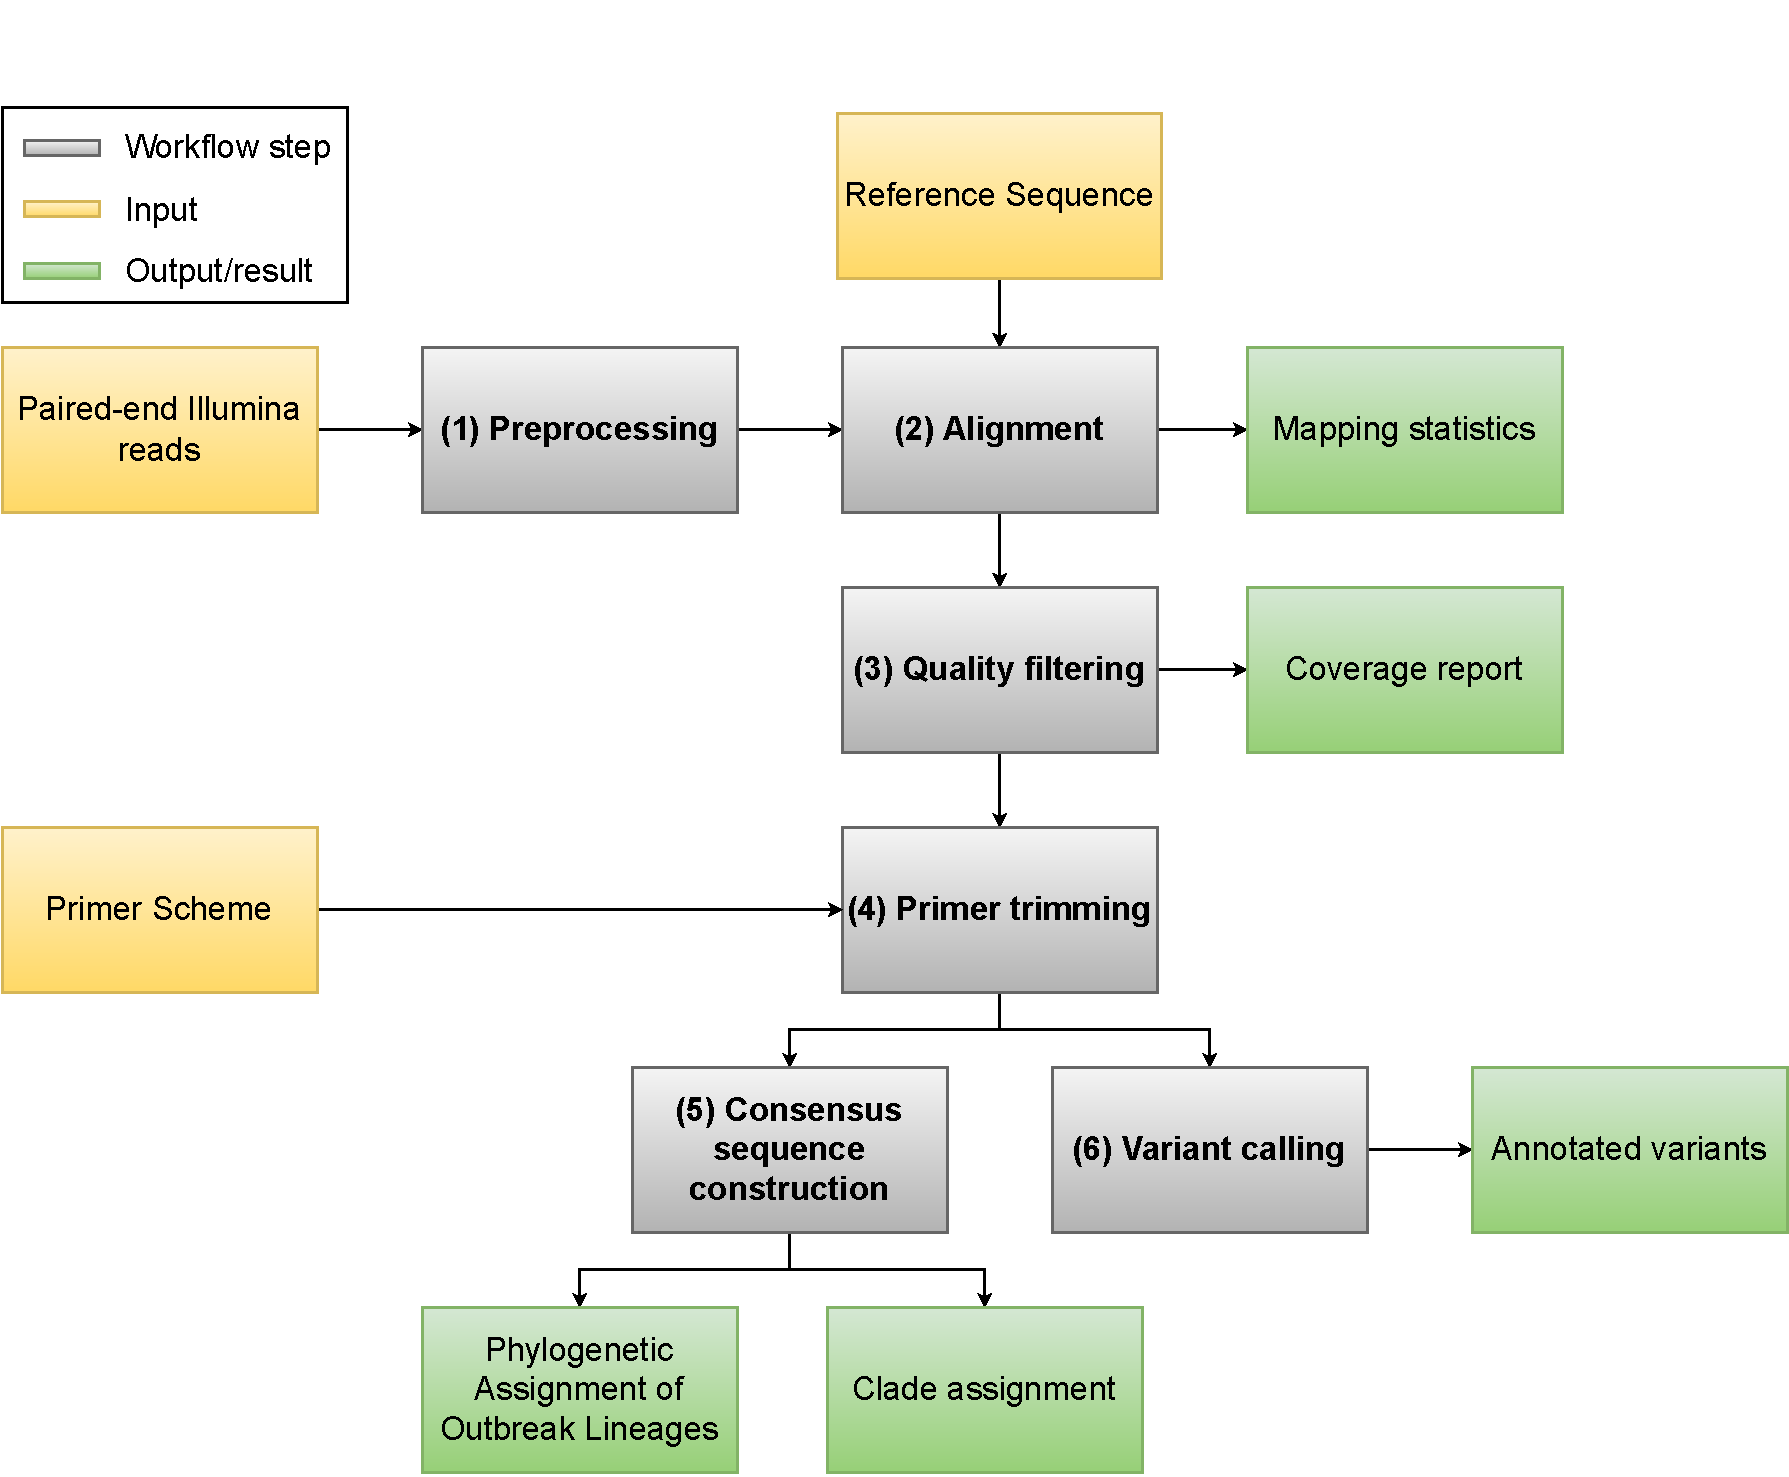
\includegraphics[width=0.95\textwidth]{media/3-sars-cov-2.pdf}
	\caption{Simplified SARS-CoV-2 analysis workflow for ampliconic Illumina-sequenced data.}
	\label{fig:3-sars-wf}
\end{figure}

This workflow is designed for the specific attributes of the \ac{SARS-CoV-2} genome, however most viral genomes can be analysed on genomic level in similar ways. Accounting for the genomic structure and composition of each virus, analysis workflows for poxviruses, avian influenza virus and foot-and-mouth disease virus are developed in this work, reusing components of the described \ac{SARS-CoV-2} workflow. The requirements for the viruses and the workflows are described below, before the developed workflows are examined.

\section{Workflow Requirements}
To account for the distinct attributes of the examined viruses, automated pipelines used to achieve whole-genome insights from raw reads must be tailored to the specific attributes of the virus being examined. The requirements for each workflow are explained below.

\subsubsection{Requirements for Poxvirus Analysis Workflow}
As explained in~\secref{sec:2-pox}, the genome of most poxviruses is bound by identical sequences located at the termini of the genome. It is shown that the size of such differs for some poxviruses like rabbitpox and vaccinia virus, while mpox, cowpox and capripoxviruses have shorter \acp{ITR}~\cite{wittek1978inverted}. For a whole-genome reconstruction from \ac{HTS}-generated reads, alignment algorithms look for the unambiguous location of a read to find the most agreed position for a complete alignment. Since there is no unambiguous position for repeated identical sequences neither in reference-based mapping approaches nor \textit{de novo} assembly, a new approach has to be used so that the two \acp{ITR} are not aligned in the same run, but separately to constitute disambiguity. Therefore, we use a method that splits the sequencing reads into two parts, separating the identical sequences and running alignment algorithms for each of the splits. To build the full-length genome, the alignments need to be ``glued'' back together. To ensure the reads to be mapped in the appropriate and not in the wrong \ac{ITR}, the reads need to be sequenced in two pools with two sequencing libraries. A similar tiling amplicon protocol has been described by Mathijs et al. and the ARTIC network for \ac{SARS-CoV-2} data~\cite{tyson2020improvements, mathijs2022robust}. \\
As a consequence, a requirement for a reference-based surveillance of the genomics of poxviruses is the availability of the primer scheme that was used for the split amplicon-based sequencing with an Illumina sequencer. Working with Illumina-generated NGS data, the workflow necessitates a quality control and trimming of the reads to remove sequencing artefacts and adapters. The \ac{BED} file containing the primers, their positions and the pool identifier is essential for the correct linking of the alignments when splitting the pipeline into two parts and merging them back together. \\
Mapping of each genome-half that each contains one \ac{ITR} requires a reference sequence, which is a compulsory workflow input. Since poxviruses have low mutation rates in general, a fixed reference sequence accounts for a nearly unambiguous mapping and consensus sequence. \\
Apart from the split approach with a masked reference sequence for alignment, the poxvirus reads can be processed in the same way as \ac{SARS-CoV-2} reads. In the \ac{SARS-CoV-2} workflow, clade and lineage assignment, with \texttt{Nextclade} and \texttt{Pangolin} respectively, work with \ac{SARS-CoV-2} specific databases. Although the tools are designed to work with the \ac{SARS-CoV-2} genome, the \texttt{Nextclade} tool is adapted and expanded to work with other viruses (mpox, Influenza A H1N1 and H3N2 HA gene, Influenza B Victoria and Yamagata HA), however not suitable for undetermined poxvirus genus members~\cite{aksamentov2021nextclade}.

\subsubsection{Requirements for AIV Analysis Workflow}
The main objectives of surveillance of \ac{AIV} on the genetic level are to get phylogenetic insights and to check for mutations or new variants that occur in the \ac{HA} and \ac{NA} proteins as a consequence of reassortment. \\
A pipeline for an avian influenza virus sample that builds a consensus sequence requires a reference sequence that it can align the NGS reads to. For an Illumina-based workflow, preprocessing is crucial to ensure reliable results working with the reads. Quality filtering and trimming must be included in the beginning of the workflow. A main caveat of many existing pipelines for \ac{AIV} genomic analysis is the user's choice of reference sequence, since it is an arbitrary selection and has a direct impact on the alignment. Another, computationally very expensive approach would be assembly which does not require a reference sequence. Since the influenza segments can have very similar regions at the segment's ends and mapping is computationally faster than assembly, a reference-guided mapping method is favoured for the analysis of \ac{AIV} samples due to the genome size and high mutation rates of \ac{AIV}. The goal is to use a reference that is representative of the sample being analysed. In the \ac{SARS-CoV-2} pipeline, it is recommended to use a reference genome from a recent \ac{SARS-CoV-2} strain. For avian influenza virus, multiple reference sequences exist depending on the strain and subtype, however this information only helps for the reference selection if the strain or subtype of the sequenced sample is known. Additionally, avian influenza viruses tend to reassort during replication and one sample may match with different possible reference sequences for the different segments. Taking a single reference for mapping, a possibly new reassortment event may not be discovered. Hence, a dynamic approach that is sensitive enough for the segmented structure of the \ac{AIV} genome is needed to pick a representative reference and to relieve the user from taking the complex choice of reference. A search tool like \texttt{VAPOR} could help identifying close reference sequences based on the input reads by looking up a large user-defined database of sequences. The diversity of \ac{HA} and \ac{NA} segments' sequences is significant enough to make it challenging to map sequenced reads to a single, full-length influenza A reference sequence. Although an approach that takes any (maybe imperfect) reference strain may be effective for the other six segments, the mapping software would frequently be unable to achieve sufficiently plausible matches for sequenced reads of the \ac{HA} and \ac{NA} segments to continue with the analysis. By introducing a method that finds the best reference sequence from a database before the actual alignment, the expensive assembly step is avoided, the user is not required to choose an arbitrary reference and mapping to a suitable reference with minimal bias can finally be performed. \\
Compared to analyses with genomes such as \ac{SARS-CoV-2} and due to the segmented structure of the \ac{AIV} genome, duplicates among the mapped reads of the \ac{AIV} sample should not be dismissed as they are in the \ac{SARS-CoV-2} workflow, but kept for maintaining a reasonable high coverage for the further analysis. Downstream analyses for phylogenetic placing are useful for the \ac{HA} and \ac{NA} genes to trace viral origins and consider relations to similar strains, as well as visual summaries of \acp{SNP} for identification of genetic variation in different regions.

\subsubsection{Requirements for FMDV Analysis Workflow}
Genomic analysis of the viral \ac{FMDV} \ac{RNA} genome requires a workflow that accounts for its high mutation rate. Aligning raw Illumina-sequenced reads requires quality control in a preprocessing step to remove sequencing platform specific adapters and dismiss reads with low quality. For alignment of the reads to construct a consensus sequence, mapping to a reference sequence or assembly are considered. Finding a representative reference sequence from a database with many sequences, for \ac{FMDV} reads this approach would regularly fail due to the very high mutation rate and ensuing large differences between the query reads and the database sequences. Therefore, a different approach to find a suitable reference sequence for mapping is required. Since the \ac{FMDV} genome is relatively short with approximately 8.3 kilobases, a \textit{de novo} assembly takes only little amount of computational resources for a run. This is due to less contigs to assemble and fewer gaps to fill during assembly, and usually more high coverage regions that facilitate the assembler to find long contigs. The overall complexity of assembly is highly reduced with short genome lengths and therefore increases efficiency of assembly.\\
A \textit{de novo} assembly of the \ac{FMDV} reads to avoid an arbitrarily chosen reference sequence with a subsequent \ac{BLAST} search in the nucleotides database is one method to find similar sequences that allow for a high-quality mapping and consensus sequence construction.\\
Additionally, the workflow should include steps for quality control, including the removal of low-quality reads and the identification and removal of potential contaminants or other sources of error. Finally, a workflow for \ac{FMDV} genomic analysis should accommodate Illumina-sequenced data and be able to scale up for working with multiple samples at a time.

\section{Workflow Development}
The developed Galaxy workflows for poxviruses, \ac{AIV} and \ac{FMDV} that account for the genomic structure of each virus and the \ac{NGS} approaches are described below.

\todo{check again all wfs and add more step descriptions}
\subsection{Poxvirus Illumina Workflow}\label{sec:pox-wf}
The newly designed Galaxy workflow for Illumina-sequenced poxvirus samples with a tiling amplicon approach is available on WorkflowHub, Dockstore and on \ac{IWC} to use on Galaxy EU. Links can be found in Supplementary~\secref{sec:apx-pox-links}. \\
This workflow is the first public pipeline for ampliconic Illumina-sequenced data that provides a ready-to-use infrastructure for genomic analysis of poxviruses with ampliconic data that were sequenced in two pools. It aims at constructing the full genome from ampliconic Illumina-sequenced reads and providing alignment files, sample-specific consensus sequences and intermediate results and reports that give insights into reads, mapping quality and mapping coverage. The pipeline is clearly shown in its structural elements in~\figref{fig:3-pox-wf}. \\ 
To account for the repeated \acp{ITR} at the ends of the poxvirus genome, the workflow is based on a tiled amplicon approach that separates the \acp{ITR} to ensure unambiguous mapping of reads. Therefore, the workflow requires the input reads in two sequencing pools that each represent one half of the genome. During the first steps, the reads of the two pools are processed individually as half genomes. Input data for the workflow are two distinct collections of reads from \textit{pool1} and \textit{pool2}, sourced from the sequencing with two libraries; the used primer scheme in \ac{BED} file format that contains an indicator for \textit{pool1} or \textit{pool2} in the \textit{SCORE} (5th) column; and a reference sequence that is used for mapping which can be retrieved from the \ac{NCBI} reference sequence database depending on the genus of the sequenced sample. 

\begin{figure}[ht!]
	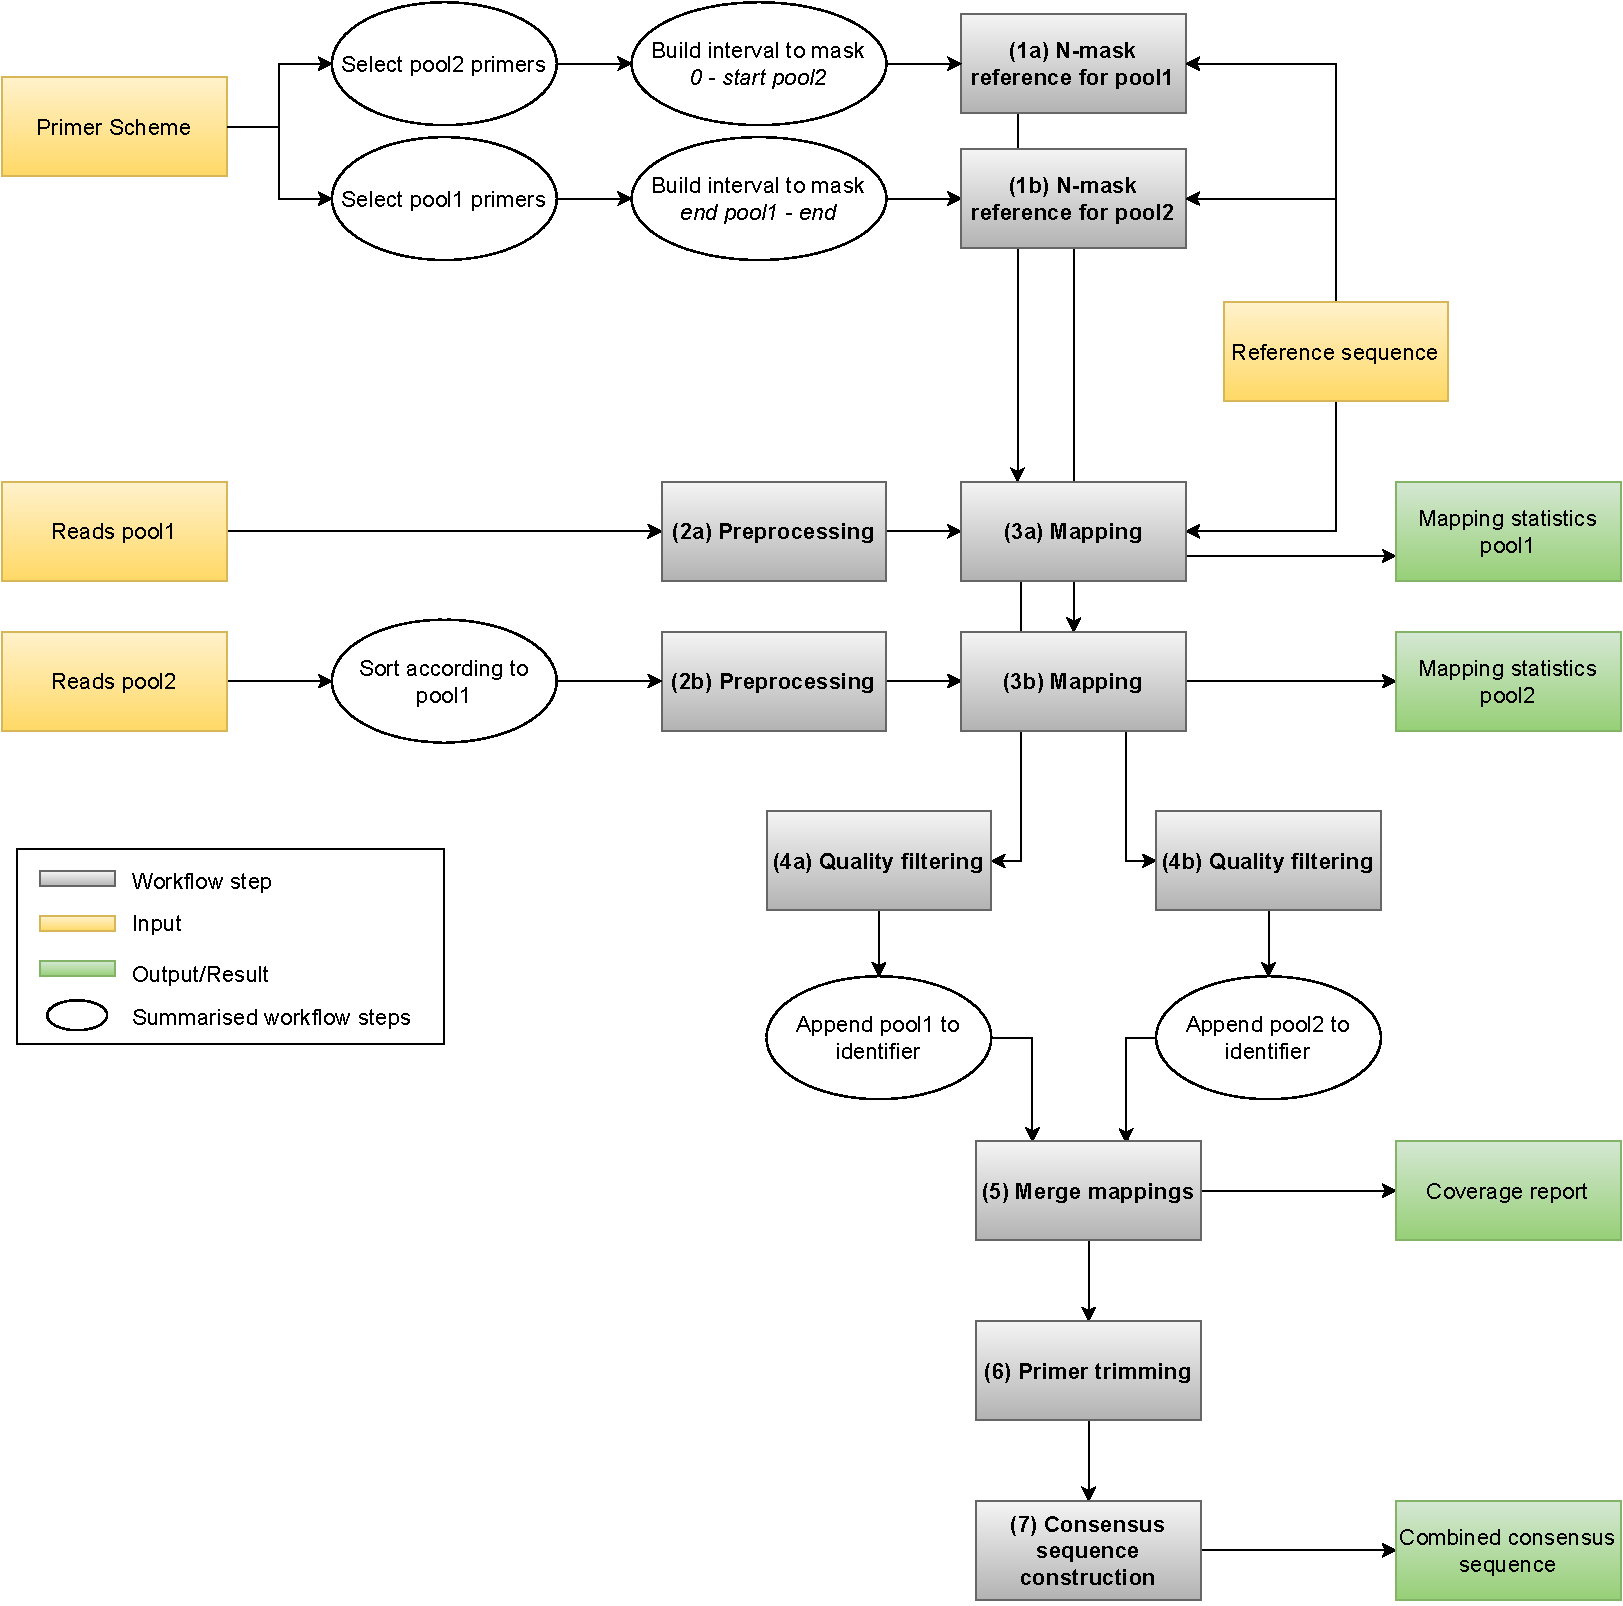
\includegraphics[width=0.92\textwidth]{media/3-pox.pdf}
	\caption{Simplified poxvirus genomic analysis workflow for ampliconic Illumina-sequenced data.}
	\label{fig:3-pox-wf}
\end{figure}

As a first step, (1) the provided reference sequence is prepared for the mapping of the two read pools. Hence, the primer scheme is needed to determine the start and end position of the two pools so that the remaining bases can be N-masked. For mapping \textit{pool1}, which accounts for the first half of primers against the full-length reference, the second half of the reference sequence is N-masked and therefore the boundaries for the remaining bases are introduced as a text parameter for further workflow logic. The N-masking of the reference starts at the minimal start position of the first primer of \textit{pool2}. If the pools and amount of primers are of similar size, this position is in the middle region of the reference sequence. It is important that this position, separating the pools, is in between the two \acp{ITR} so the individual mappings of each pool only contain one \ac{ITR}. Accordingly for the mapping of \textit{pool2}, the interval of the remaining bases is determined by taking the maximal end position of the \textit{pool1} primers and the full length of the reference sequence as an end position so that the masking of the first half can be conducted. The construction of the text parameter in the correct input format is done by multiple Galaxy-specific text-processing tools.\\
Using this approach, it is ensured that the \acp{ITR} are unambiguously mapped and coverage statistics are expressive, which would not be the case if mapping would be performed on the full-length reference and reads from the \ac{ITR} regions could be mapped to either one \ac{ITR}. \\
The poxvirus workflow is designed to process multiple samples in one run. The workflow requires the raw reads to be uploaded in two distinct collections, one for \textit{pool1} and one for \textit{pool2}, each containing the reads for potentially multiple samples. For better comparison during the workflow, the samples in the second reads pool collection are sorted by the order of how they are listed in \textit{pool1}.\\
Before mapping, (2) the reads of both pools are preprocessed with \texttt{fastp} to automatically trim Illumina-specific polyG tails of the reads and remove sequencing adapters with default settings of \texttt{fastp} to ensure further quality filtering. 
The following (3) mapping step with \texttt{BWA-MEM} takes the corresponding masked reference sequence for each genome-half as explained. A statistics report for each alignment is generated using \texttt{Samtools stats} and allows the user to inspect the mapping quality and coverage of the alignment. Next, the alignments are (4) filtered for quality using \texttt{Samtools view} to keep reads with a minimum length of 20 and only properly paired and mapped reads. Additionally, the pool identifiers (\textit{pool1/pool2}) are prepended to the sample names so that using external software to check for variants, the pool and sample identification is maintained and unambiguous for the user. In the next step, (5) the two alignments are merged while still retaining the identifiers for each sample and pool. For the full-length mapping, a coverage report is generated with \texttt{QualiMap BamQC} which allows the inspection of the \acp{ITR} and to examine the part where the mappings are merged together. The mean coverage depth is an important standard parameter when performing \ac{NGS}. It indicates how often each base occurs on average in the individual reads. For smaller segments or amplicon-based data, checking the depth of coverage in each region is crucial as it provides information on how close the sequenced sample is compared to the reference sequence that was selected for mapping. Low coverage of an alignment indicates incorrect mapping due to genetic differences. Therefore, coverage plots are provided in the workflow for each sample. \\
To prepare the alignment for consensus sequence construction, (6) primer-trimming with \texttt{iVar trim} removes the loose primer ends. The (7) consensus sequence is called with \texttt{iVar consensus} and a 50-fold minimum depth. For this step, the user can either use provided default settings (minimum quality score to count base: 20, minimum allele frequency threshold to call \ac{SNV}: 0.7, minimum allele frequency to call indel: 0.8) or enter their own values before starting the workflow. These settings yield for the minimum of 50 sequenced reads per base in coverage. With the final combined consensus sequence in FASTA format for each input sample, further downstream analyses can be started after finishing the workflow.

\subsection{AIV Illumina Workflow}\label{sec:aiv-wf}
We designed a fully automated pipeline for the analysis with a reference-based mapping approach of Illumina-sequenced paired-end reads from avian influenza samples. The workflow is integrated in the Galaxy platform and is available with all related material via links provided in Supplementary~\secref{sec:apx-aiv-links}. Furthermore, to the best of our knowledge this pipeline is the first ready-to-use workflow that uses a hybrid reference sequence for a fast mapping and provides various outputs for downstream analyses. It is designed to take one input sample at a time and quality report emitted during the workflow run, the outputs of the analysis steps can be used for any consecutive research based on the user's research objective. The \ac{AIV} workflow is outlined in~\figref{fig:3-aiv-wf}, where the nine main steps of the workflow are visualised. A link to the full workflow and its supplementary material can be found in Supplementary~\secref{sec:apx-aiv-links}. \\
One novelty of our \ac{AIV} workflow is the consideration of the different segments of the influenza virus genome in the composition of the reference sequence. After uploading paired-end reads and a reference sequence database, the workflow builds a hybrid reference from the database for each of the genome segments. The reference sequence database is described in detail in the subsequent~\secref{sec:3-aiv-ref}. If a user decides to upload their own curated references, it is important to follow the sequence identifier pattern so that the extraction of sequence identifiers in the workflow works as expected: >\textit{segment\_name$\mid$influenza\_strain$\mid$subtype$\mid$accession\_number}. Spaces must be avoided. For instance, one entry's identifier is >\textit{PB1$\mid$A/duck/Manitoba/1953$\mid$A/H10N7$\mid$KF435047.1} followed by the nucleotide sequence in the next line. 

\begin{figure}[ht!]
	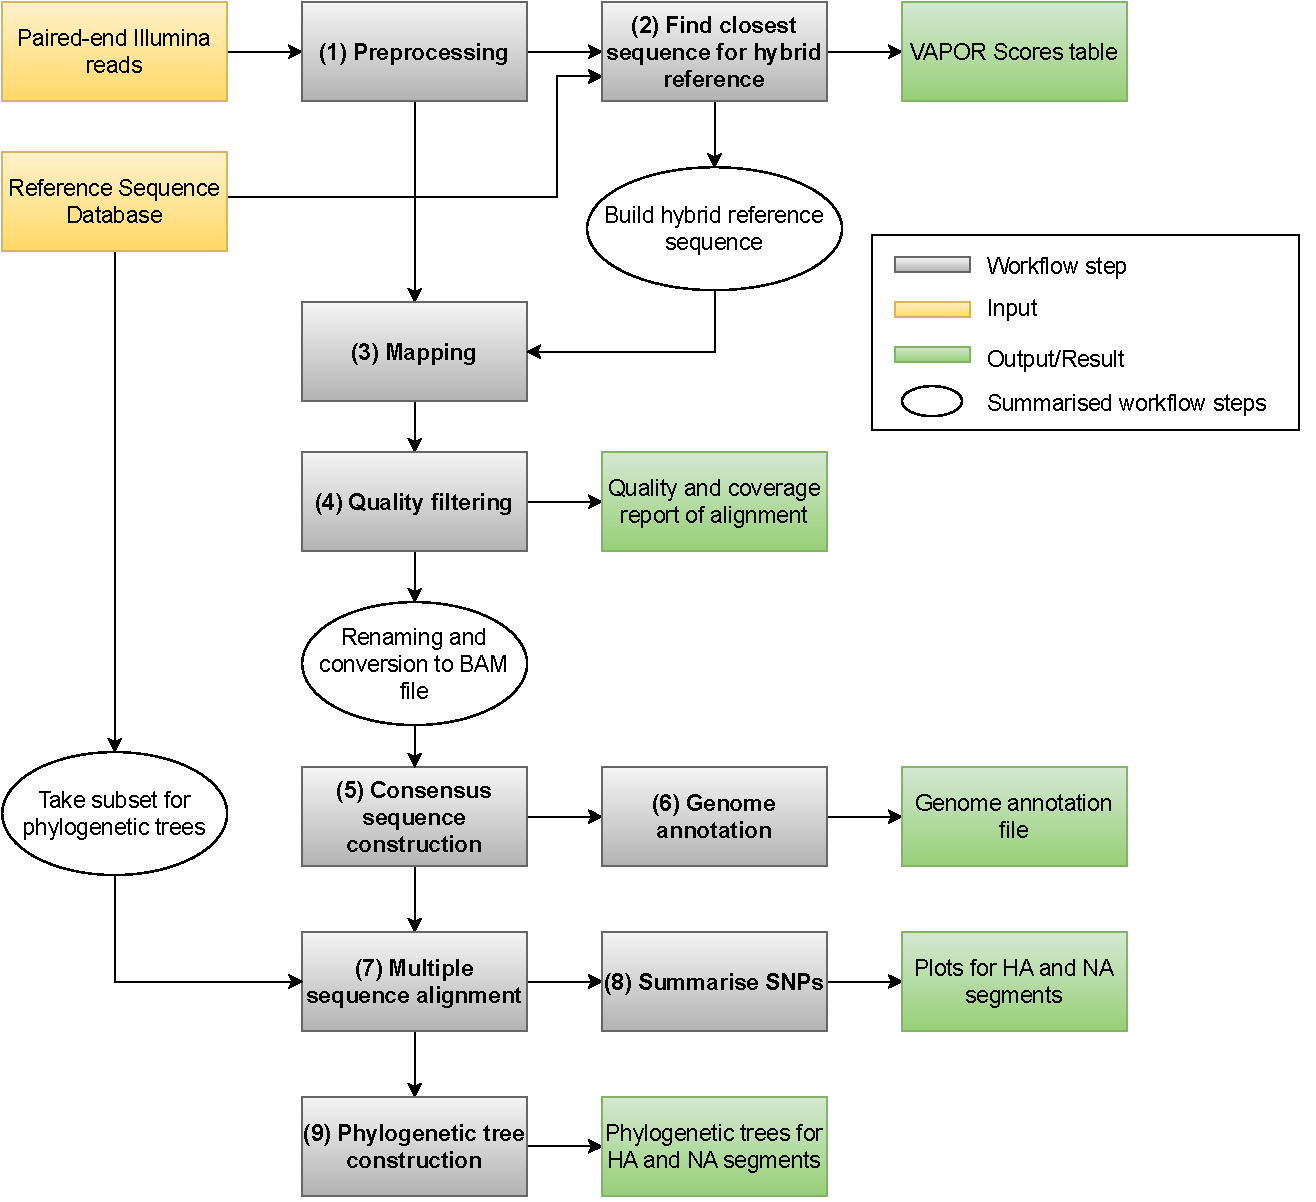
\includegraphics[width=0.88\textwidth]{media/3-aiv.pdf}
	\caption{Simplified \ac{AIV} genomic analysis workflow for Illumina-sequenced data.}
	\label{fig:3-aiv-wf}
\end{figure}

The \ac{AIV} workflow takes the reference sequences in datasets split by segment and the paired-end Illumina-sequenced reads, and an additional numeric parameter to determine the size of the produced phylogenetic tree. After (1) preprocessing of the reads with \texttt{fastp} with default quality trimming options, and additionally to dismiss reads shorter than 30 bp, filter out 5' and 3' ends with a mean quality of below Q30 (a Phred quality score of at least 30 is required) and automatic trimming of polyG tails of the Illumina reads, the database of reference sequences is used to (2) find the closest possible reference for each of the segments. The tool \texttt{VAPOR} outputs a table with a scoring based on the weighted graph construction, and should not be confused with the identity of the sequence compared to the reference. As \texttt{VAPOR} is running once per segment yet with independent inputs, the eight jobs are executed in parallel and do not depend on each other's outputs. \texttt{VAPOR} is a graph-based classifier that maps k-mers to a weighted De Bruijn graph to find sequences from a database that are as similar as possible to the query sequence~\cite{southgate2020influenza}. Benchmarking shows that it runs significantly faster than \ac{BLAST} and default configurations lead to reasonable matches similar to Mash, as long as the given sample is not very different from or novel to the provided sequences in the reference database. \\
Retrieving the highest scoring sequences from the eight \texttt{VAPOR} runs, an integral part of the workflow is to build a hybrid reference sequence used for mapping. To inspect the statistics of the graph and adapt the configuration, a table with the highest \texttt{VAPOR} scores of each run is generated and visible in the workflow history on Galaxy. \\
The hybrid reference sequence is composed of the eight segments and is used as the reference sequence in the third step of the pipeline, (3) mapping with \texttt{BWA-MEM}. The segment names in the hybrid reference genome are truncated and shortened to just the segment identifier. Mapping of the preprocessed reads against the prepared hybrid reference is run with default parameters of \texttt{BWA-MEM}. The \ac{BWA-MEM} algorithm aligns 70 to 1000 bp long reads by seeding alignments with maximal exact matches, and extending the seeds using the affine-gap Smith-Waterman algorithm~\cite{li2013aligning}. After mapping, the resulting \ac{BAM} dataset is (4) quality filtered using \texttt{Samtools view}. Reads with a minimum quality of 20 and only those that are paired and mapped in a proper pair are kept. The alignment and quality results as well as coverage statistics for each segment are reported using \texttt{QualiMap BamQC}. \\
The subsequent steps before generation of the consensus sequence from the reads alignment prepare the \ac{BAM} file and deconstruct the mapped reads into a collection of eight datasets by relabelling the elements so that (5) \texttt{iVar consensus} can perform consensus sequence construction. Per-segment consensus construction is run with a minimum quality score threshold of 20, minimum frequency threshold of 0.7, minimum depth to call consensus of 10, which does not exclude regions with smaller depth than the minimum threshold and uses N instead of ``-'' for regions with less than the minimum coverage. These settings accept any base as the consensus base for a genome position with a base calling quality of 20 or higher in order to avoid false bases that come from sequencing errors. If there is no consensus base to be found with the above criteria, an N is inserted instead. \\
To place the consensus sequence of the genome segments in a set of samples from the reference sequences to generate phylogenetic tree data, (6) a multiple sequence alignment for a user-specified number of sequences that determines the size of the resulting phylogenetic trees is done with \texttt{\acs{MAFFT}}. The consensus sequence is added using \texttt{\acs{MAFFT} add}. The multiple sequence alignment is also used for (9) a visualisation of SNPs, produced with the \texttt{snipit} tool. It provides a graphical summary of the mutations on base-resolution by comparing the consensus sequence to other close sequences from the reference database. To make the \texttt{snipit} tool available on Galaxy, a tool wrapper in XML format was written as part of this research. The link to the file is provided in Supplementary~\secref{sec:apx-wrap-links}. These sequences are selected from the top hits that resulted in the \texttt{VAPOR} run and therefore are suitable to flag up possible mutations or mis-aligned consensus bases in the consensus sequence of each influenza segment. \\
The next step in the pipeline using the consensus sequence is the (7) generation of genome annotation files with \texttt{Prokka}. Because the input sample is a viral genome, the \textit{Kingdom} parameter is set to \textit{Viruses}. With this file, open reading frames can be predicted using other tools and further downstream analyses can be started. (8) Phylogenetic trees for the \ac{HA} and \ac{NA} segments are built using \texttt{IQ-Tree}. The taxonomy of the sample segments visualised in the phylogenetic trees give insight into spatial and temporal spread of the genome. The consensus sequence from the input sample is assigned to the most likely lineage~\cite{minh2020iq}. Trees can be explored by downloading one of the standard tree formats (\textit{.nhx, .mldist} or \textit{.iqtree}) for further analysis, visualisation or using the Galaxy web-interface with visualisation tools. \\
The presented \ac{AIV} workflow avoids the computationally expensive \textit{de novo} assembly, instead uses a mapping approach with a dynamically composed reference genome of close sequences for each of the eight influenza segments. This accounts for a high quality mapping and is evaluated in~\chapref{sec:4-aiv}. To trace the individual steps and look up intermediate outputs, quality reports are emitted during the workflow process and after finishing, which can be downloaded as a PDF for each workflow run. Due to a variety of possible downstream analyses that can be interesting for a user, our workflow provides results of the individual steps which can be used with various other tools.

\subsubsection{AIV Reference Database}\label{sec:3-aiv-ref}
For reference-based mapping of the \ac{AIV} reads in the \ac{AIV} workflow, a reference sequence is required. To choose a representative sequence for each of the eight segments of the influenza genome, a database with sequences is used, split into files by segment. The reference database consists of eight FASTA files, one per segment (PB2, PB1/PB1-F2, PA/PA-X, HA, NP, NA, M1/M2, and NS1/NEP), containing multiple full-length sequences per segment.\\
The sequences were downloaded from the \ac{NCBI} Influenza Virus Database in nucleotide FASTA format. In addition, it is ensured that the 56 sequences from \ac{INSaFLU} which are provided in their reference database are part of the reference collection. Only full-length sequences with complete coding regions that include start and stop codons are used. Search results from the \ac{NCBI} Influenza Virus Database show that for some few sequences, the segment genome including start and stop codons is encoded, however includes additional sequence artefacts possibly from other segments in the front or tail. Therefore, sequences with a length of more than 105\% of the mean segment genome length according to Chauhan et al. (2022) are dismissed. Similarly, short sequences that hold less than 80\% of the mean segment nucleotide count are dismissed. This criterion ensures that a segment can be shorter than the mean length due to deletions, yet does not include sequences that are too short to reliably identify and compare with other sequences.\\
Vaccine strains and mixed subtypes are exluded from the results. Duplicate sequences are dismissed and the sequences are prepared so that the header is in the required format, does not contain spaces and has the segment name in the sequence header before the first pipe. Additionally, all sequences containing non-ACTG bases were dismissed. The remaining sequences ensure within-subtype variation of influenza strain A sequences by providing multiple sequences of the same subtype for each segment. Gene subtypes that occur only in bats as H17, H18, N10 and N11 do, are dismissed from the reference collection~\cite{tong2013new}. Due to the strict criteria, there are not always all eight segments present for one genome. The filtering criteria mentioned above are essential for maintaining the quality and reliability of the data for the \texttt{VAPOR} tool, for which the reference sequences are used as the collection to query the sample reads on. An overview of the resulting reference database and the filter criteria is provided in Supplementary~\tabref{tab:apx-aiv-ref}, as well as an overview in Supplementary~\tabref{tab:apx-aiv-ref-subtypes} of the occurrences of each subtype in the \ac{HA} and \ac{NA} genes. Since the \ac{AIV} is split into its gene segments in each dataset, the reference collection that composes subtypes from the different \ac{HA} subfamilies (1 to 18) and \ac{NA} (1 to 11) subfamilies is not required to contain all possible combinations and therefore not all subtypes are required to be present. In the \ac{AIV} workflow, the \texttt{VAPOR} tool looks for \ac{HA} sequences that are highly similar to the query reads, and provides the reference for the specific \ac{HA} subfamily sequence only from the dataset containing \ac{HA} segments. Similarly, the \ac{NA} subfamily is determined by querying the \ac{NA} dataset. This means that in the \ac{HA} \texttt{VAPOR} results and therefore in the reference used for mapping, only the \ac{HA} subfamily part (e.g. H5 from H5N10) determines the \ac{HA} subfamily. Accordingly, the \ac{NA} subfamily is derived by the most similar sequence (e.g. N8 from H3N8) within the \ac{NA} dataset. In combination, the subtype of the sample is derived (e.g. H5N8).
The reference collection with a total of 137 507 unique sequences is ready to import into a new history and publicly available on Galaxy EU. The link is provided in Supplementary~\secref{sec:apx-aiv-links}. 

\subsection{FMDV Illumina Workflow}\label{sec:fmdv-wf}
\begin{figure}[ht!]
	\centering
	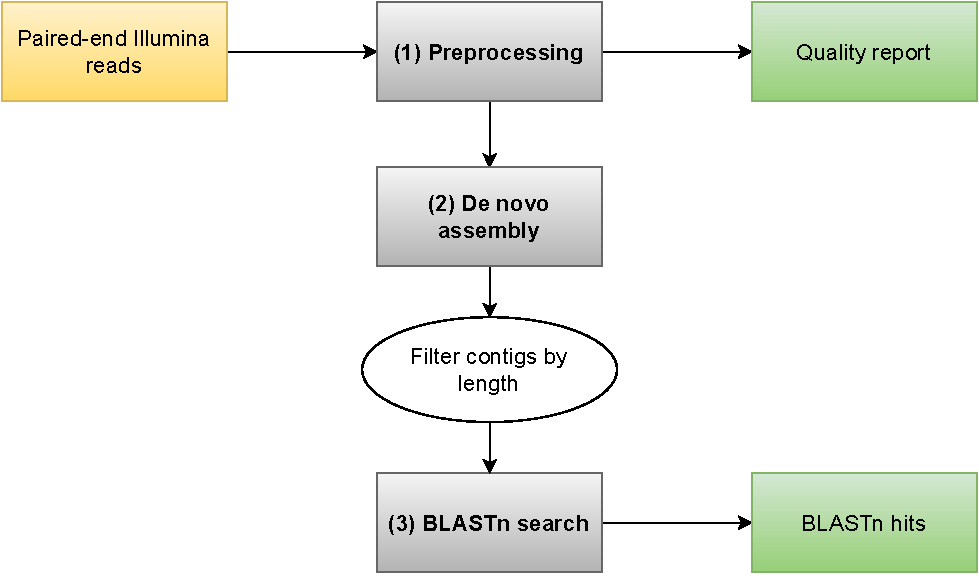
\includegraphics[width=0.9\textwidth]{media/3-fmdv-1-2.pdf}
	\caption{Simplified FMDV workflow (1/2) with \textit{de novo} assembly and BLASTn search.}
	\label{fig:3-fmdv-wf-1}
\end{figure}
\begin{figure}[ht!]
	\centering
	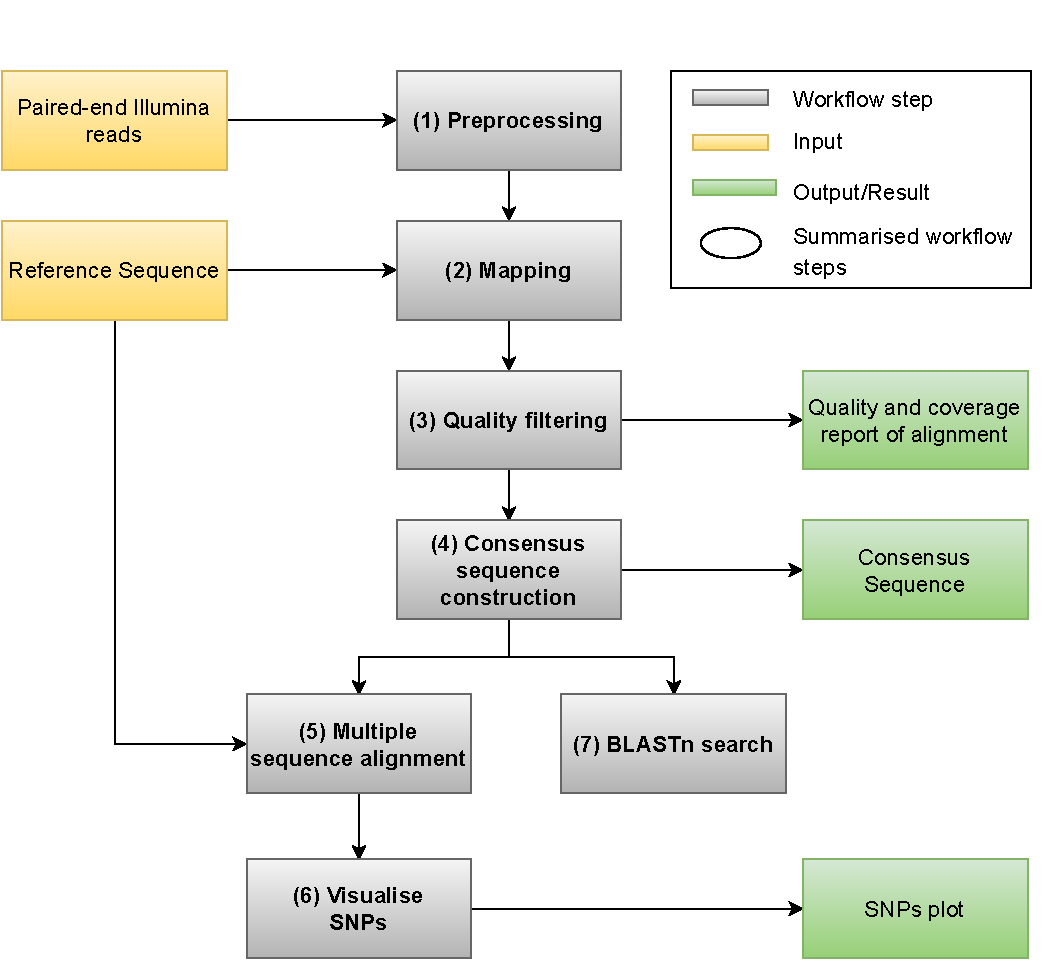
\includegraphics[width=1\textwidth]{media/3-fmdv-2-2.pdf}
	\caption{Simplified \ac{FMDV} workflow (2/2) with reference-based mapping and consensus sequence construction.}
	\label{fig:3-fmdv-wf-2}
\end{figure}

We developed a workflow for the genomic analysis of reads from Foot-and-mouth disease virus samples using Illumina sequencing technology. The workflow is split into two single workflow parts and requires the user to take action in the process of reference sequence selection. The \ac{FMDV} workflow takes multiple samples in a collection and is integrated into the Galaxy platform. Links to the two ready-to-use workflows in \textit{.ga} and \textit{.cwl} format can be found in Supplementary~\secref{sec:apx-fmdv-links}. \\

The first part of the workflow accounts for the choice of reference sequence and starts with (1) preprocessing of the reads using \texttt{fastp}. Reads shorter than 30 base pairs are discarded, and polyG tails of the Illumina reads are trimmed automatically. Default settings of \texttt{fastp} account for automatic quality filtering to remove sequencing adapters and unqualified reads by additional quality filters. Before assembly, a step to create a datastructure that allows multisample processing by the assembler is inserted to the workflow. Using the \texttt{Apply Rules} tool, a nested collection from the reads is generated, while each sample is a list containing the forward and reverse reads. This step ensures that the samples are treated separately during assembly and invoke one assembly run per sample.\\
In order to find the most similar existing sequence that can be used as a reference for mapping, this workflow first includes a \textit{de novo} assembly with \texttt{rnaviralSPAdes}. It is an assembler tailored for short \ac{RNA} viral data and was initially developed in a specific version for the assembly of \ac{SARS-CoV-2} samples. It improves the existing \texttt{SPAdes} assembler by making use of knowledge about the structure of viral \ac{RNA} genomes~\cite{meleshko2022coronaspades}. 
The \ac{FMDV} contigs, which may be varying in terms of amount of sequences and length of contig, are then (2) filtered by length to dismiss short contigs that represent only fragments of the viral genome. The cut-off is set to almost half the size of the \ac{FMDV} (minimal length 4.0 kilobases). This allows the subsequent (3) megablast search on the \ac{NCBI} NT database to find similar nucleotide genomes even in the case of co-infection of the sample or recombination within the viral genome. After the \ac{BLAST} search, the user is required to inspect the top hits, and to identify the best matching reference genome based on their own criteria such as coverage and identity. The resulting sequence that is chosen as a reference may prove plausibility of the sample or reveal the presence of other nucleic material if one of the top \ac{BLAST} results matches an unexpected virus. To avoid the automatic choice of reference selection by taking the top \ac{BLAST} match as reference for the following mapping, the workflow is split up. This implies that if a user has a different reference sequence independent of the first \ac{FMDV} workflow, the sequence analysis can start directly with the second \ac{FMDV} workflow and by uploading the reference sequence to a new Galaxy history.

The second workflow for \ac{FMDV} genomic analysis is designed for multiple raw reads in a collection that are mapped to the same reference sequence. This is useful in an outbreak scenario where a workflow user has multiple sequenced samples from the same outbreak and seeks to compare these samples with each other, identify similarities, relations and origin of the virus. However, this workflow can be used as a stand-alone pipeline without the first workflow in case the user aims to map the raw reads to a specific, arbitrarily chosen reference sequence. After uploading the reference sequence in FASTA format, identified from the megablast search and retrieved via the \ac{NCBI} upload tool (\texttt{NCBI Accession Download}) or from other sources, the workflow runs a (1) preprocessing with \texttt{fastp} to dismiss reads shorter than 30 bp and to trim polyG tails of the reads. The second step involves (2) mapping of the preprocessed reads to the reference genome using \texttt{BWA-MEM} with default configurations. This step generates a \ac{SAM} file, which is then (3) filtered for quality using \texttt{samtools}. Paired and mapped reads are kept that have a minimum quality of 20. Alignment and quality reports including coverage statistics are generated per sample using \texttt{QualiMap BamQC}. The filtered \ac{SAM} file is then used to generate a consensus sequence for each sample using the (4) \texttt{iVar consensus} tool with a minimum quality score threshold of 20, minimum frequency threshold of 0.7, minimum indel frequency threshold of 0.7 and a minimum depth of 10 to call consensus. This step allows the workflow to generate a high-quality consensus sequence for each sample, which can be used for downstream analyses, such as multiple sequence alignment and phylogenetic analysis. The resulting consensus sequences from all samples are aligned to the reference genome using (5) \texttt{\acs{MAFFT}}, and the resulting alignment is used to (6) identify and visualise \acs{SNP}s with \texttt{snipit}. The \ac{FMDV} workflow produces a summary report of the results of each step and allows the investigation in additional research with the output of each step from within the Galaxy history. 

    \chapter{Results and Workflow Evaluation}\label{chap:results}
\todoit
real-world data provided by Belgian Sciensano laboratory to test the workflow.

\section{Poxvirus Illumina Workflow}
\todoit
Samples by Sciensano by Elisabeth Mathijs

\acs{IWC} link, primer scheme.
tested with \ac{LSDV} data,
pipeline outputs on 20L70, 20L81

\subsection{LSDV Datasets 20L70 and 20L81}
\todoit

\section{AIV Workflow}\label{sec:4-aiv}
\todoit
Samples by Sciensano s4+s8, Tunesian?

point out output for downstream analyses

\subsection{AIV Datasets U2012100-n21\_S8 and U2008751-n5\_S4}
\todoit
Quality report, snipit plots, IQ-Tree for \ac{HA}/\ac{NA}, consensus reference, VAPOR scores

\section{FMDV Workflow}
\todoit
Samples by Pirbright Institute by Dr. Graham Freimanis

\subsection{FMDV Datasets ``random'' accession}
\todoit
wait for samples

\section{Workflow Profiling}
\todoit
Assembly vs. mapping

    \chapter{Discussion}\label{chap:discussion}
\todoit

\section{Contribution to the Field}
We propose three Galaxy workflows for genomic analysis of NGS-generated data for poxviruses, avian influenza virus and lumpy skin disease virus
\todoit

* Reference-based mapping pipelines\\
- dynamic choice of ref.
- avoiding assembly for large genome
- choice of tools reliable vs. new/fast
- shows that application and transfer of sars cov 2 pipelines makes sense
* Downstream analyses\\
- variant calling
- phylogeny
- gene annotation
- lineage assignment

\begin{itemize}
    \item reference-based mapping pipelines for surveillance
    \item ready-to-use, require user interaction at times to pick suitable reference sequence
    \item transfer of knowledge from SARS-CoV-2 pipelines to other viruses
    \item on Galaxy, poxvirus WF on IWC for testing and versioning
\end{itemize}

\subsubsection*{Poxvirus Analysis}
\ac{LSDV} interesting for all poxviruses and adjustable due to \acp{ITR} and tiled-amplicon approach \\
further pox viruses, pipelines can be more or less easily applied/adjusted \\
single sample vs. multi sample (reality check, what is needed? maybe multiple samples from one outbreak)


\subsubsection*{Avian Influenza Virus Analysis}
\ac{AIV} downstream - everything is possible. Highlight key minor assets that indicate adaption to mammals -> databases needed to check against, detect mutation of isolates? \\
Generally: annotate on amino acid layer (most information) \\

AIV: Choice of reference (issue of reference ambiguity), why not BLAST or lookup in GISAID with many hundereds of thousands of RNA virus genomes; \\
AIV: Alternatives, such as read classification by mapping to a large database of influenza sequences and subsequent de novo assembly can help to resolve this issue, such pipelines are often complex, slow, and require expertise that is not necessarily available in routine
surveillance or public health laboratories. Secondly, even if bioinformatics pipelines are chosen judiciously, sequences of zoonotic origin may fail to be identified, resulting in a dataset that appears to below coverage, missing segments, or missing potential future pandemic reassortments. Furthermore, even with recent assembly programs, misassembly can occur.

However using an optimal reference is ideal, since for later advanced applications, such as transmission events, or study of intra-host variation, the closest possible reference may be necessary. Whilst BLAST performed well for individual read classification, it is often too slow for general application. With regards to de novo assembly, in the cases where not enough initial data exists to assemble fragments, mapping allows analysis of limited fragments. Furthermore, assembly of virus genomes can be slow, often taking several days for a single sample when contaminant reads are present.

Make phylogenetic trees publicly accessible, not one sample per strain but in high resolution and greater details, strains from different countries,
single sample vs. multi sample (reality check, what is needed? maybe multiple samples from one outbreak) 


\subsubsection*{Foot-and-mouth Disease Virus Analysis}
If the goal in a broad and rapid surveillance is a high number of sample throughput and analysis, assembly is too cost and time sensitive for large viral genomes. However small viral genomes such as FMDV perform reasonably faster in a de novo assembly than larger DNA genomes and achieve sufficiently good results. Long assembled contigs can be used for choosing a good, representative reference sequence that can be used for mapping. BLAST provides a large database however needs regular updates to deliver current hits and proper surveillance, also relevant for downstream/phylogeny.
Workflow in two parts requires knowledge and interaction by the user -> error prone?

Nevertheless this is the most suitable approach for high resolution genomic analysis, as a direct mapping fails due to not fitting reference sequences

--------------\\
Workflows that solve common problems, provide useful information, are user-friendly, customisable, extendable

limitations \\

``The high sensitivity of the \ac{NGS} technology ensures that major kinds of viral pathogens in mixed samples can be detected.''
One strength of \ac{NGS} is that it can be used to detect emerging viral diseases with a high genetic variation. Like \ac{AIV}. Since it can analyse a full sequence instead of targeting a specific gene. -> makes sense to use virus-specific primers for \ac{PCR} or \ac{NGS} 

``Comparison of the whole genome sequences of recent \ac{LSDV} isolates from the 2015–2016 epidemic in southern Europe revealed only a limited number of point mutations between the isolates'' \ac{WGS} is essential to capture all genetic variation at once

In sequencers, false positive variants (\ac{FPV}) must be avoided (happens when too many amplification cycles are made)

BWA-MEM vs. BWA-MEM2 for small viral genomes: no big speed gain, error-prone as a new tool. preferably stick to known tools in Galaxy that are proved to work well and have a maintenance

-> caveat of tools with small development teams: abundance of technological advancements or error solving, but dependence on the reliability -> choose established software

% Efficiency: Assembly vs. Mapping; efficiency
% Kraken2 vs. VAPOR; 
% Efficiency: LoFreq vs. iVar consensus; both consensus identification methods using the same site-specific depth threshold

% building index is expensive (BWT)

FMDV: This user-involving method ensures that the consensus sequence for each sample is generated based on the closest available reference sequence, which can improve the accuracy and reliability of the final assembly. 

\section{Limitations}
\todoit
\begin{itemize}
    \item Illumina seq. data
    \item VAPOR 
    \item amplicon scheme for poxviruses
    \item mapping-based approach reaches its limits for FMDV -> requires user interaction
    \item AIV and FMDV not tested with many samples
\end{itemize}


\section{Future Directions}
\todoit
\begin{itemize}
    \item validate with more samples/tests
    \item extend to more NGS datatypes
    \item replace tools with faster/newer tools (if available, stable and reliable on Galaxy)
    \item apply to more viruses
    \item enhance surveillance, write more training material, use pipelines in production
\end{itemize}

further validation and improvement of the developed pipelines, application to other viral livestock diseases, integration with existing surveillance systems; expand the \ac{VETLAB} network to entitle even more professionals to professionally analyse their samples.
more testing, more training material

workflows offer many possible directions for downstream analysis that could be integrated into the main workflows if needed:

* consensus sequence for each segment -> compare consensus sequence to others can help identify outbreaks and patterns of transmission, get more insights how the virus spreads and its evolution
* Prokka annotation file. Predict the protein coding regions of the virus, to understand the function of the viral proteins and how they interact with host cells
* SNPs relative to the reference sequence
* \ac{MSA} and phylogenetic tree for broad or detailed phylogenetic analysis and understand evolutionary relationships between the sample and other strains. could also use clusters or subtypes within the sample. make trees available so that new isolates can be immediately arranged
* more visualisation of the data
* long-term objective: build public high-resolution databases to enable researchers to detect mutation of an isolate. this is crucial for a global surveillance system to work.
* develop workflows for the same purpose that work with other NGS sequencing data (ONT, PacBio etc.)

fine-tune settings of individual tools, improve quality of tools (VAPOR)
    \chapter{Conclusion}\label{chap:conclusion}
Whole-genome sequencing data provide valuable information on viral samples of emerging livestock diseases. Automated pipelines, accessible on the community-based and open-sourced Galaxy platform, solve the complex task of reconstructing the consensus sequence from raw read data. The developed workflows carefully take into account virus-specific characteristics for high-quality genomic analysis, while relying on the concept of reference-based mapping instead of error-prone and computationally expensive \textit{de novo} assembly. The decision on a representative reference is integrated into each workflow by database searches. Especially for \ac{AIV}, reassortment events occurring in the individual gene segments challenge the choice of appropriate reference sequence, which makes it difficult to agree on a single sample that fits in all eight segments. Relying directly on raw read data rather than assembled contigs and allowing the backtracing to the raw data, integrating the dynamic reference selection based on a classification search in a large database goes beyond current influenza surveillance pipelines.\\
Poxviruses are attributed with identical repeated regions within the genome where unambiguous alignment regularly fails and in order to solve this challenge, a tiling amplicon approach is used. It requires sequencing of the sample in two pools and executes mapping in two steps to separate the ambiguous positions.\\
For shorter viral genomes such as \ac{FMDV}, we showed that \textit{de novo} assembly is reasonably faster than for large \ac{DNA} genomes and serves as a starting point for a reference search for mapping. It involves the user deciding on a reference sequence by reviewing the megablast search results. This way, possibly unexpected contamination or coinfection in the sample can be detected. While all three approaches are highly specific for the viral attributes, they share common goals with in terms of lineage identification and allelic variant extraction, and rely on approved concepts used in other existing pipelines like such for genomic sequence analysis of \ac{SARS-CoV-2}.\\
Combining steps of proper preprocessing and filtering to reduce misalignments and the incorporation of sequencing errors into the alignment, downstream analysis based on alignment files and consensus sequence like variant calling, phylogenetic embedding and gene annotation are missing concepts in the workflows. Still, the workflows serve as starting points for more, specialised surveillance efforts of important notifiable viral livestock diseases.

    \bibliographystyle{ieeetr}
    \bibliography{bib/bib}
    \addcontentsline{toc}{chapter}{Bibliography}
    \newpage
    \chapter*{Appendix}
\label{chap:appendix}

\vspace*{-16pt}
\refstepcounter{section}
\section*{\thesection \quad Links to Workflows and Additional Materials}
\hspace*{-18pt}All workflows in Galaxy-specific GA and CWL formats are available on GitHub:\\
\url{https://github.com/kciy/msc-thesis/tree/main/workflows/}

\refstepcounter{subsection}
\subsection*{\thesubsection \quad Poxvirus Workflow}
\label{sec:apx-pox-links}

\begin{itemize}
	\setlength{\itemsep}{-0.4cm}
	\item Galaxy EU:\\
	\url{https://usegalaxy.eu/u/vyetoria/w/pox-virus-illumina-amplicon}
	\item GitHub Intergalactic Workflow Commission:\\
	\url{https://github.com/galaxyproject/iwc/tree/main/workflows/virology/pox-virus-amplicon}
	\item WorkflowHub:\\
	\url{https://workflowhub.eu/workflows/439}
	\item Dockstore:\\
	\url{https://dockstore.org/workflows/github.com/iwc-workflows/pox-virus-amplicon/main:main?tab=info}
	\item Galaxy Training Material: \todoit
	\item Galaxy history with workflow test run (\ac{LSDV} samples 20L70 and 20L81):\\
	\url{https://usegalaxy.eu/u/vyetoria/h/pox-virus-illumina-amplicon-sample-lsdv} 
\end{itemize}

\refstepcounter{subsection}
\subsection*{\thesubsection \quad Avian Influenza Virus Workflow}
\label{sec:apx-aiv-links}

\begin{itemize}
	\setlength{\itemsep}{-0.4cm}
	\item Galaxy EU:\\
	\url{https://usegalaxy.eu/u/vyetoria/w/aiv-illumina-analysis}
	\item Reference Database:\\
	\url{https://usegalaxy.eu/u/vyetoria/h/aiv-reference-sequences}
	\item Galaxy Training Material:\\
	\url{https://training.galaxyproject.org/training-material/topics/variant-analysis/tutorials/aiv-analysis/tutorial.html}
	\item Galaxy history with workflow test run (H4N6 sample):\\
	\url{https://usegalaxy.eu/u/vyetoria/h/aiv-seq-analysis-test-h4n6}
	\item Galaxy history with workflow test run (H5N8 sample):\\
	\url{https://usegalaxy.eu/u/vyetoria/h/aiv-seq-analysis-test-h5n8}
\end{itemize}

\refstepcounter{subsection}
\subsection*{\thesubsection \quad Foot-and-mouth Disease Virus Workflows}
\label{sec:apx-fmdv-links}

\begin{itemize}
	\setlength{\itemsep}{-0.4cm}
	\item Part 1 (\textit{De novo} assembly and BLASTn search) Galaxy EU:\\
	\url{https://usegalaxy.eu/u/vyetoria/w/fmdv-sequence-analysis-part-1-assembly-and-blastn-search}
	\item Part 2 (Mapping and consensus sequence construction) Galaxy EU:\\
	\url{https://usegalaxy.eu/u/vyetoria/w/fmdv-sequence-analysis-part-2-mapping-consensus}
	\item Galaxy history with workflow 1 test run (SRR17960053, SRR18751245, SRR18685689 and SRR9328470):\\
	\url{https://usegalaxy.eu/u/vyetoria/h/fmdv-sequence-analysis-1-2}
	\item Galaxy histories of workflow 2 test runs:
	\begin{itemize}
		\setlength{\itemsep}{-0.4cm}
		\vspace*{-0.4cm}
		\item SRR17960053 (Asia-1 sample):\\
		\url{https://usegalaxy.eu/u/vyetoria/h/fmdv-seq-analysis-2-2-asia-1}
		\item SRR18751245 (A sample):\\
		\url{https://usegalaxy.eu/u/vyetoria/h/fmdv-seq-analysis-2-2-a}
		\item SRR18685689 (SAT-1 sample):\\
		\url{https://usegalaxy.eu/u/vyetoria/h/fmdv-seq-analysis-2-2-sat-1}
		\item SRR9328470 (SAT-2 sample):\\
		\url{https://usegalaxy.eu/u/vyetoria/h/fmdv-seq-analysis-2-2-sat-2}
	\end{itemize}
\end{itemize}


\refstepcounter{section}
\section*{\thesection \quad Reference Collection for AIV Workflow}

\setlength{\tabcolsep}{8pt}
\renewcommand{\arraystretch}{1.3}
\begin{table}[ht!]
	\centering
	\begin{tabular}{@{}llcccccc@{}}
	\hline
					 &                   & \multicolumn{1}{l|}{}                                                           & \multicolumn{2}{c|}{\textbf{Filter criteria \textsuperscript{1}}}                                                                                                                    & \multicolumn{3}{c}{\textbf{Reference collection}}                                                                                                                                                \\ \hline
	\multicolumn{2}{l}{Segment} & \multicolumn{1}{l|}{Length \textsuperscript{2}} & \multicolumn{1}{l}{\begin{tabular}[c]{@{}l@{}}Minimum\\ length\end{tabular}} & \multicolumn{1}{l|}{\begin{tabular}[c]{@{}l@{}}Maximum\\ length\end{tabular}} & \multicolumn{1}{l}{\begin{tabular}[c]{@{}l@{}}\# of\\ sequences\end{tabular}} & \multicolumn{1}{l}{Length range} & \multicolumn{1}{l}{\begin{tabular}[c]{@{}l@{}}Mean\\ length\end{tabular}} \\ \hline
	1                & PB2               & \multicolumn{1}{c|}{2 316}                                                      & 1 945                                                                          & \multicolumn{1}{c|}{2 432}                                                      & 17 714                                                                        & 2 244 - 2 417                      & 2 306.7                                                                     \\
	2                & PB1               & \multicolumn{1}{c|}{2 316}                                                      & 1 945                                                                          & \multicolumn{1}{c|}{2 432}                                                      & 17 355                                                                        & 2 265 - 2 414                      & 2 304.9                                                                     \\
	3                & PA                & \multicolumn{1}{c|}{2 208}                                                      & 1 766                                                                          & \multicolumn{1}{c|}{2 318}                                                      & 17 569                                                                        & 1 905 - 2 275                      & 2 192.4                                                                     \\
	\textbf{4}       & \textbf{HA}       & \multicolumn{1}{c|}{\textbf{1 752}}                                             & \textbf{1 401}                                                                 & \multicolumn{1}{c|}{\textbf{1 840}}                                             & \textbf{20 753}                                                               & \textbf{1 659 - 1 805}             & \textbf{1 717.5}                                                            \\
	5                & NP                & \multicolumn{1}{c|}{1 540}                                                      & 1 232                                                                          & \multicolumn{1}{c|}{1 617}                                                      & 16 024                                                                        & 1 440 - 1 616                      & 1 529.9                                                                     \\
	\textbf{6}       & \textbf{NA}       & \multicolumn{1}{c|}{\textbf{1 434}}                                             & \textbf{1 147}                                                                 & \multicolumn{1}{c|}{\textbf{1 506}}                                             & \textbf{17 646}                                                               & \textbf{1 308 - 1 498}             & \textbf{1 418.8}                                                            \\
	7                & MP                & \multicolumn{1}{c|}{1 002}                                                      & 801                                                                            & \multicolumn{1}{c|}{1 052}                                                      & 14 684                                                                        & 979 - 1 047                        & 1 001.0                                                                     \\
	8                & NS                & \multicolumn{1}{c|}{865}                                                        & 692                                                                            & \multicolumn{1}{c|}{908}                                                        & 15 762                                                                        & 752 - 907                          & 860.9                                                                       \\ \hline
	\multicolumn{8}{l}{\begin{tabular}[c]{@{}l@{}}\textsuperscript{1} Minimum cutoff length is 80\% of segment length, maximal cutoff length is \\105\% of segment length.\\\textsuperscript{2} For strain A/swine/Iowa/18Tosu0505/2018(H1N1)~\cite{chauhan2022overview}.\\\end{tabular}}                                                
	\end{tabular}
	\caption{Summary of reference collection obtained from search criteria on the NCBI Influenza Virus Database.}
 \label{tab:apx-aiv-ref}
\end{table}
\newpage
\setlength{\tabcolsep}{10pt}
\renewcommand{\arraystretch}{1.3}
\begin{table}[ht!]
	\centering
	\begin{tabular}{@{}lcclcc@{}}
	\hline
	\textbf{\begin{tabular}[c]{@{}l@{}}HA\\Subtype\end{tabular}}  & \textbf{\begin{tabular}[c]{@{}l@{}}\# of HA\\ sequences\end{tabular}}  & \textbf{\begin{tabular}[c]{@{}l@{}}\# of NA\\ sequences\end{tabular}}  & \textbf{\begin{tabular}[c]{@{}l@{}}NA\\Subtype\end{tabular}}  & \textbf{\begin{tabular}[c]{@{}l@{}}\# of HA\\ sequences\end{tabular}}  & \textbf{\begin{tabular}[c]{@{}l@{}}\# of NA\\ sequences\end{tabular}}  \\ \hline
	\textbf{H1}  & 779          & 787          & \textbf{N1}  & 4 317        & 3 797        \\
	\textbf{H2}  & 512          & 450          & \textbf{N2}  & 6 346        & 5 419        \\
	\textbf{H3}  & 1 857        & 1 724        & \textbf{N3}  & 1 585        & 1 387        \\
	\textbf{H4}  & 1 561        & 1 520        & \textbf{N4}  & 344          & 304          \\
	\textbf{H5}  & 5 199        & 4 345        & \textbf{N5}  & 523          & 442          \\
	\textbf{H6}  & 1 817        & 1 808        & \textbf{N6}  & 2 454        & 2 360        \\
	\textbf{H7}  & 1 898        & 1 655        & \textbf{N7}  & 838          & 761          \\
	\textbf{H8}  & 169          & 155          & \textbf{N8}  & 2 255        & 2 077        \\
	\textbf{H9}  & 3 530        & 2 835        & \textbf{N9}  & 1 260        & 1 092        \\
	\textbf{H10} & 866          & 851          & \textbf{N10} & 0            & 0            \\
	\textbf{H11} & 749          & 672          & \textbf{N11} & 0            & 0            \\
	\textbf{H13} & 370          & 310          &              &              &              \\
	\textbf{H14} & 42           & 38           &              &              &              \\
	\textbf{H15} & 15           & 12           &              &              &              \\
	\textbf{H16} & 225          & 177          &              &              &              \\
	\textbf{H12} & 337          & 266          &              &              &              \\
	\textbf{H17} & 0            & 0            &              &              &              \\
	\textbf{H18} & 0            & 0            &              &              &              \\ \hline
	\end{tabular}
	\caption[AIV reference collection by HA and NA subtypes.]{Amount of sequences per HA and NA gene dataset of reference sequences, divided by 18 HA and 11 NA subtypes present in the AIV reference database, retrieved from NCBI Influenza Virus Database. Subtypes H17, H18, N10 and N11 are excluded for irrelevance in livestock (H17N10 and H18N11 only known in bats~\cite{tong2013new}).}
\label{tab:apx-aiv-ref-subtypes}
\end{table}

\begin{figure}
	\refstepcounter{section}
	\section*{\thesection \quad Results of H4N6 and H5N8 Samples for AIV Workflow}
	\centering
	\begin{subfigure}[b]{1.1\textwidth}
		\hspace*{-50pt}
		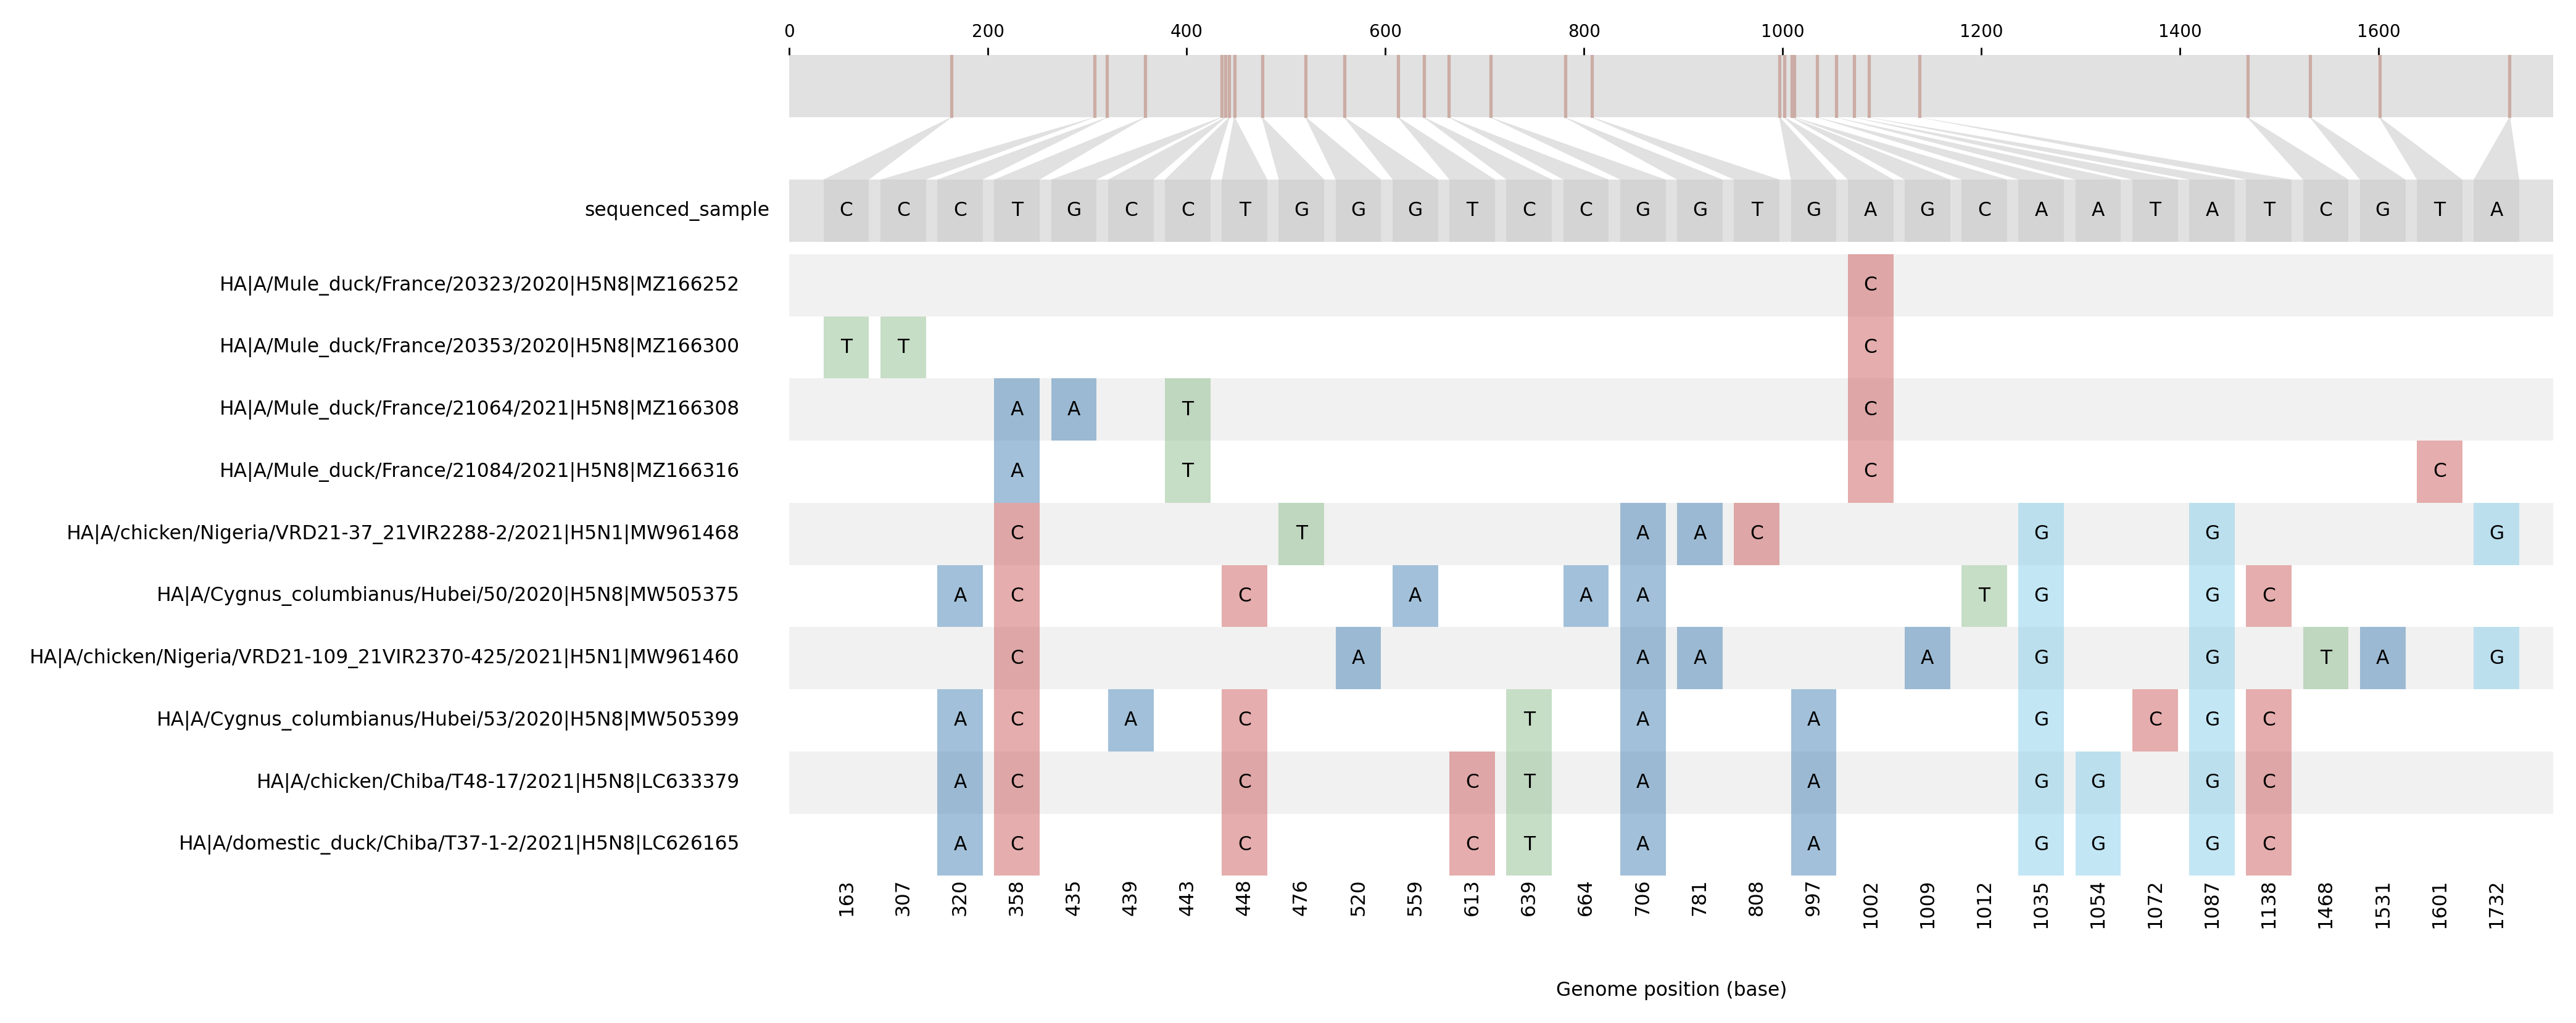
\includegraphics[width=1.0\textwidth]{media/4-aiv-snipit-s8-4-ha.png}
		\caption{SNPs of HA gene of H5N8 sample.}
		\label{fig:apx-aiv-snipit-s8-ha}
	\end{subfigure}
	\\
	\vspace*{20pt}
	\begin{subfigure}[b]{1.0\textwidth}
		\hspace*{-40pt}
		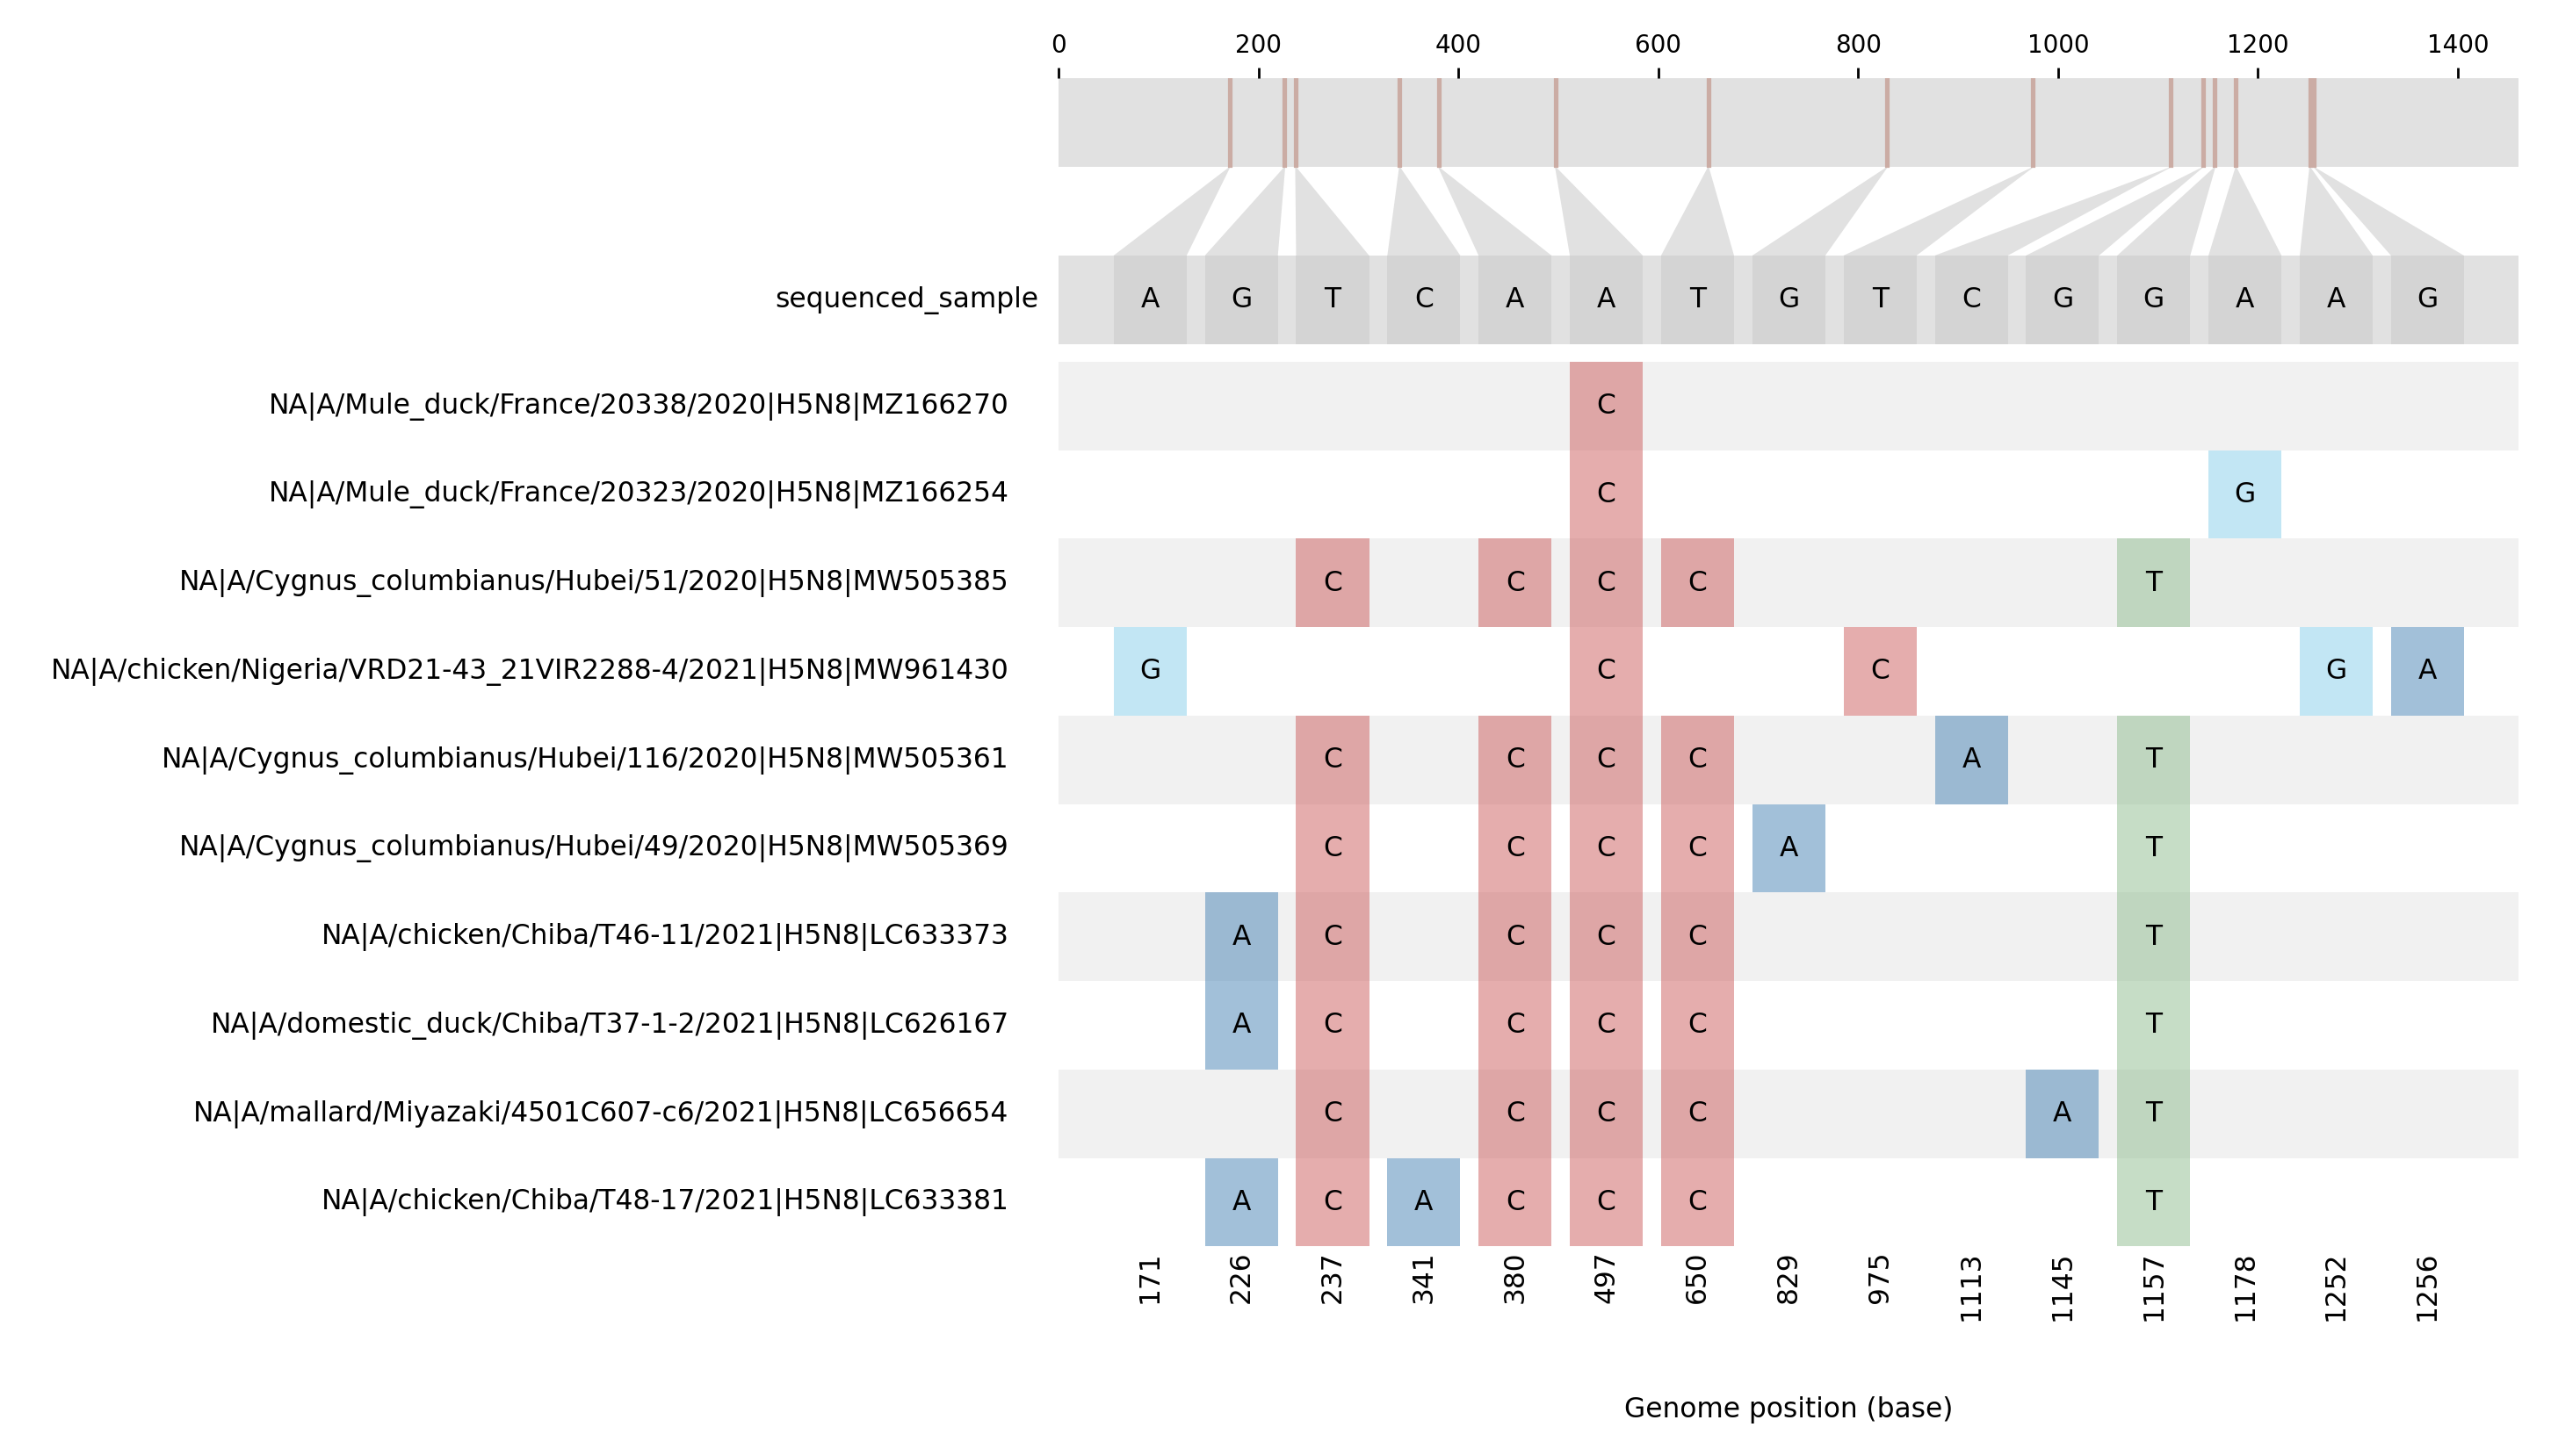
\includegraphics[width=1.0\textwidth]{media/4-aiv-snipit-s8-6-na.png}
	\caption{SNPs of NA gene of H5N8 sample.}
	\label{fig:apx-aiv-snipit-s8-na}
	\end{subfigure}
	\caption[Visual summaries of SNPs in H5N8 sample.]{Visual summaries of SNPs in H5N8 sample. The consensus sequence of the gene is the reference at the top of each plot.}
\label{fig:apx-aiv-snipit-s8}
\end{figure}

% todo: look that this is on an even page (read position numbers or rotate)
\begin{sidewaysfigure}
    \centering
    \subfloat[SNPs of HA gene of H4N6 sample.]{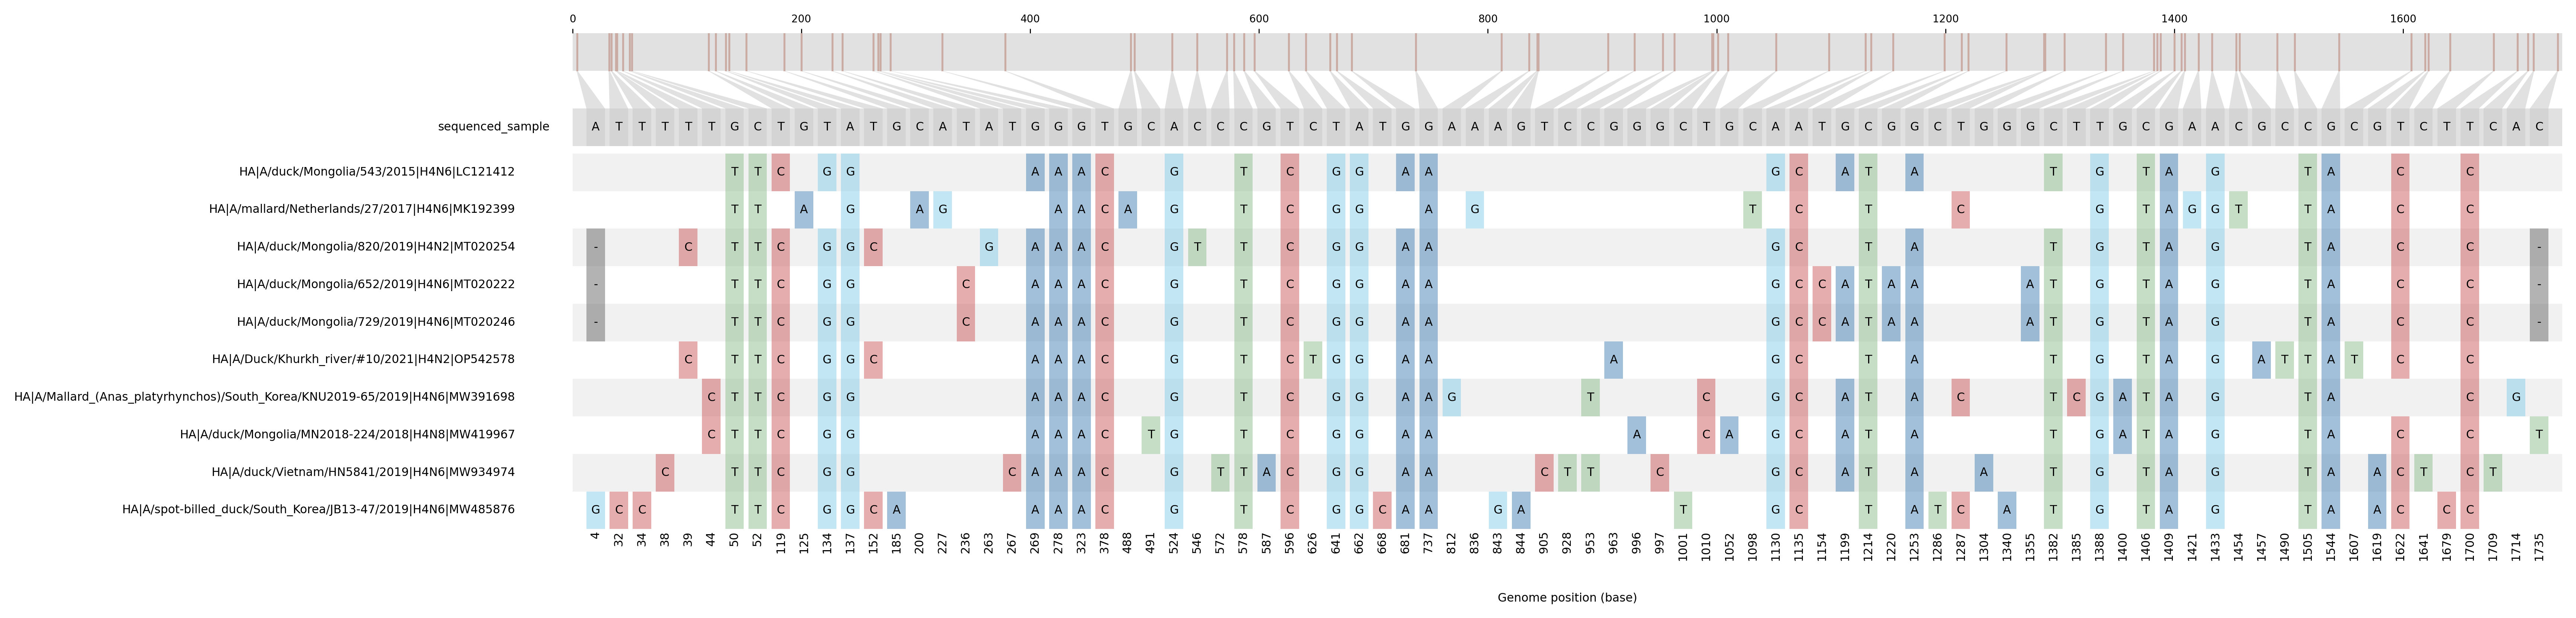
\includegraphics[width=1.0\textheight]{media/4-aiv-snipit-s4-4-ha.png}\label{fig:apx-aiv-snipit-s4-ha}} \\
    \subfloat[SNPs of NA gene of H4N6 sample.]{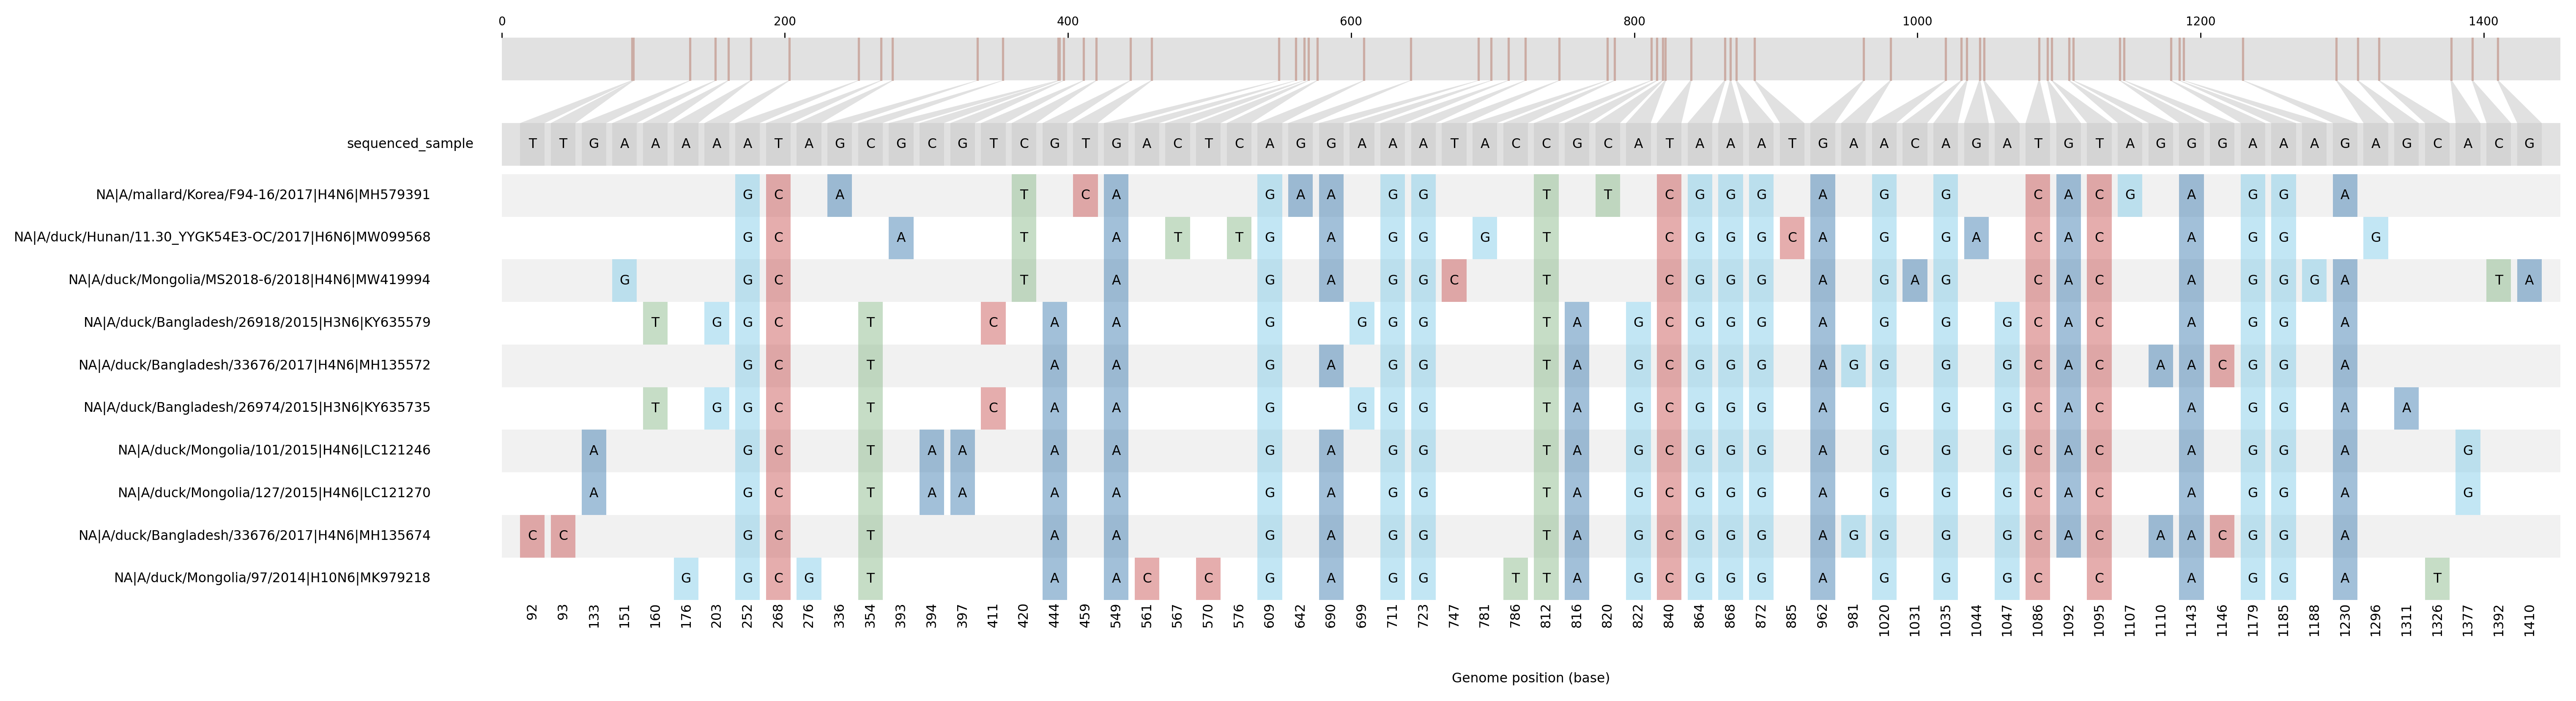
\includegraphics[width=1.0\textheight]{media/4-aiv-snipit-s4-6-na.png}\label{fig:apx-aiv-snipit-s4-na}}
    \caption[Visual summaries of SNPs in H4N6 sample.]{Visual summaries of SNPs in H4N6 sample. The consensus sequence of the gene is the reference at the top of each plot.}
\label{fig:apx-aiv-snipit-s4}
\end{sidewaysfigure}

\begin{figure}
    \centering
    \begin{subfigure}[]{0.5\textheight}
        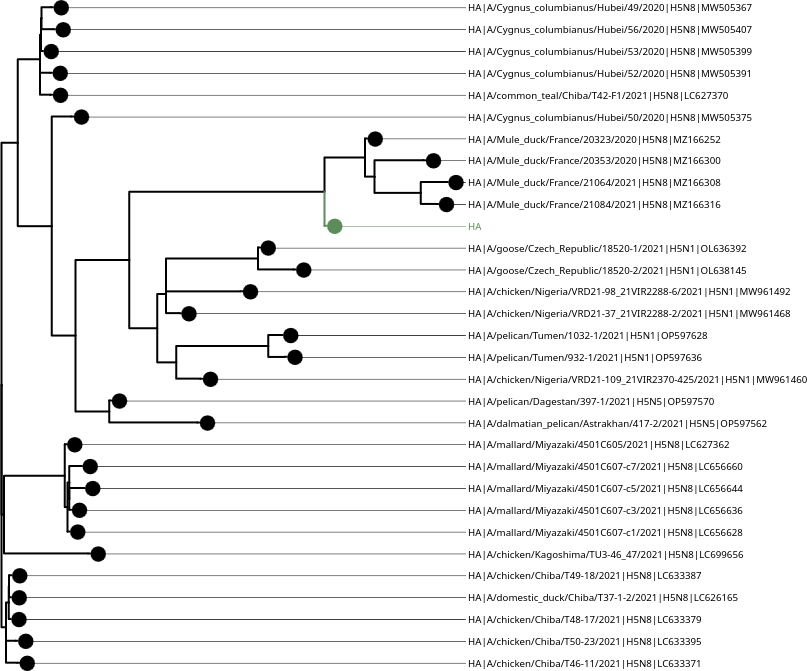
\includegraphics[width=1.0\textwidth]{media/4-aiv-s4-tree-ha.png}
        \caption{Phylogenetic tree of HA gene of H4N6 sample.}
		\label{fig:apx-aiv-trees-s4-ha}
    \end{subfigure} \\
	\vspace*{20pt}
    \begin{subfigure}[]{0.5\textheight}
        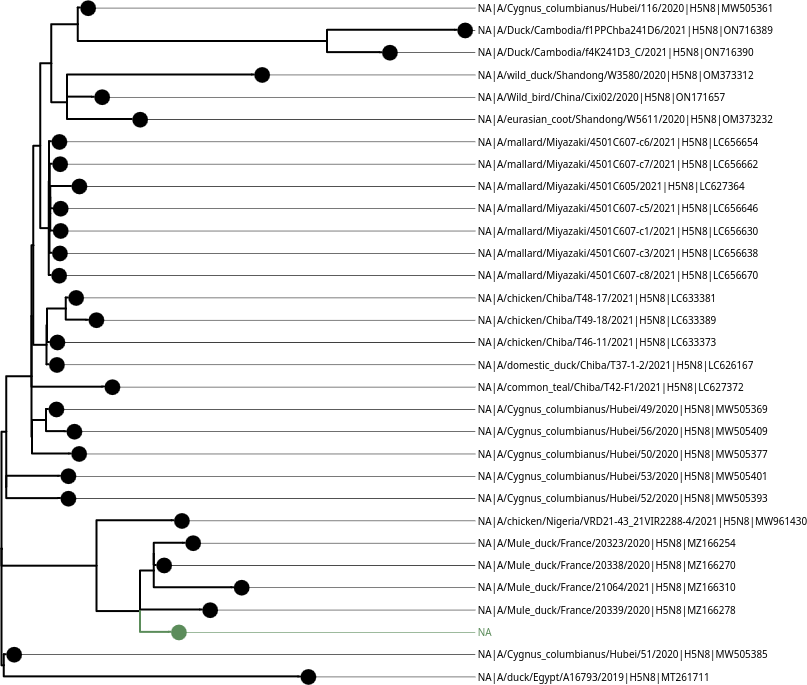
\includegraphics[width=1.0\textwidth]{media/4-aiv-s4-tree-na.png}
        \caption{Phylogenetic tree of NA gene of H4N6 sample.}
		\label{fig:apx-aiv-trees-s4-na}
    \end{subfigure} 
	\caption[Phylogenetic trees of HA and NA genes for H4N6 sample.]{Phylogenetic trees of HA and NA genes for H4N6 sample, indicating linkage to \textit{A/mallard/Netherlands} (HA) and to \textit{A/duck/Hunan} (NA). The consensus sequence is marked in green. The other sequences are the 30 highest scoring sequences from the \texttt{VAPOR} run.}
\label{fig:apx-aiv-trees-s4}
\end{figure}

\begin{figure}
    \centering
    \begin{subfigure}[]{0.5\textheight}
        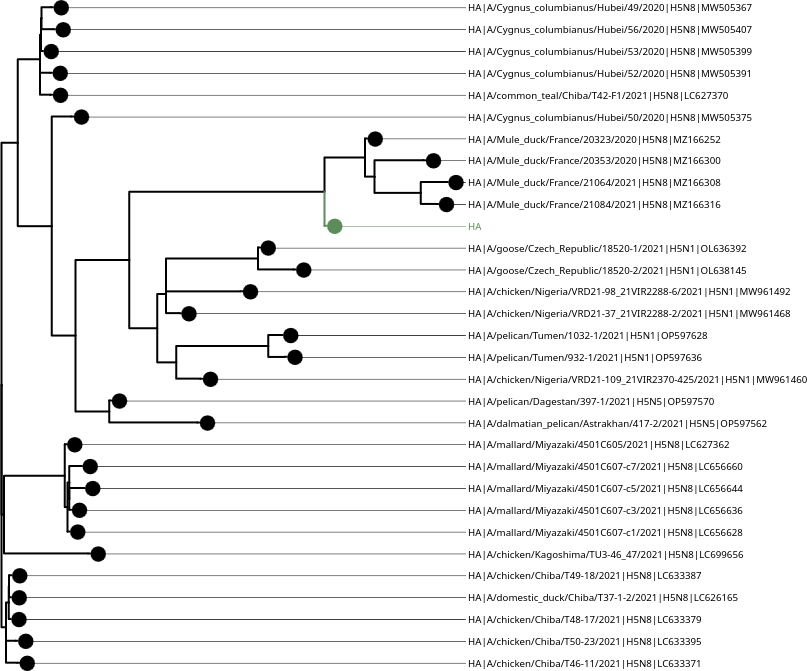
\includegraphics[width=1.0\textwidth]{media/4-aiv-s8-tree-ha.png}
        \caption{Phylogenetic tree of HA gene of H5N8 sample.}
		\label{fig:apx-aiv-trees-s8-ha}
    \end{subfigure} \\ 
	\vspace*{20pt}
    \begin{subfigure}[]{0.5\textheight}
        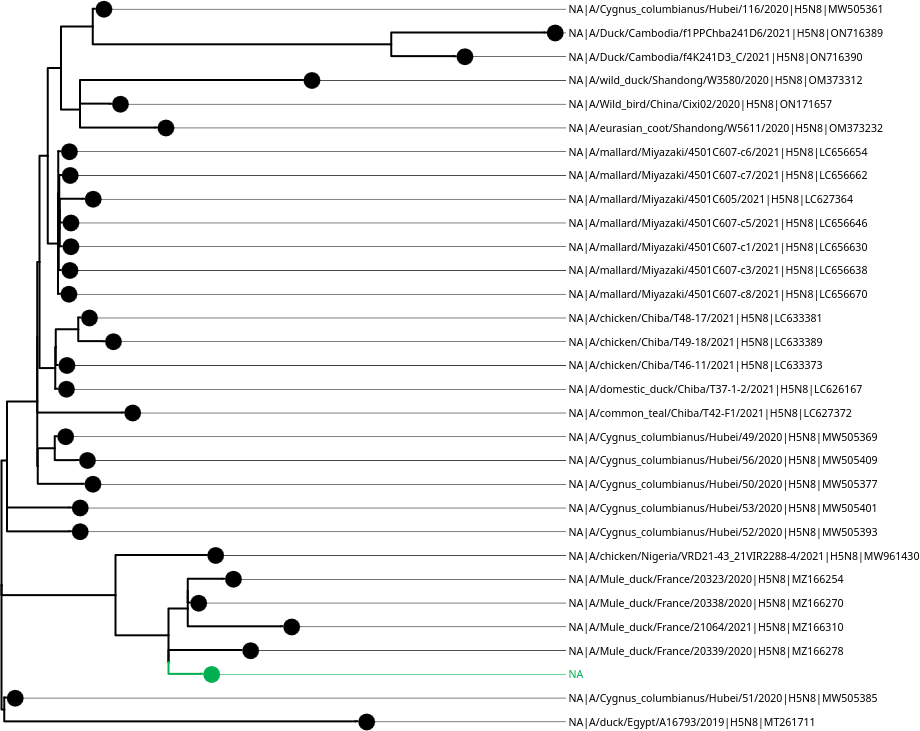
\includegraphics[width=1.0\textwidth]{media/4-aiv-s8-tree-na.png}
        \caption{Phylogenetic tree of NA gene of H5N8 sample.}
		\label{fig:apx-aiv-trees-s8-na}
    \end{subfigure} 
	\caption[Phylogenetic trees of HA and NA genes for H5N8 sample.]{Phylogenetic trees of HA and NA genes for H5N8 sample, indicating linkage to \textit{A/Mule\_duck/France} in both the HA and NA segments.}
\label{fig:apx-aiv-trees-s8}
\end{figure}


\hspace*{-36pt}
\renewcommand{\arraystretch}{1.3}
\begin{table}[ht!]
	\centering
	\begin{tabular}{ccccccccc}
		\multicolumn{9}{l}{Assembly}                                                                                                                                                                                                                                                                                                                                                                                                                                                                                                                                                                                    \\ \hline
		\multicolumn{1}{c|}{\textbf{Run \#}} & \multicolumn{4}{l|}{\textbf{Wall clock time}}                                                                                                                                                                                                                                               & \multicolumn{4}{l}{\textbf{Max. memory usage}}                                                                                                                                                                                                                             \\ \cline{2-9} 
		\multicolumn{1}{c|}{}                & \textbf{\begin{tabular}[c]{@{}c@{}}A\\ {[}s{]}\end{tabular}} & \textbf{\begin{tabular}[c]{@{}c@{}}Asia-1\\ {[}s{]}\end{tabular}} & \textbf{\begin{tabular}[c]{@{}c@{}}SAT-1\\ {[}s{]}\end{tabular}} & \multicolumn{1}{c|}{\textbf{\begin{tabular}[c]{@{}c@{}}SAT-2\\ {[}s{]}\end{tabular}}} & \textbf{\begin{tabular}[c]{@{}c@{}}A\\ {[}GB{]}\end{tabular}} & \textbf{\begin{tabular}[c]{@{}c@{}}Asia-1\\ {[}MB{]}\end{tabular}} & \textbf{\begin{tabular}[c]{@{}c@{}}SAT-1\\ {[}GB{]}\end{tabular}} & \textbf{\begin{tabular}[c]{@{}c@{}}SAT-2\\ {[}MB{]}\end{tabular}} \\ \hline
		\multicolumn{1}{c|}{1}               & 230                                                          & 272                                                               & 206                                                              & \multicolumn{1}{c|}{441}                                                              & 2.6                                                           & 2252.8                                                             & 1.1                                                               & 2150.4                                                            \\
		\multicolumn{1}{c|}{2}               & 156                                                          & 59                                                                & 298                                                              & \multicolumn{1}{c|}{28}                                                               & 2.6                                                           & 719.2                                                              & 1.1                                                               & 2150.4                                                            \\
		\multicolumn{1}{c|}{3}               & 92                                                           & 198                                                               & 88                                                               & \multicolumn{1}{c|}{26}                                                               & 2.8                                                           & 646.5                                                              & 2.3                                                               & 438.5                                                             \\
		\multicolumn{1}{c|}{4}               & 86                                                           & 335                                                               & 39                                                               & \multicolumn{1}{c|}{30}                                                               & 2.6                                                           & 2252.8                                                             & 2.3                                                               & 227.5                                                             \\
		\multicolumn{1}{c|}{5}               & 115                                                          & 142                                                               & 707                                                              & \multicolumn{1}{c|}{20}                                                               & 2.4                                                           & 648.8                                                              & 2.3                                                               & 1740.8                                                            \\
		\multicolumn{1}{c|}{6}               & 104                                                          & 134                                                               & 271                                                              & \multicolumn{1}{c|}{174}                                                              & 2.4                                                           & 648.2                                                              & 1.1                                                               & 2150.4                                                            \\
		\multicolumn{1}{c|}{7}               & 117                                                          & 54                                                                & 241                                                              & \multicolumn{1}{c|}{174}                                                              & 2.6                                                           & 665.6                                                              & 2.3                                                               & 2150.4                                                            \\
		\multicolumn{1}{c|}{8}               & 439                                                          & 31                                                                & 59                                                               & \multicolumn{1}{c|}{20}                                                               & 2.7                                                           & 641.7                                                              & 1.4                                                               & 497.6                                                             \\
		\multicolumn{1}{c|}{9}               & 310                                                          & 215                                                               & 52                                                               & \multicolumn{1}{c|}{38}                                                               & 2.7                                                           & 2252.8                                                             & 2.1                                                               & 2150.4                                                            \\
		\multicolumn{1}{c|}{10}              & 440                                                          & 126                                                               & 386                                                              & \multicolumn{1}{c|}{32}                                                               & 2.7                                                           & 653.9                                                              & 1.1                                                               & 209.6                                                             \\ \hline
		\textbf{Average}                     & \textbf{208.9}                                               & \textbf{156.6}                                                    & \textbf{234.7}                                                   & \textbf{98.3}                                                                         & \textbf{2.61}                                                 & \textbf{1138.23}                                                   & \textbf{1.71}                                                     & \textbf{1386.6}                                                   \\ \hline
		\multicolumn{9}{l}{\begin{tabular}[c]{@{}c@{}}{ }\\Mapping\end{tabular}}                                                                                                                                                                                                                                                                                                                                                                                                                                                                                                                                                                                     \\ \hline
		\multicolumn{1}{c|}{\textbf{Run \#}} & \multicolumn{4}{l|}{\textbf{Wall clock time}}                                                                                                                                                                                                                                               & \multicolumn{4}{l}{\textbf{Max. memory usage}}                                                                                                                                                                                                                             \\ \cline{2-9} 
		\multicolumn{1}{l|}{}                & \textbf{\begin{tabular}[c]{@{}c@{}}A\\ {[}s{]}\end{tabular}} & \textbf{\begin{tabular}[c]{@{}c@{}}Asia-1\\ {[}s{]}\end{tabular}} & \textbf{\begin{tabular}[c]{@{}c@{}}SAT-1\\ {[}s{]}\end{tabular}} & \multicolumn{1}{c|}{\textbf{\begin{tabular}[c]{@{}c@{}}SAT-2\\ {[}s{]}\end{tabular}}} & \textbf{\begin{tabular}[c]{@{}c@{}}A\\ {[}GB{]}\end{tabular}} & \textbf{\begin{tabular}[c]{@{}c@{}}Asia-1\\ {[}MB{]}\end{tabular}} & \textbf{\begin{tabular}[c]{@{}c@{}}SAT-1\\ {[}MB{]}\end{tabular}} & \textbf{\begin{tabular}[c]{@{}c@{}}SAT-2\\ {[}MB{]}\end{tabular}} \\ \hline
		\multicolumn{1}{c|}{1}               & 51                                                           & 23                                                                & 50                                                               & \multicolumn{1}{c|}{31}                                                               & 1.4                                                           & 577.6                                                              & 823.5                                                             & 182.1                                                             \\
		\multicolumn{1}{c|}{2}               & 40                                                           & 27                                                                & 30                                                               & \multicolumn{1}{c|}{16}                                                               & 1.4                                                           & 576.2                                                              & 816.9                                                             & 184.2                                                             \\
		\multicolumn{1}{c|}{3}               & 50                                                           & 18                                                                & 39                                                               & \multicolumn{1}{c|}{15}                                                               & 1.4                                                           & 576.1                                                              & 824.7                                                             & 182.9                                                             \\
		\multicolumn{1}{c|}{4}               & 95                                                           & 24                                                                & 43                                                               & \multicolumn{1}{c|}{15}                                                               & 1.4                                                           & 576.2                                                              & 823.8                                                             & 182.5                                                             \\
		\multicolumn{1}{c|}{5}               & 69                                                           & 19                                                                & 31                                                               & \multicolumn{1}{c|}{37}                                                               & 1.4                                                           & 576.5                                                              & 826.0                                                             & 182.0                                                             \\
		\multicolumn{1}{c|}{6}               & 70                                                           & 21                                                                & 26                                                               & \multicolumn{1}{c|}{34}                                                               & 1.4                                                           & 573.6                                                              & 819.3                                                             & 181.7                                                             \\
		\multicolumn{1}{c|}{7}               & 60                                                           & 23                                                                & 33                                                               & \multicolumn{1}{c|}{20}                                                               & 1.4                                                           & 580.4                                                              & 821.5                                                             & 181.5                                                             \\
		\multicolumn{1}{c|}{8}               & 57                                                           & 23                                                                & 23                                                               & \multicolumn{1}{c|}{13}                                                               & 1.4                                                           & 574.1                                                              & 823.0                                                             & 183.1                                                             \\
		\multicolumn{1}{c|}{9}               & 65                                                           & 17                                                                & 47                                                               & \multicolumn{1}{c|}{20}                                                               & 1.4                                                           & 576.8                                                              & 823.6                                                             & 185.8                                                             \\
		\multicolumn{1}{c|}{10}              & 59                                                           & 20                                                                & 77                                                               & \multicolumn{1}{c|}{39}                                                               & 1.4                                                           & 576.8                                                              & 824.9                                                             & 181.7                                                             \\ \hline
		\textbf{Average}                     & \textbf{61.6}                                                & \textbf{21.5}                                                     & \textbf{39.9}                                                    & \textbf{24.0}                                                                         & \textbf{1.4}                                                  & \textbf{576.43}                                                    & \textbf{822.72}                                                   & \textbf{182.75}                                                   \\ \hline
	\end{tabular}
	\caption[Raw profiling data to compare assembly and reference-based mapping with FMDV samples.]{Raw profiling data for assembly with \texttt{rnaviralSPAdes} (top) and mapping with \texttt{BWA-MEM} (bottom) on four FMDV samples on Galaxy.}
\label{tab:fmdv-profiling}
\end{table}
% smallest EC2 machine we could find is m5d.4xlarge (64 GB / 16 vCPUs / Intel Xeon Platinum 8175). 
% smallest EC2 machine we could find is m3.2xlarge (30 GB / 8 vCPUs / Intel Xeon E5-2670 v2 (Ivy Bridge/Sandy Bridge))
    \addcontentsline{toc}{chapter}{Appendix}
    \newpage
    \thispagestyle{empty}
    \mbox{}

\end{document}
